Queremos observar que tan bueno es el algoritmo propuesto en la práctica. Para esto realizaremos una serie de tests utilizando las entradas que se utilizaron en el ejercicio 3.
La idea es tratar de encontrar la configuración ideal para que en promedio el algoritmo resuelva la mayoria de los casos eficientemente. Para lograr esto, experimentamos variando distintos parametros para cada entrada y obtener las respectivas conclusiones de los resultados obtenidos.\\
Los parámetros de estudio fueron:

\begin{enumerate}
\item  \textbf{Cantidad de iteraciones}: Tenemos que observar en promedio, cuantas iteraciones conviene tomar para obtener un buen resutado.
\item \textbf{Tenor tabú}: Tenemos que observar que sucede al aumentar el tenor tabú, y hasta cuanto es conveniente hacerlo para obtener un buen resultado.
\item \textbf{Atributos tabú}: Analizar que sucede al tomar como atributos tabú las aristas que cambiaron o las aristas nuevas
\item \textbf{Función de aspiración}: Elegir la solución más tabú o la menos tabú.
\end{enumerate}

Debemos aclarar, que tenor tabú fué establecido en cantidad de pokeparadas mas gimnasios. Este valor puede ser relativamente grande, pero cuanto más grande, más tiempo de resolución es necesario, con lo cual al final no es una cuestion de memoria, si no, una cuestion de tiempo de computos necesaria para correr el algoritmo.
También se trabajó probando diferentes configuraciones de atributos tabú y función de aspiración, obteniendo en todos los casos los mismos resultados, por lo que al final se decidió dejar prefijado el estandar para tabú search que es aristas viejas como atributos tabú y solución menos tabú para la función de aspiración.\\

Se tomaron 20 mediciones por cada tipo de test y se tomó una media alfa podada de las mismas con $\alpha$ = 0.5 de manera de podar un 25\% de los datos a cada lado.  De esta forma se reduce la posibilidad de outliers en las muestras consideradas.

Como fue enunciado en incisos anteriores de este trabajo las 4 familias en las que la heur\'istica golosa no otorga una soluci\'on \'optima son:

\begin{enumerate}
\item Familia 4
\item Familia 6
\item Familia 7
\item Familia 8
\end{enumerate}

Estas ser\'an las únicas a ser a analizadas, ya que el resto son el resultado exacto o no tienen soluci\'on, con lo cual no aportan mayor relevancia.
 
\subsubsection*{Familia 4}

Veamos algunos resultados de aplicar cada version de tabú search:

\vspace*{0.3cm} \vspace*{0.3cm}
  \begin{center}
 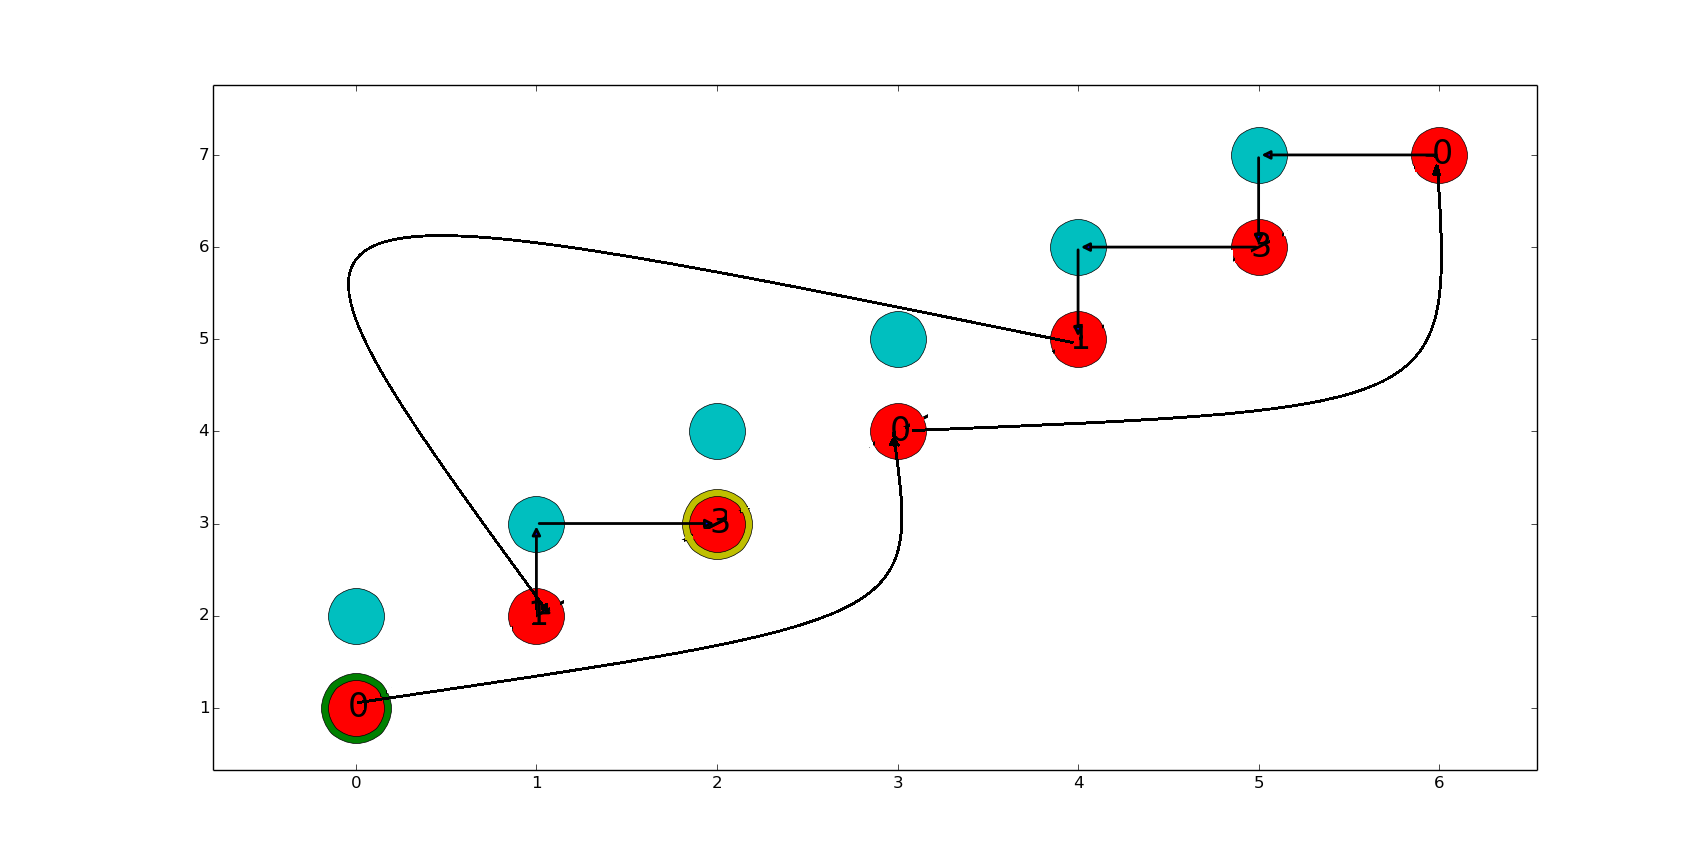
\includegraphics[scale=0.3]{./EJ4/fam4goloso.png}\\
 {            \textit{Soluci\'on Golosa}}
  \end{center}
  \vspace*{0.3cm}

\vspace*{0.3cm} \vspace*{0.3cm}
  \begin{center}
 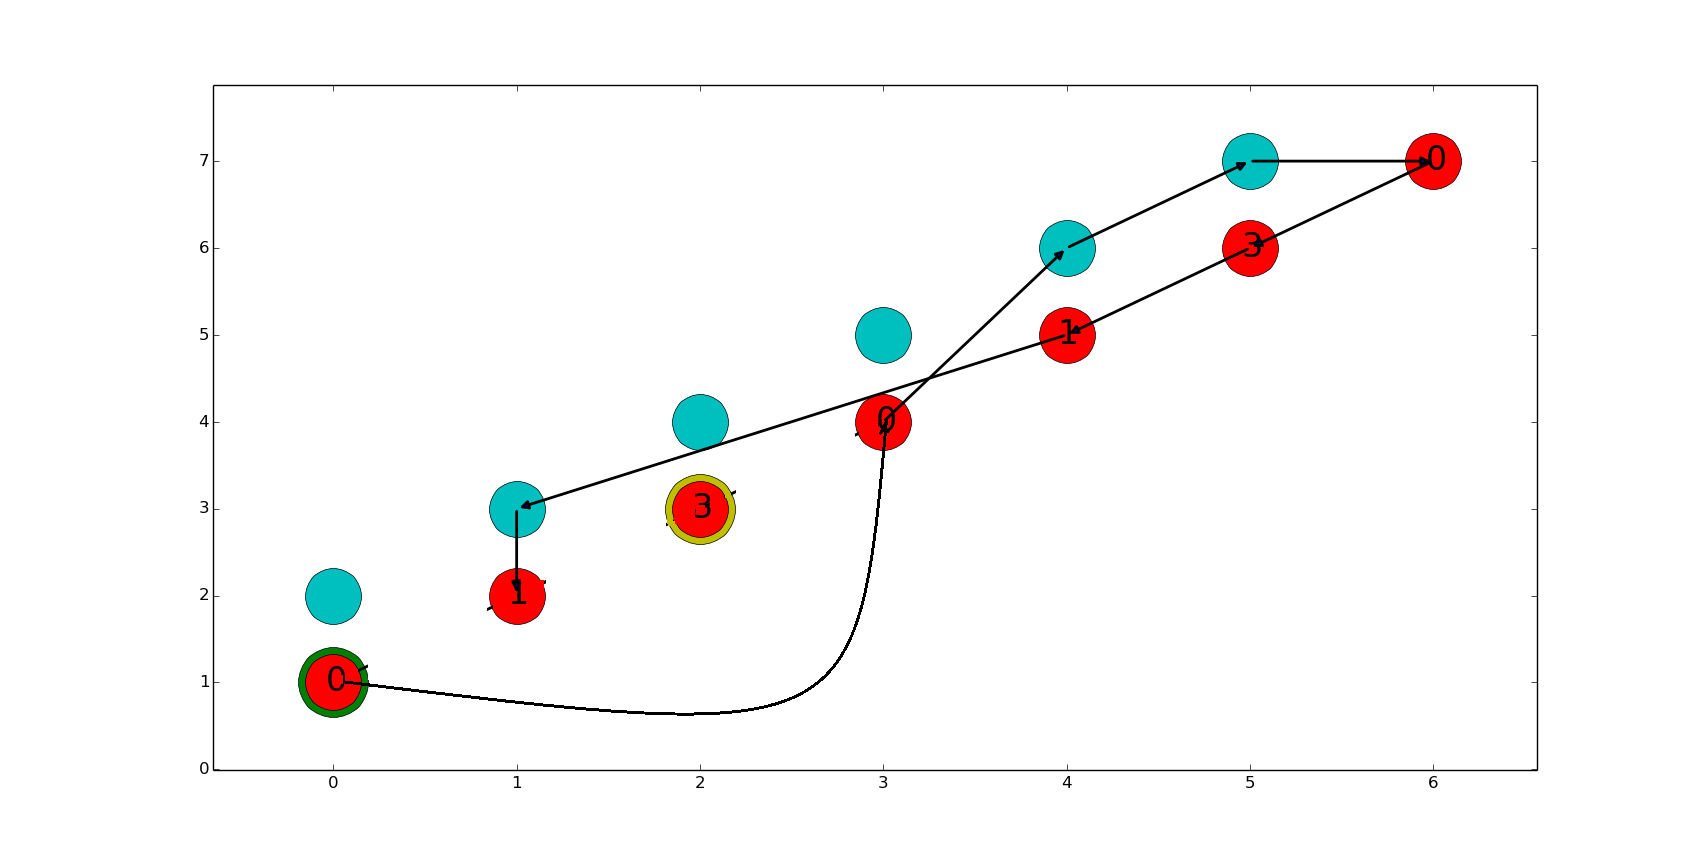
\includegraphics[scale=0.3]{./EJ4/fam42opt.png}\\
 {            \textit{Soluci\'on 2-OPT}}
  \end{center}
  \vspace*{0.3cm}

\vspace*{0.3cm} \vspace*{0.3cm}
  \begin{center}
 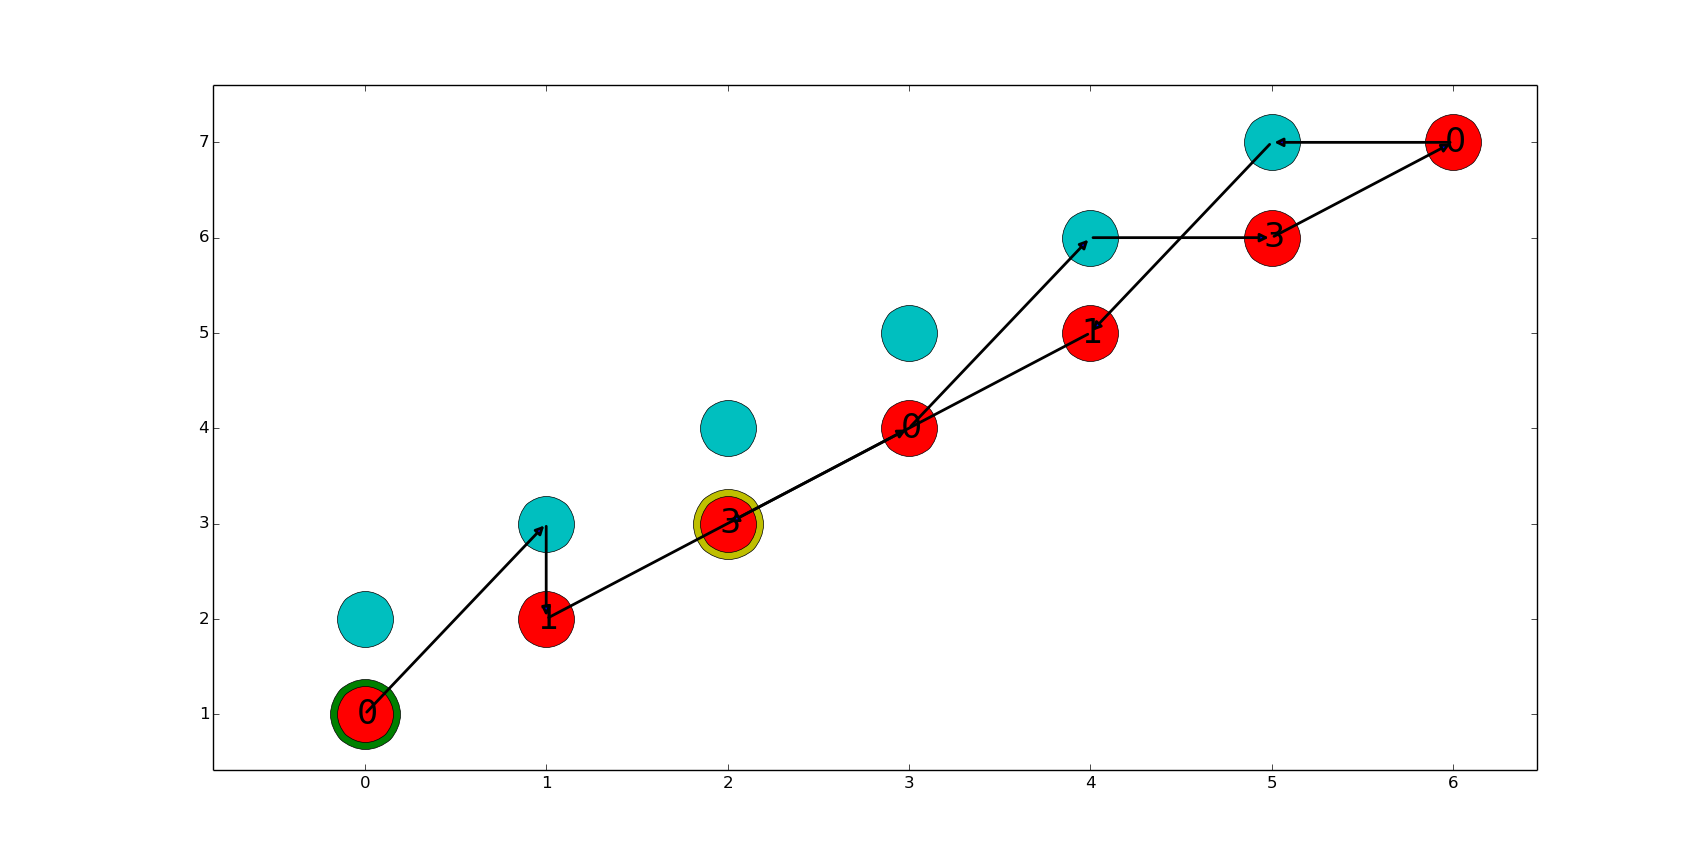
\includegraphics[scale=0.3]{./EJ4/fam43opt.png}\\
 {            \textit{Soluci\'on 3-OPT}}
  \end{center}
  \vspace*{0.3cm}

Nos parece interente comparar los resultados de mejora y tiempo de las búsquedas locales y tabú search que utilicen la misma vecindad, para ver si tabú search mejora lo logrado por la búsqueda local o empeora el resultado. Esto será realizado para cada familia mencionada.\\

Veamos como se comporta tabú 2-OPT con respecto a la heuristica de búsqueda local 2-OPT dentro de la familia 4:

\vspace*{0.3cm} \vspace*{0.3cm}
  \begin{center}
 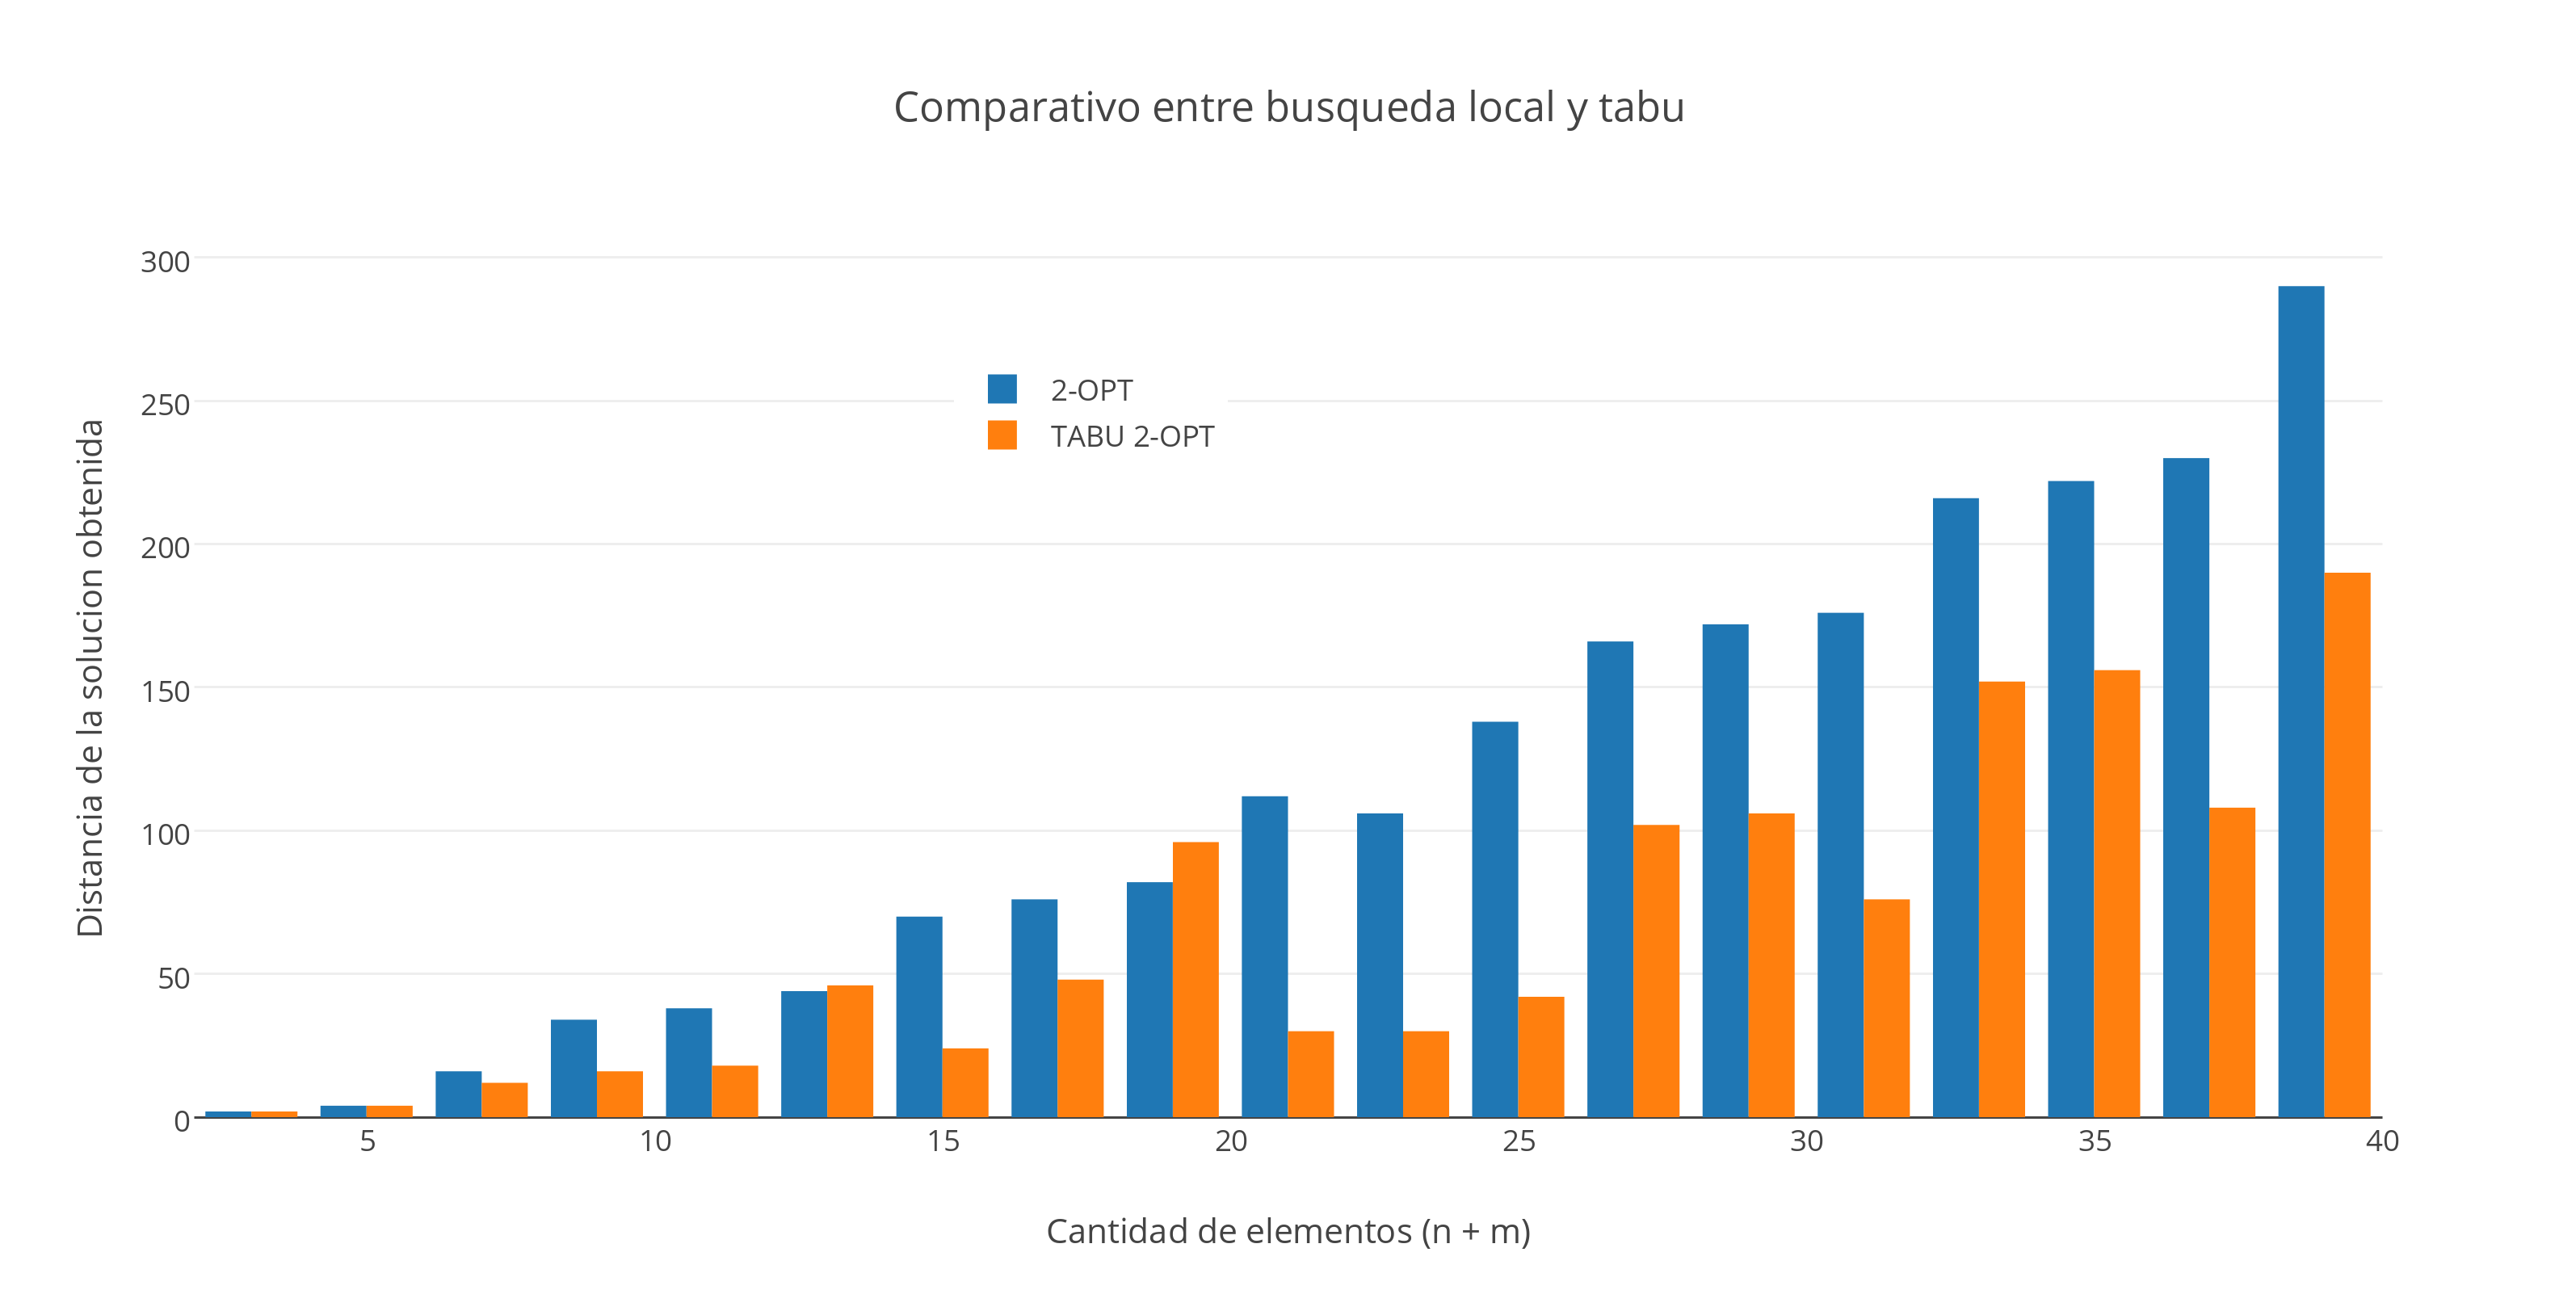
\includegraphics[scale=0.5]{./EJ4/comparativogym02opt.png}\\
 {            \textit{Gráfico \ 4.1 - 2-OPT vs Tabu 2-OPT sobre Familia 4}}
  \end{center}
  \vspace*{0.3cm}

En cuanto a tiempo insumido vemos lo siguiente:

\vspace*{0.3cm} \vspace*{0.3cm}
  \begin{center}
 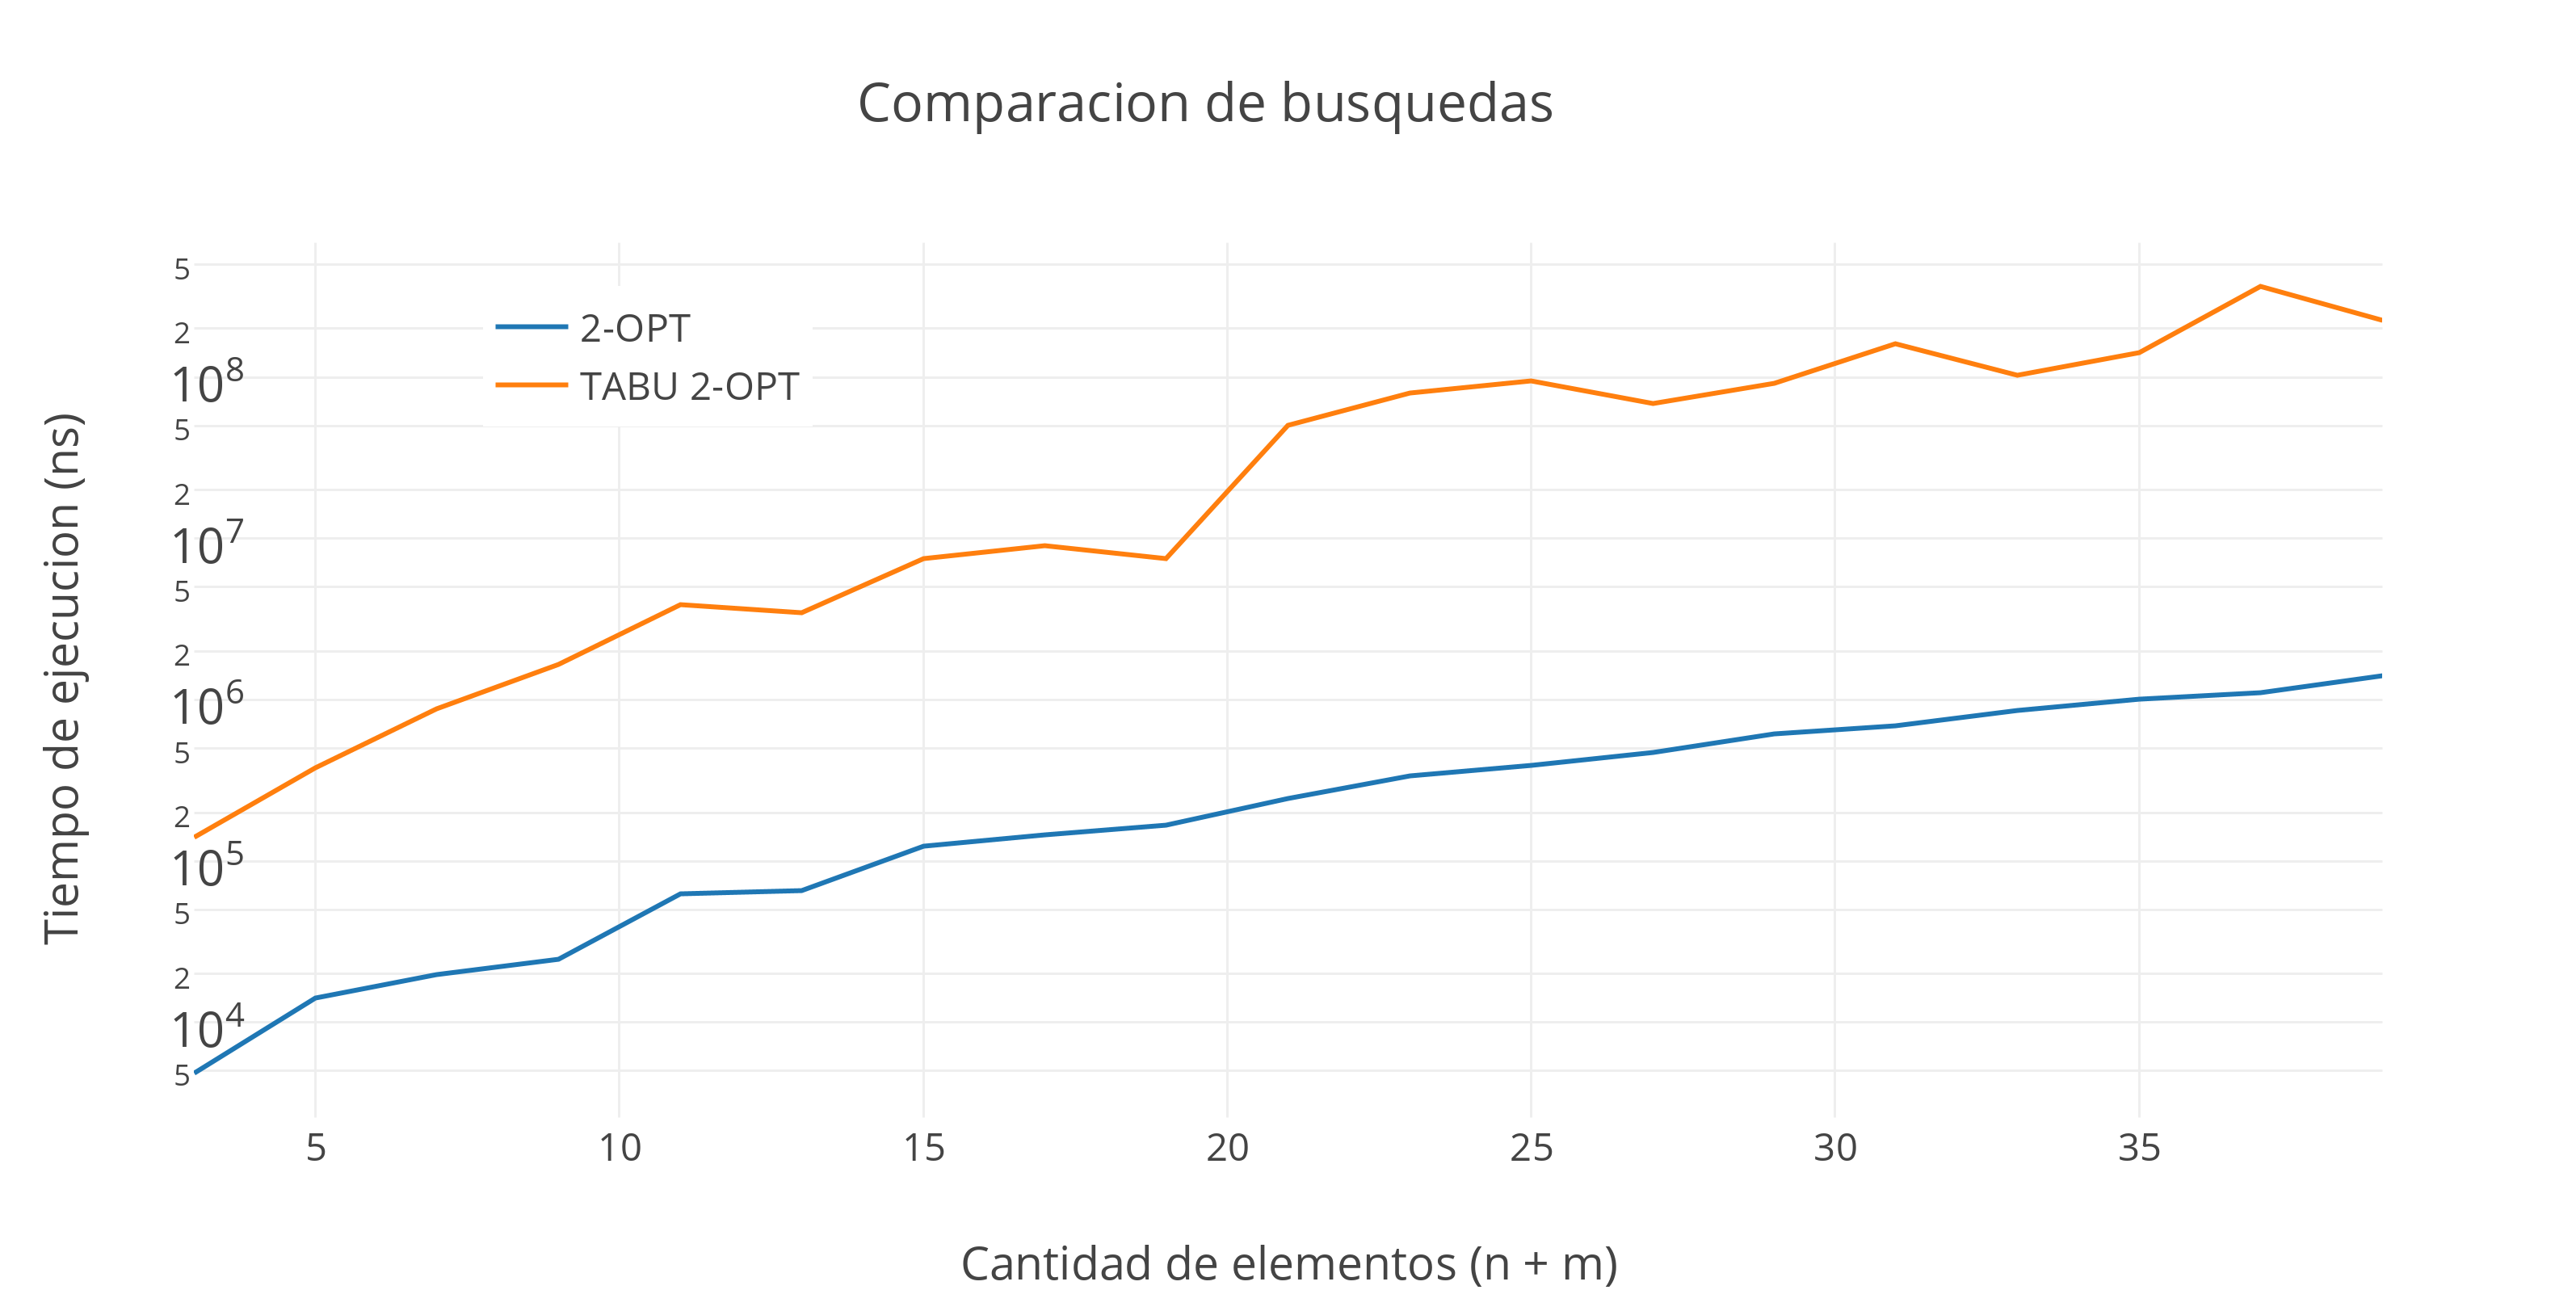
\includegraphics[scale=0.5]{./EJ4/medicion2optgym0.png}\\
 {            \textit{Gráfico \ 4.2 - 2-OPT vs Tabu 2-OPT sobre Familia 4}}
  \end{center}
  \vspace*{0.3cm}
  
 Aplicando 3-OPT:

\vspace*{0.3cm} \vspace*{0.3cm}
  \begin{center}
 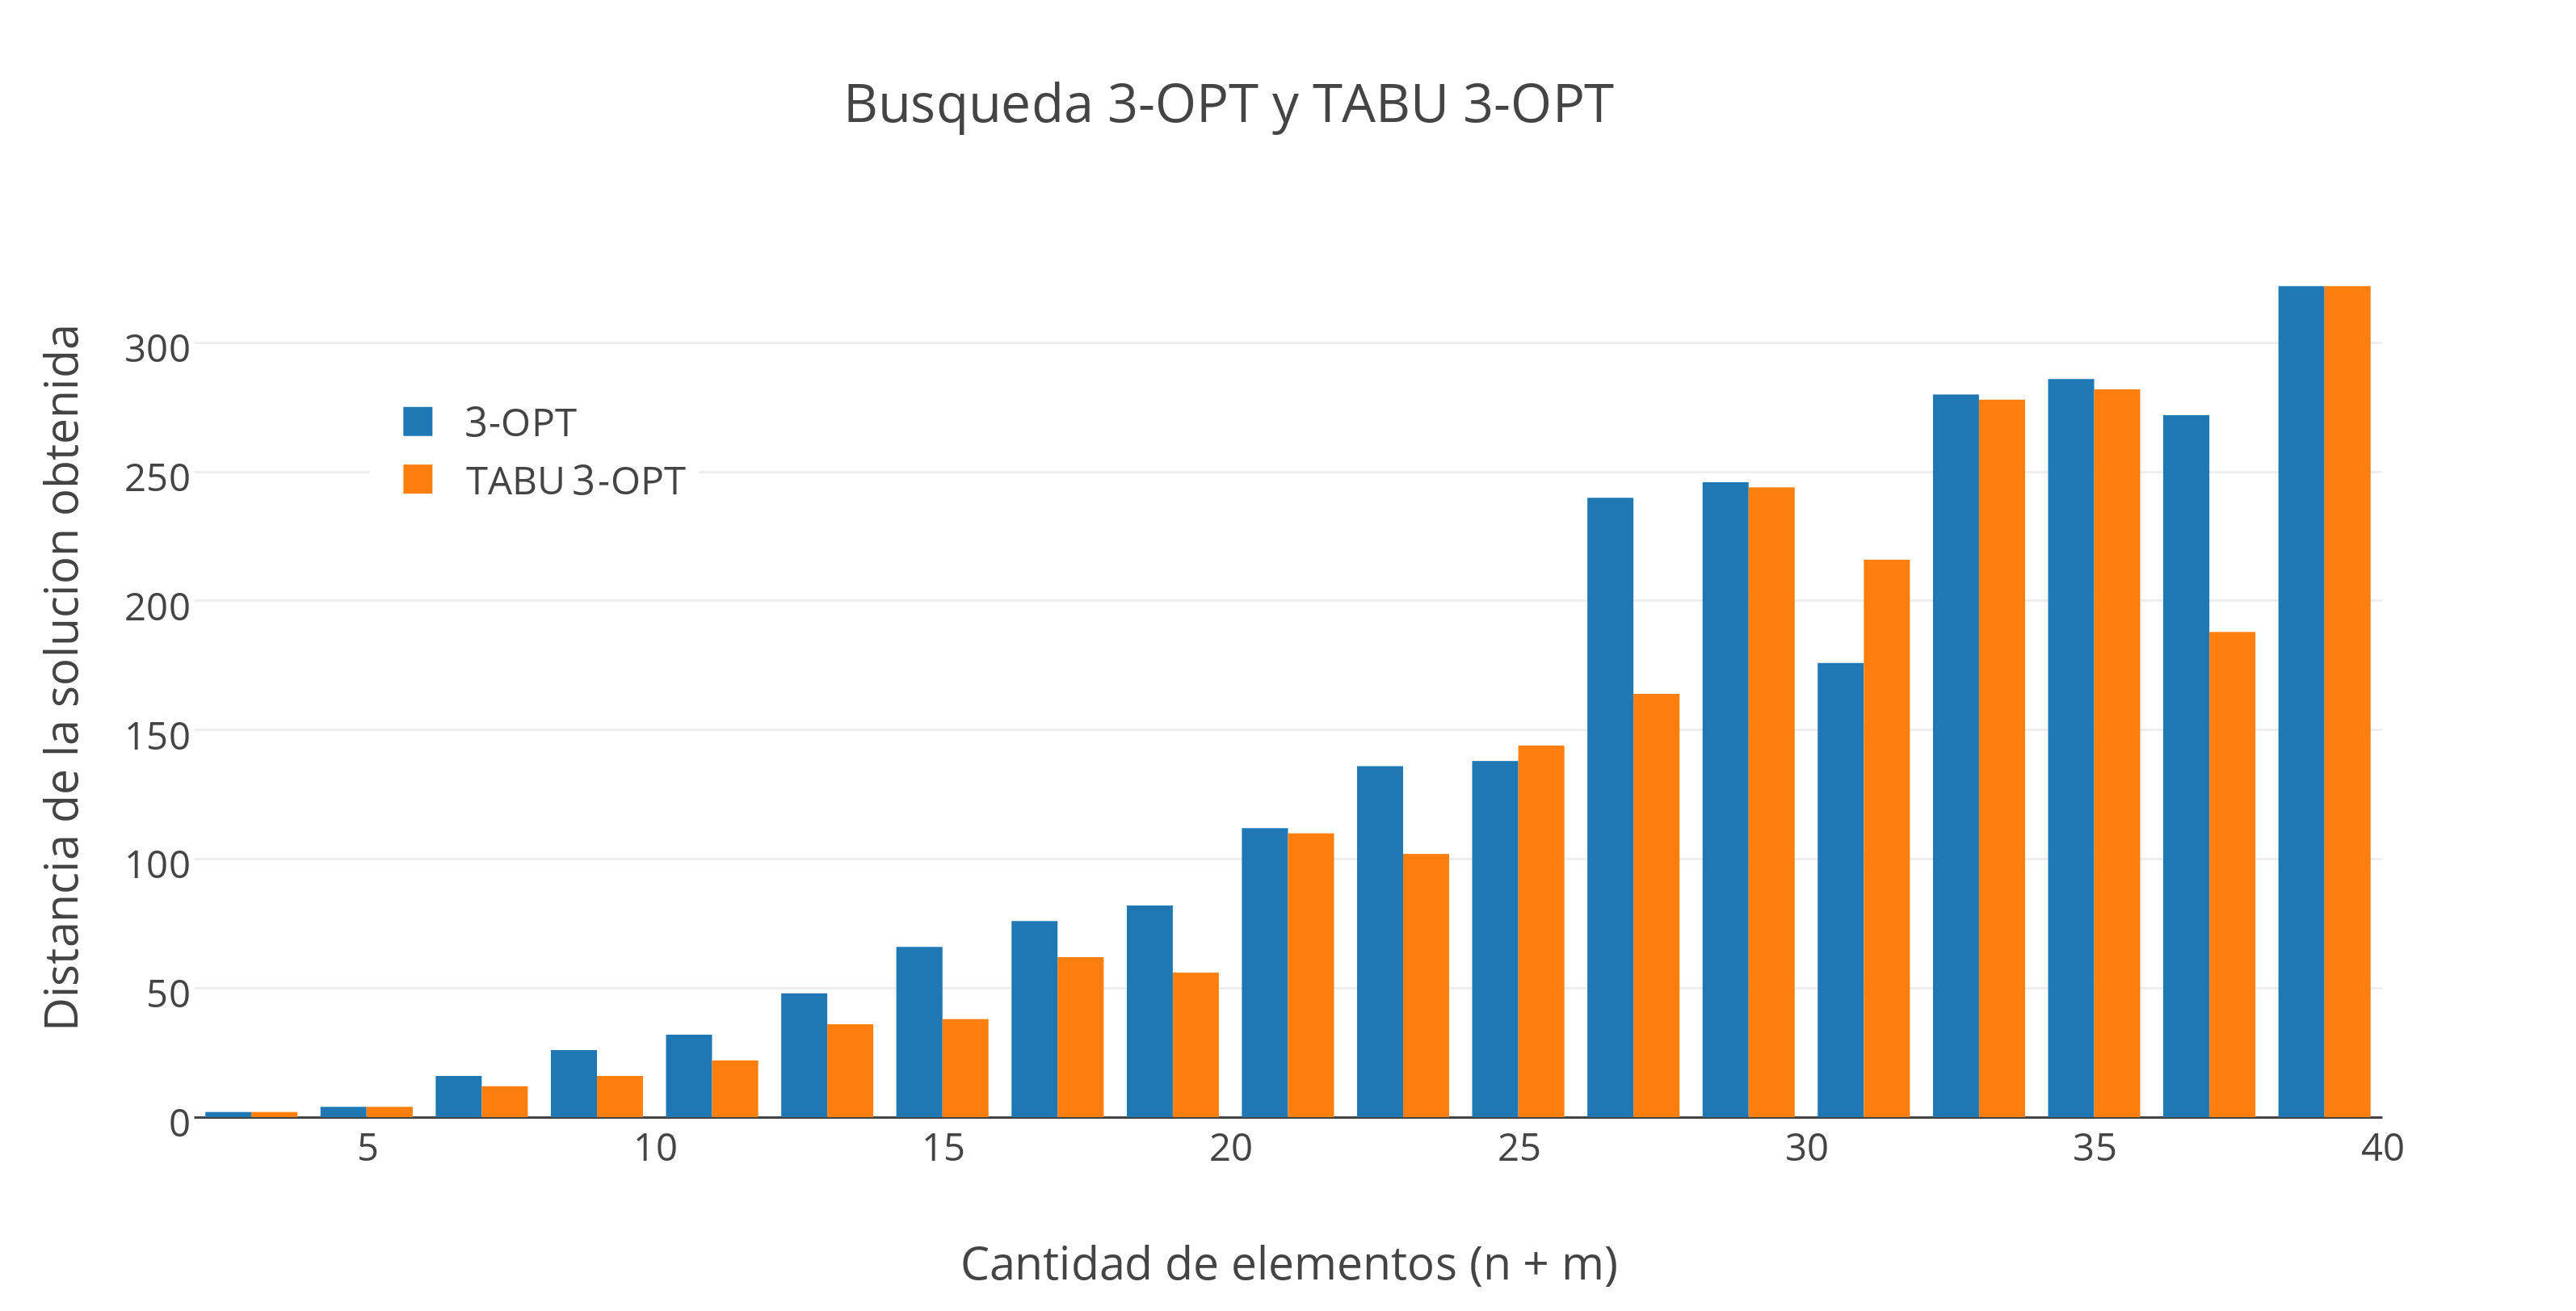
\includegraphics[scale=0.5]{./EJ4/comparativogym03opt.png}\\
 {            \textit{Gráfico \ 4.3 - 3-OPT vs Tabu 3-OPT sobre Familia 4}}
  \end{center}
  \vspace*{0.3cm}

\vspace*{0.3cm} \vspace*{0.3cm}
  \begin{center}
 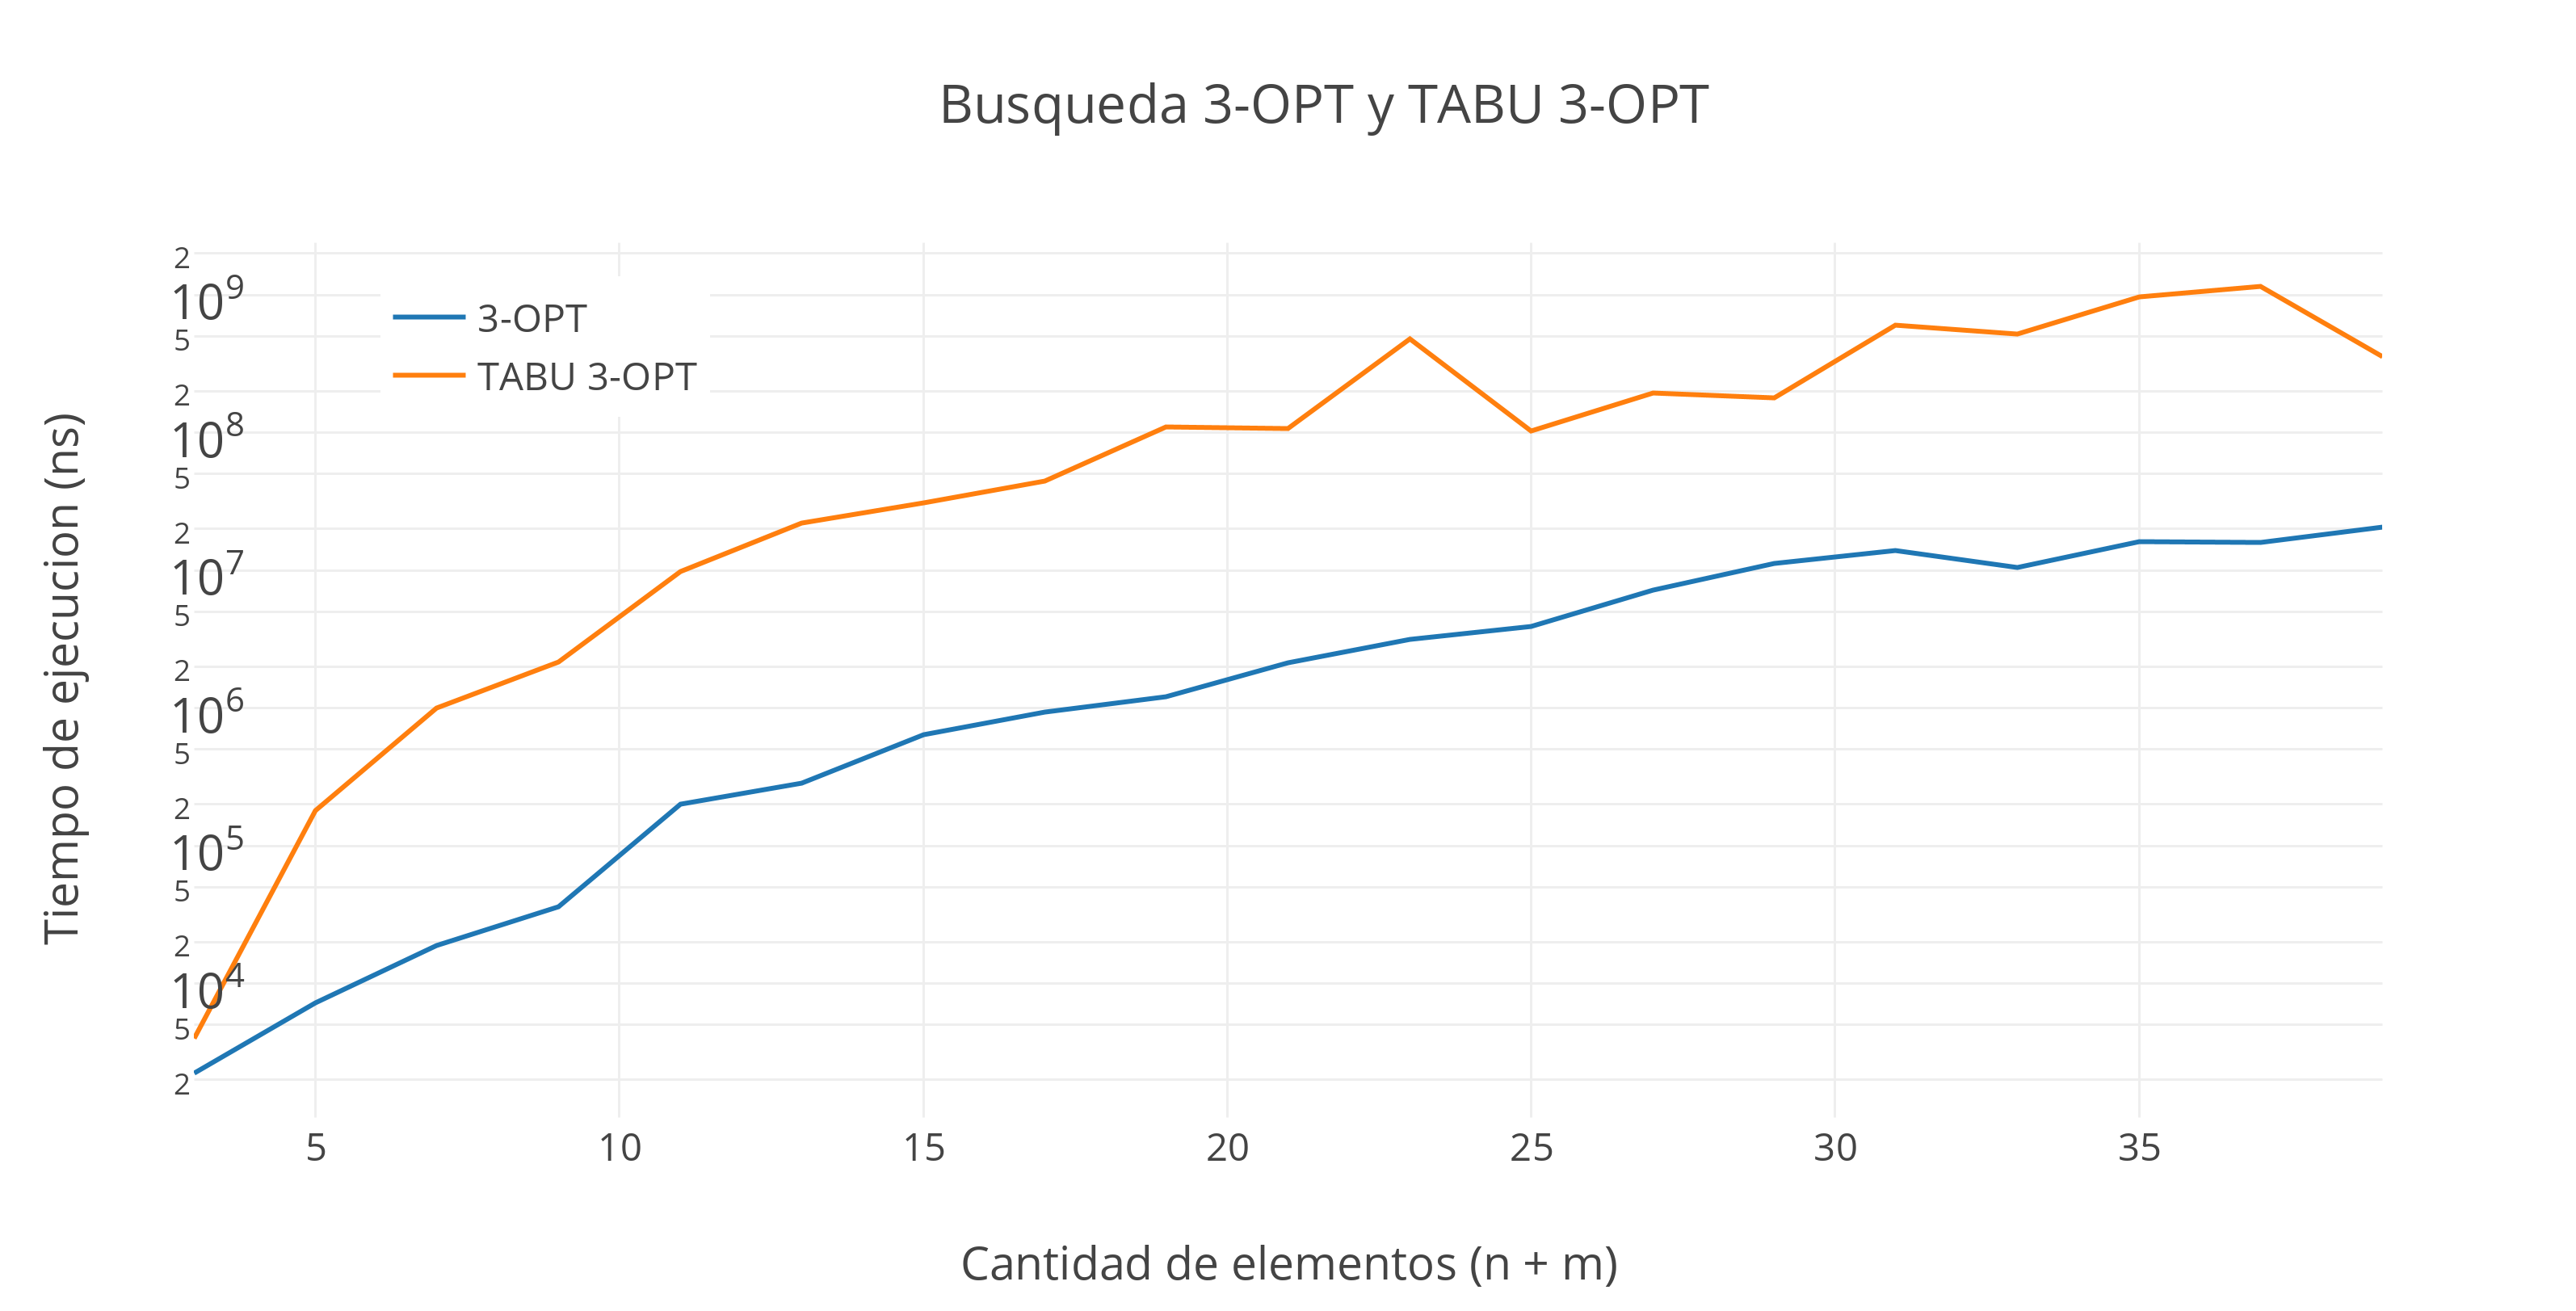
\includegraphics[scale=0.5]{./EJ4/medicion3optgym0.png}\\
 {            \textit{Gráfico \ 4.4 - 3-OPT vs Tabu 3-OPT sobre Familia 4}}
  \end{center}
  \vspace*{0.3cm}
  
Podemos observar que tabú search 2-OPT mejora lo realizado por la heuristica de búsqueda local 2-OPT. Los tiempos insumidos para lograrlo son elevados, pero en relación a la mejora es un resultado aceptable en la práctica. No así tabú search 3-OPT que apenas mejora lo realizado por búsqueda local 3-OPT y requiere tiempos elevados de corrida del algoritmo.\\
  
Para decidir que vecindad es mejor utilizar en tabú search, se comparará conjuntamente el tiempo de ejecución con la calidad de la solución. Para esta última tendremos en cuenta que los algoritmos, de devolver un resultado, serán válidos: esto quiere decir que cuanto menor distancia recorran las soluciones, mejor serán las mismas:

Las soluciones obtenidas fueron las siguientes:

\vspace*{0.3cm} \vspace*{0.3cm}
  \begin{center}
 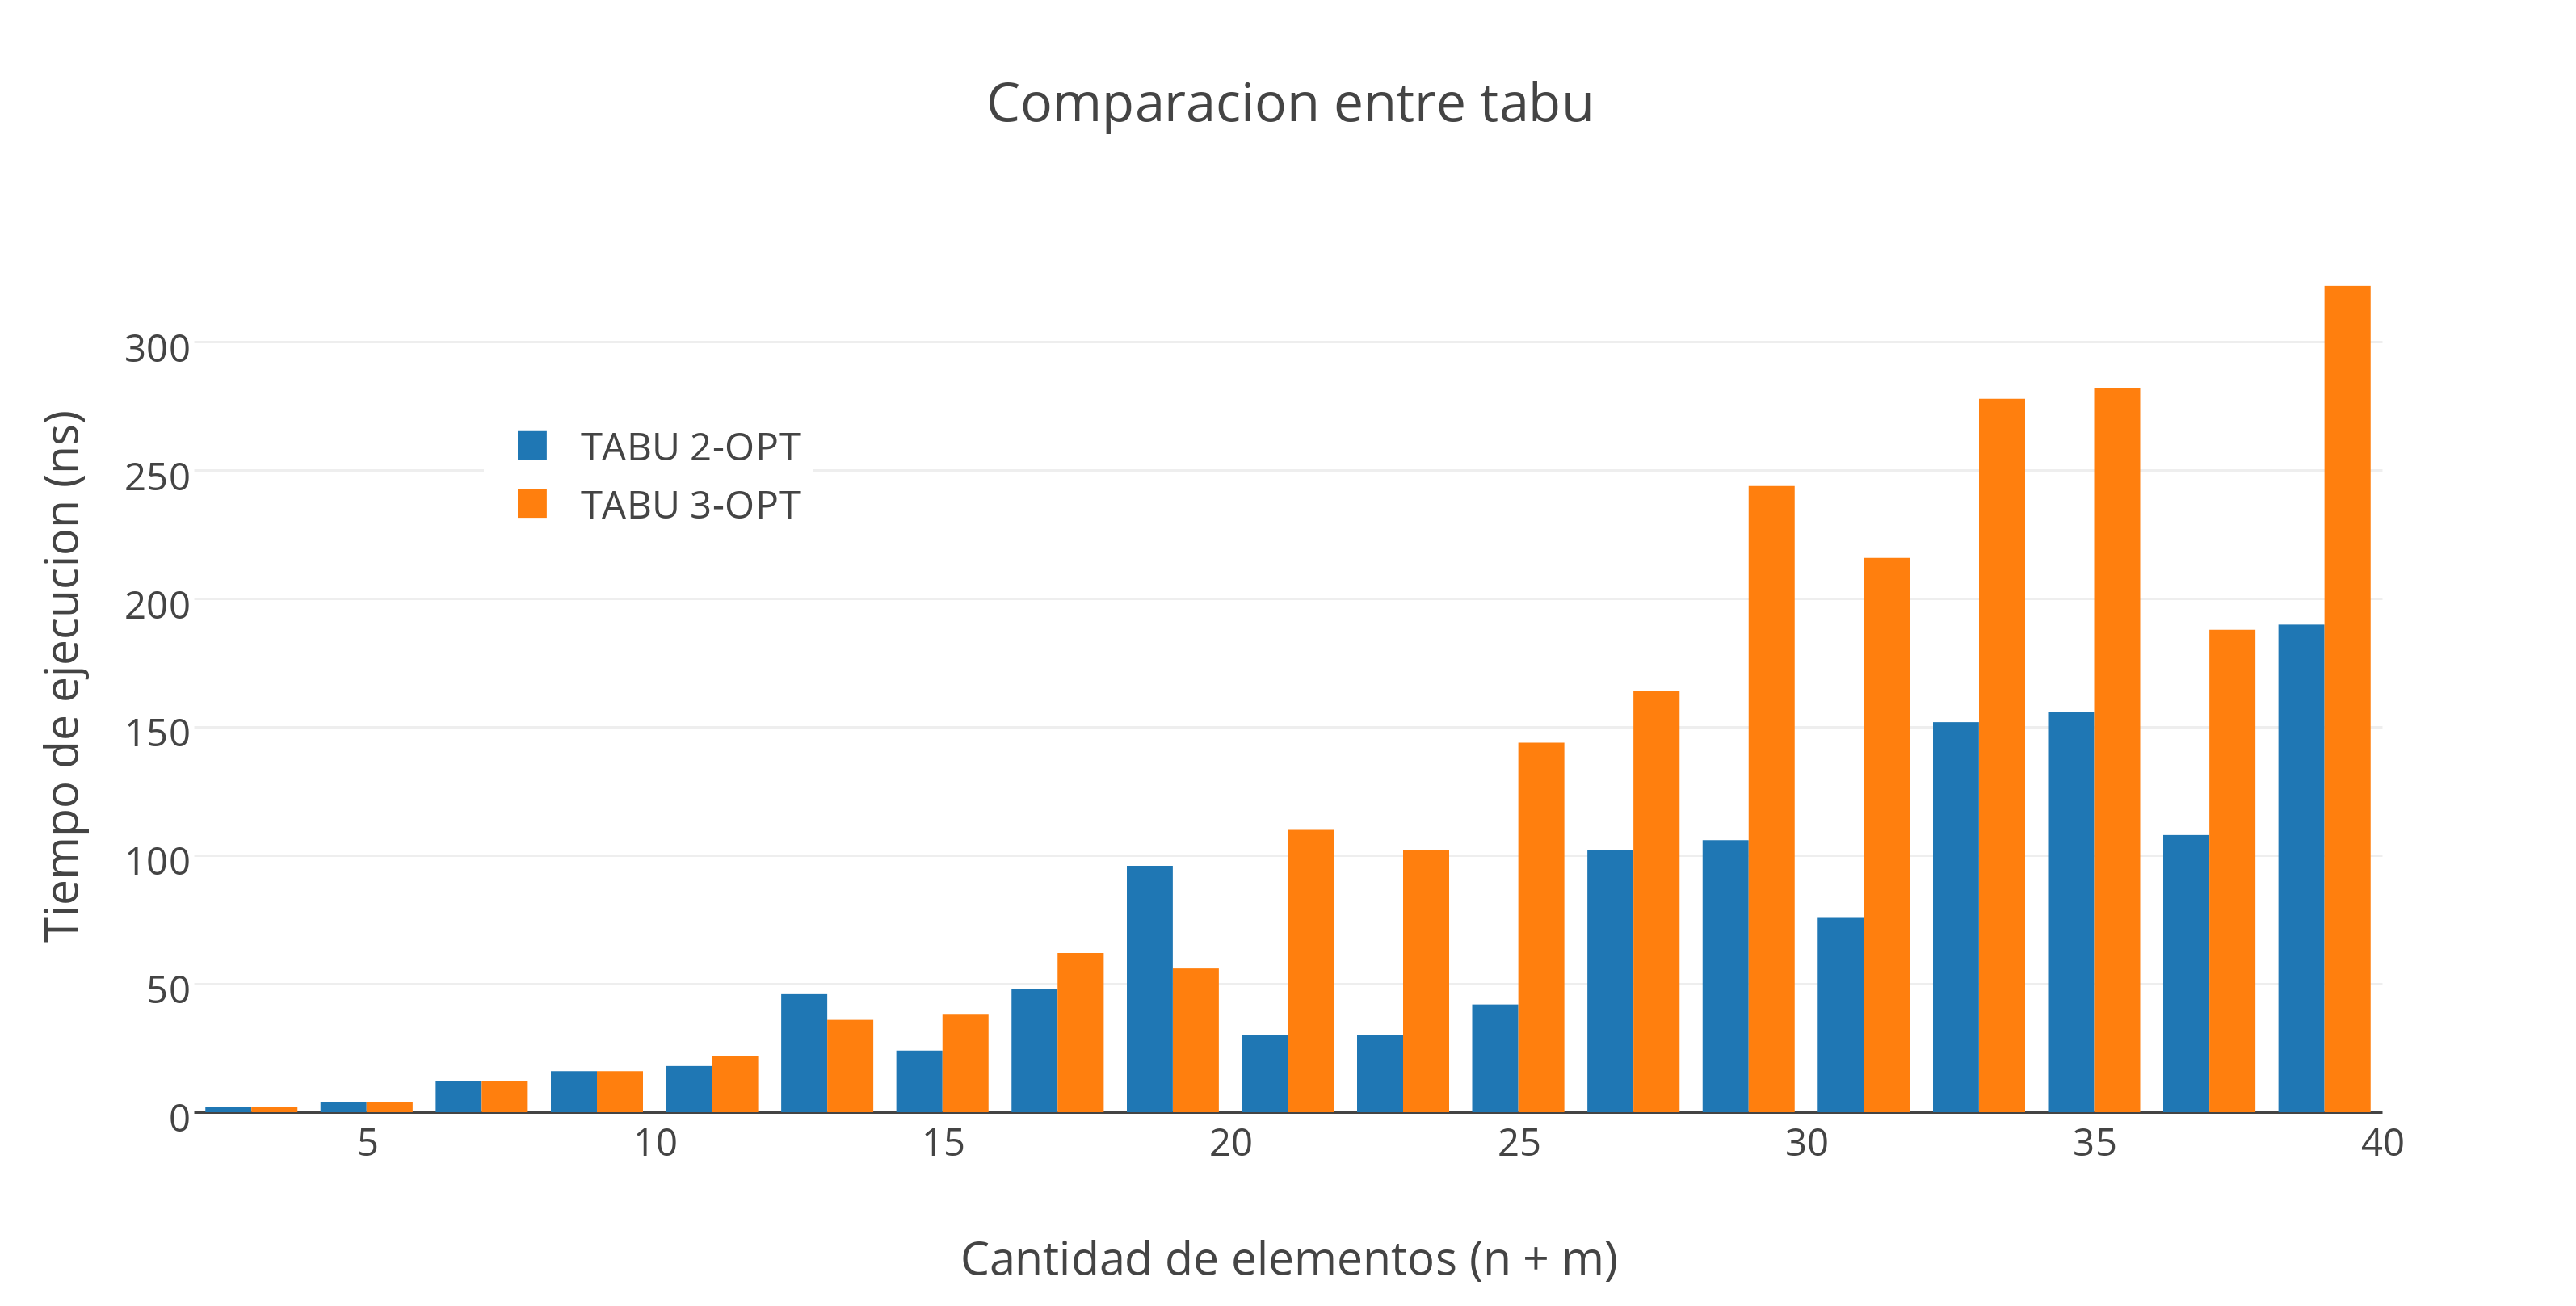
\includegraphics[scale=0.5]{./EJ4/comparativogym0.png}\\
 {            \textit{Gráfico \ 4.5 - Tabu 2-OPT vs Tabu 3-OPT sobre Familia 4}}
  \end{center}
  \vspace*{0.3cm}

En cuanto a tiempo insumido vemos lo siguiente:

\vspace*{0.3cm} \vspace*{0.3cm}
  \begin{center}
 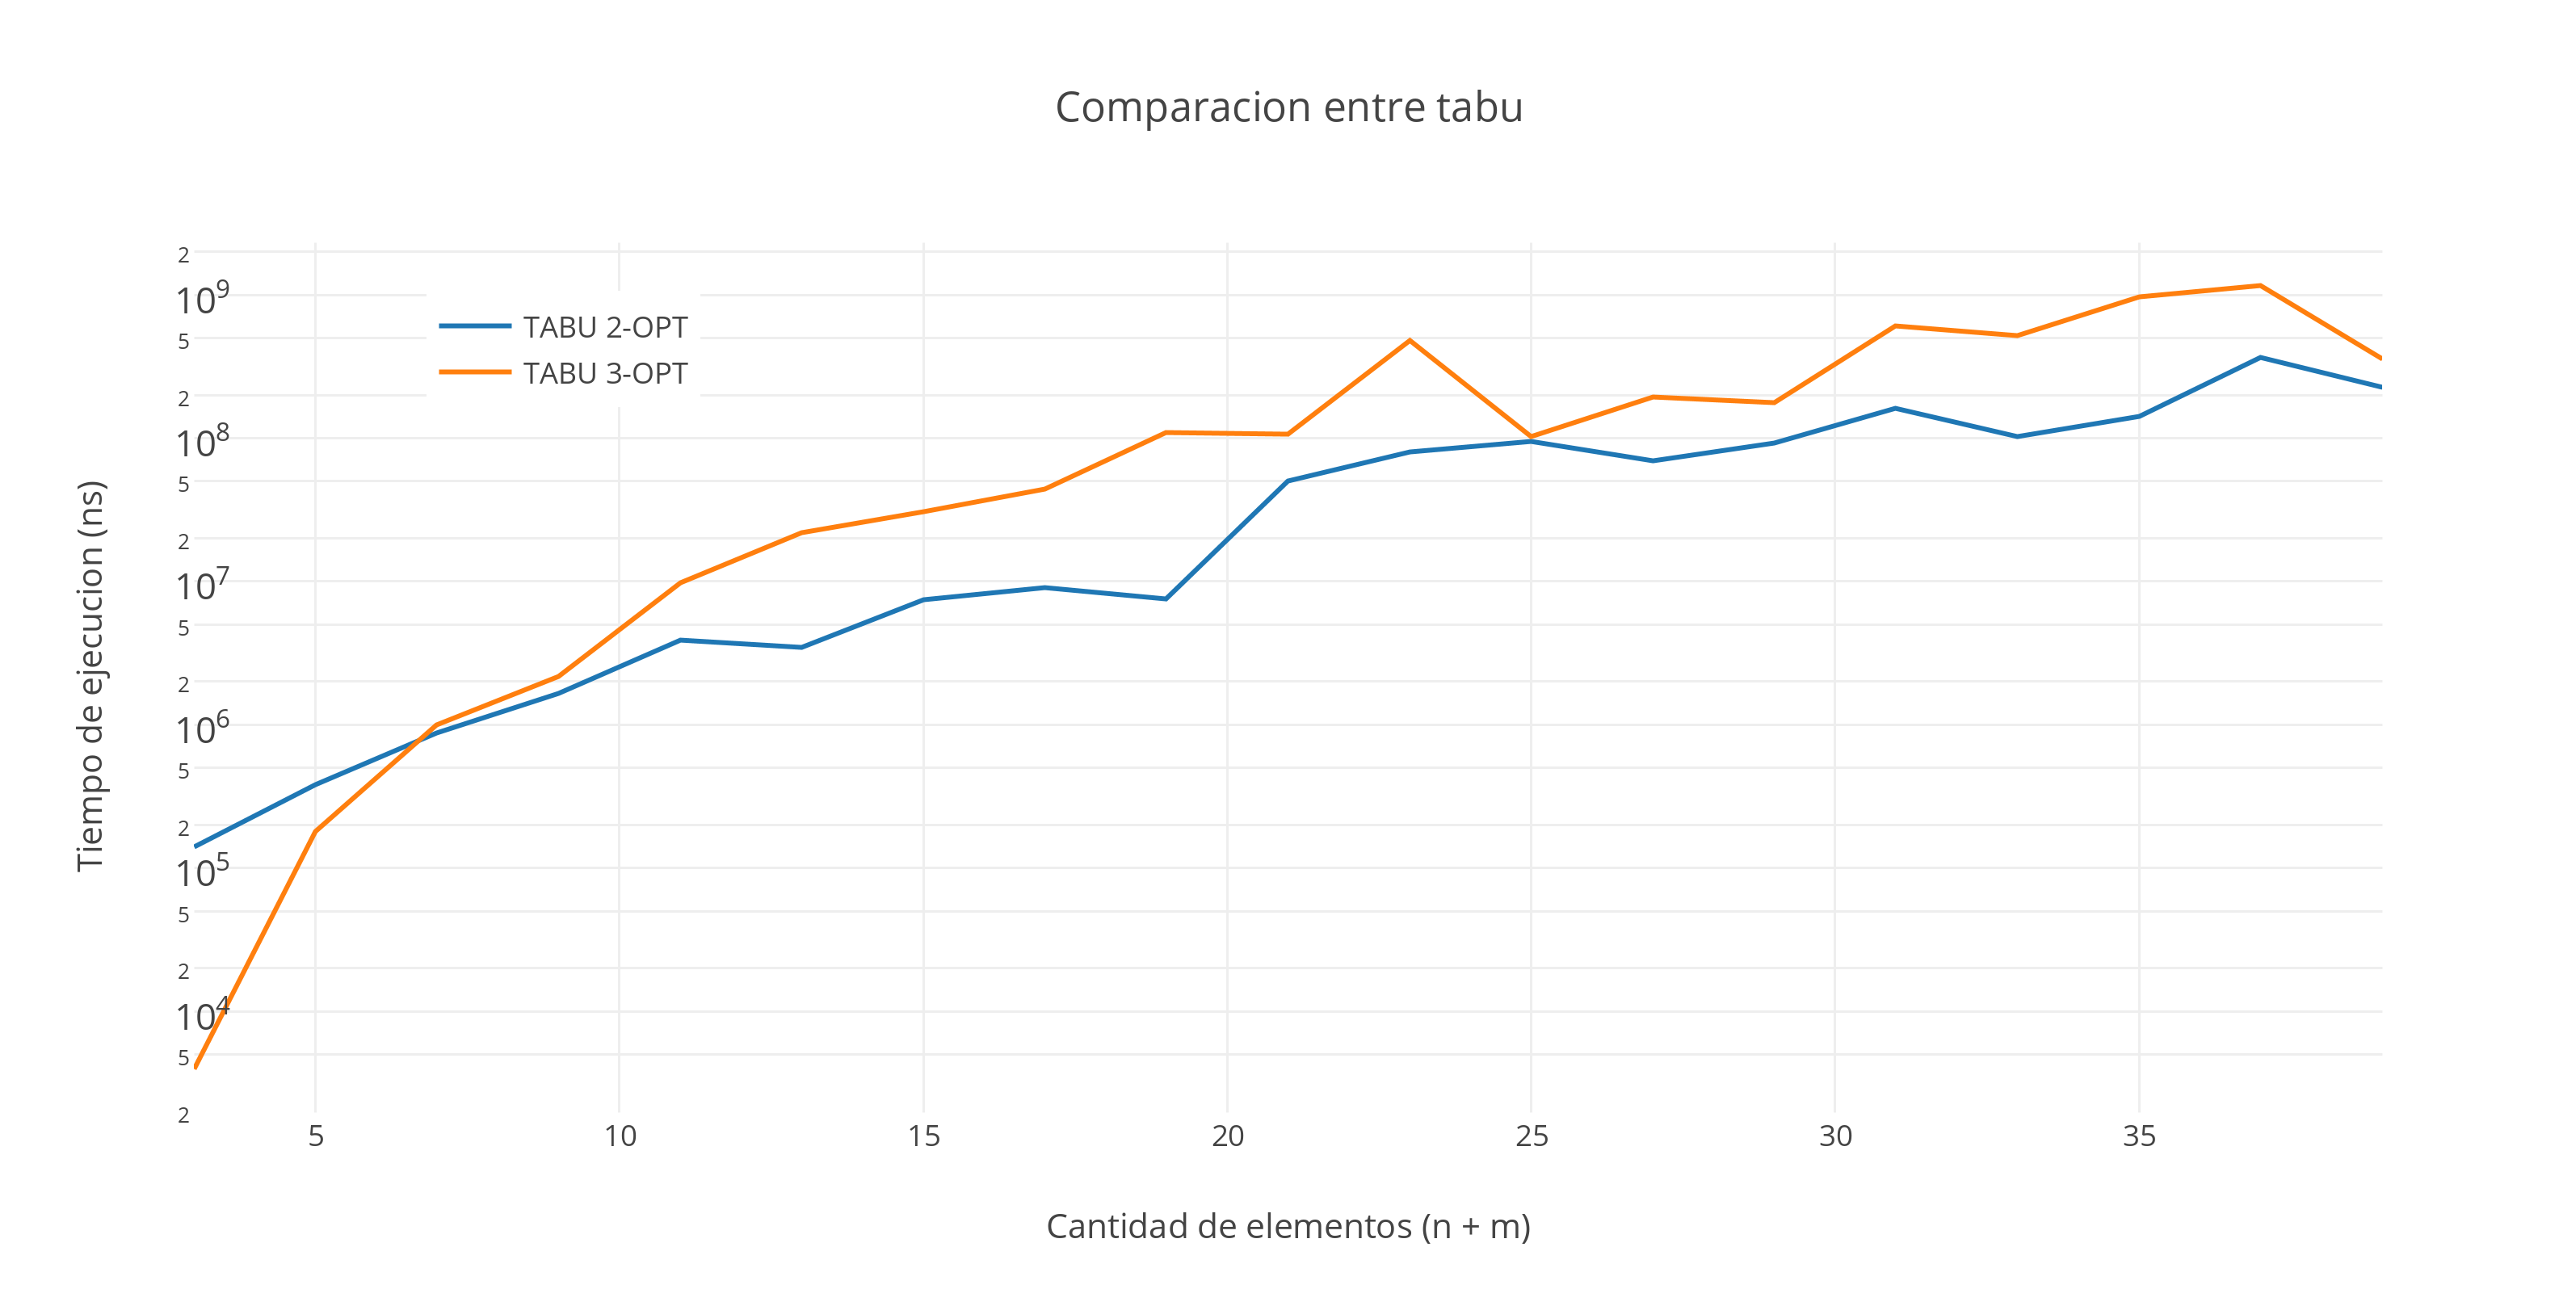
\includegraphics[scale=0.5]{./EJ4/comparaciongym01.png}\\
 {            \textit{Gráfico \ 4.6 - Tabu 2-OPT vs Tabu 3-OPT sobre Familia 4}}
  \end{center}
  \vspace*{0.3cm}

Se pudo observar como la heur\'istica Tabu 2-OPT mejoro considerablemente las soluciones para 2-OPT, mientras que en relaci\'on a Tabu 3-OPT y 3-OPT las soluciones obtenidas fueron similares. Teniendo en cuenta adem\'as, que para esta \'ultima el tiempo insumido fue considerablemente mayor que la b\'usqueda local.
Por lo tanto, para esta familia puntualmente, a la hora de elegir una entre los dos Tabu, ser\'a m\'as eficiente en relaci\'on tiempo - calidad de soluci\'on la Tabu 2-OPT.


\subsubsection*{Familia 6}

Como enunciamos anteriormente esta familia tiene como caracter\'istica principal tener pokeparadas a ambos lados de gimnasios, generando que el resultado de la heur\'istica golosa de una soluci\'on muy alejada de la \'optima, por esta raz\'on luego de haber realizado nuevas heur\'isticas de b\'usquedas locales, puntualmente 2-OPT y 3-OPT, pudimos observar que se vio mejorada la soluci\'on. 

Procederemos a ver, si con las nuevas heuristicas implementadas Tabu 2-OPT y 3-OPT la solucion que obtenemos se acerca o iguala a la \'optima.

Veamos un ejemplo de como se mejora el camino obtenido por el goloso al utilizar Tabu 2-OPT y Tabu 3-OPT:

\vspace*{0.3cm} \vspace*{0.3cm}
  \begin{center}
 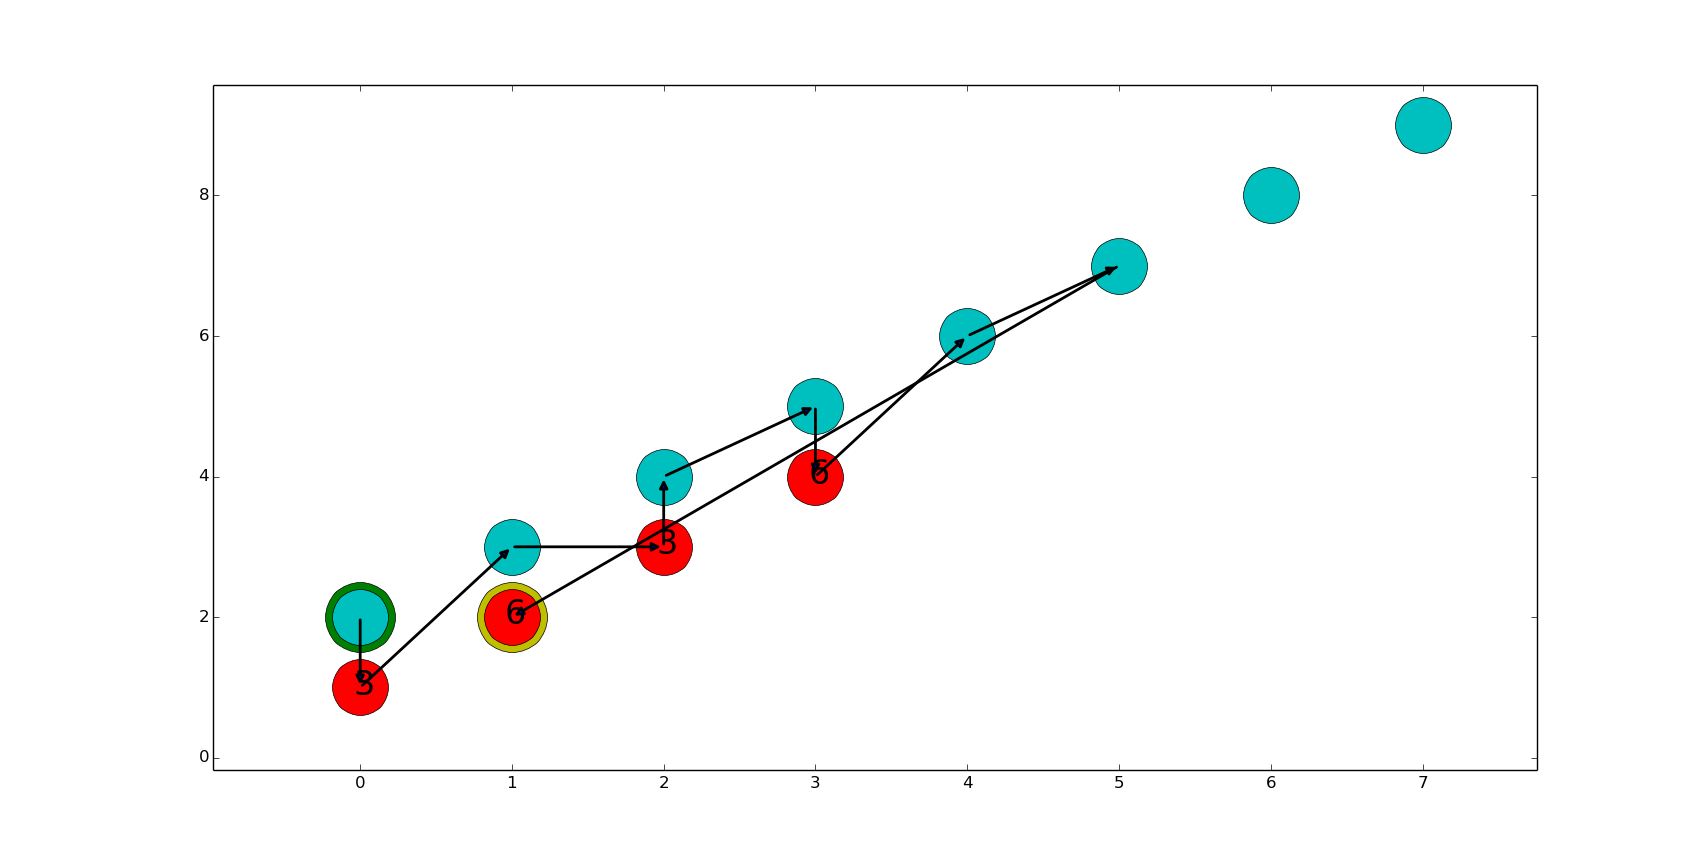
\includegraphics[scale=0.3]{./EJ4/fam6goloso.png}\\
 {            \textit{Soluci\'on Golosa}}
  \end{center}
  \vspace*{0.3cm}

\vspace*{0.3cm} \vspace*{0.3cm}
  \begin{center}
 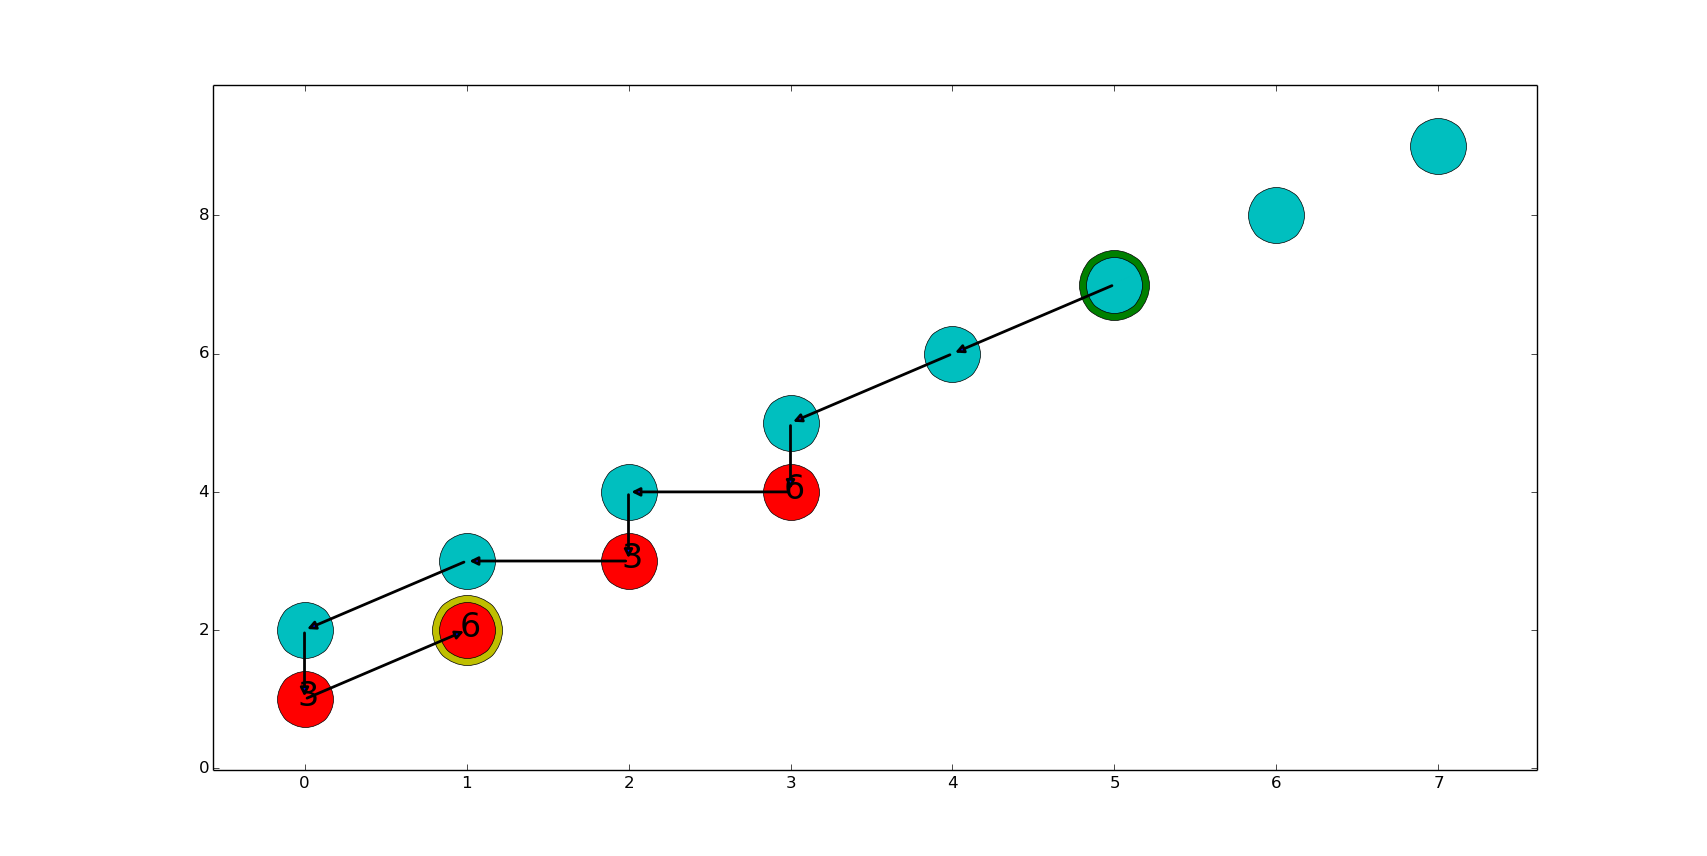
\includegraphics[scale=0.3]{./EJ4/fam62opt.png}\\
 {            \textit{Soluci\'on TABU 2-OPT}}
  \end{center}
  \vspace*{0.3cm}

\vspace*{0.3cm} \vspace*{0.3cm}
  \begin{center}
 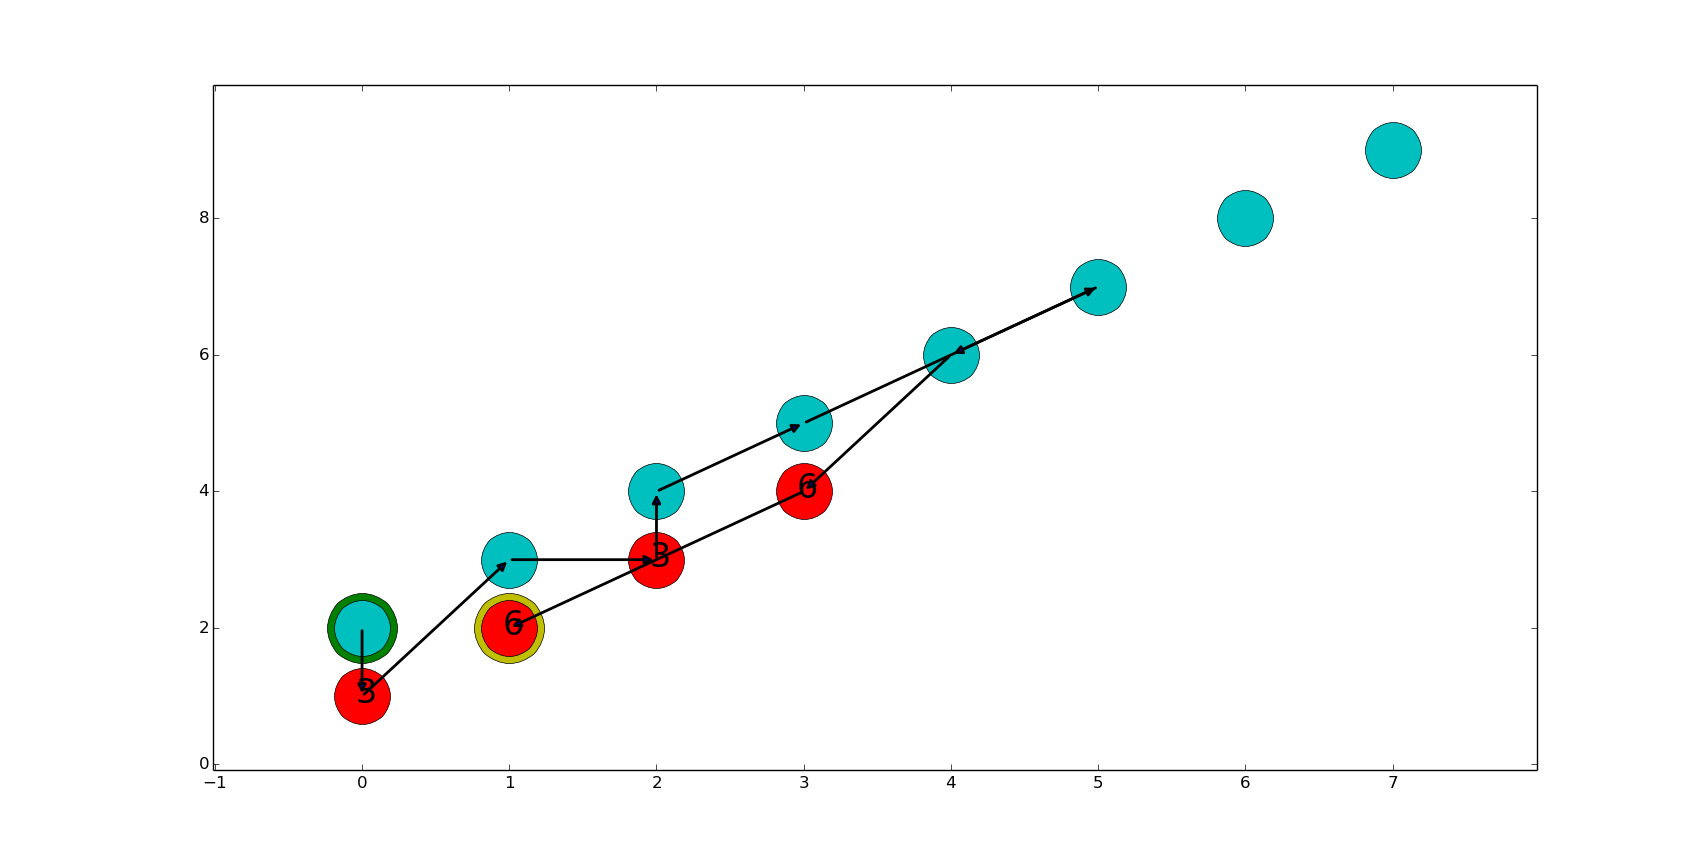
\includegraphics[scale=0.3]{./EJ4/fam63opt.png}\\
 {            \textit{Soluci\'on TABU 3-OPT}}
  \end{center}
  \vspace*{0.3cm}

Luego de haber ejemplificado una instancia posible queremos ver como se comporta Tabu 2-OPT con respecto a la heur\'istica de busqueda local 2-OPT:

\vspace*{0.3cm} \vspace*{0.3cm}
  \begin{center}
 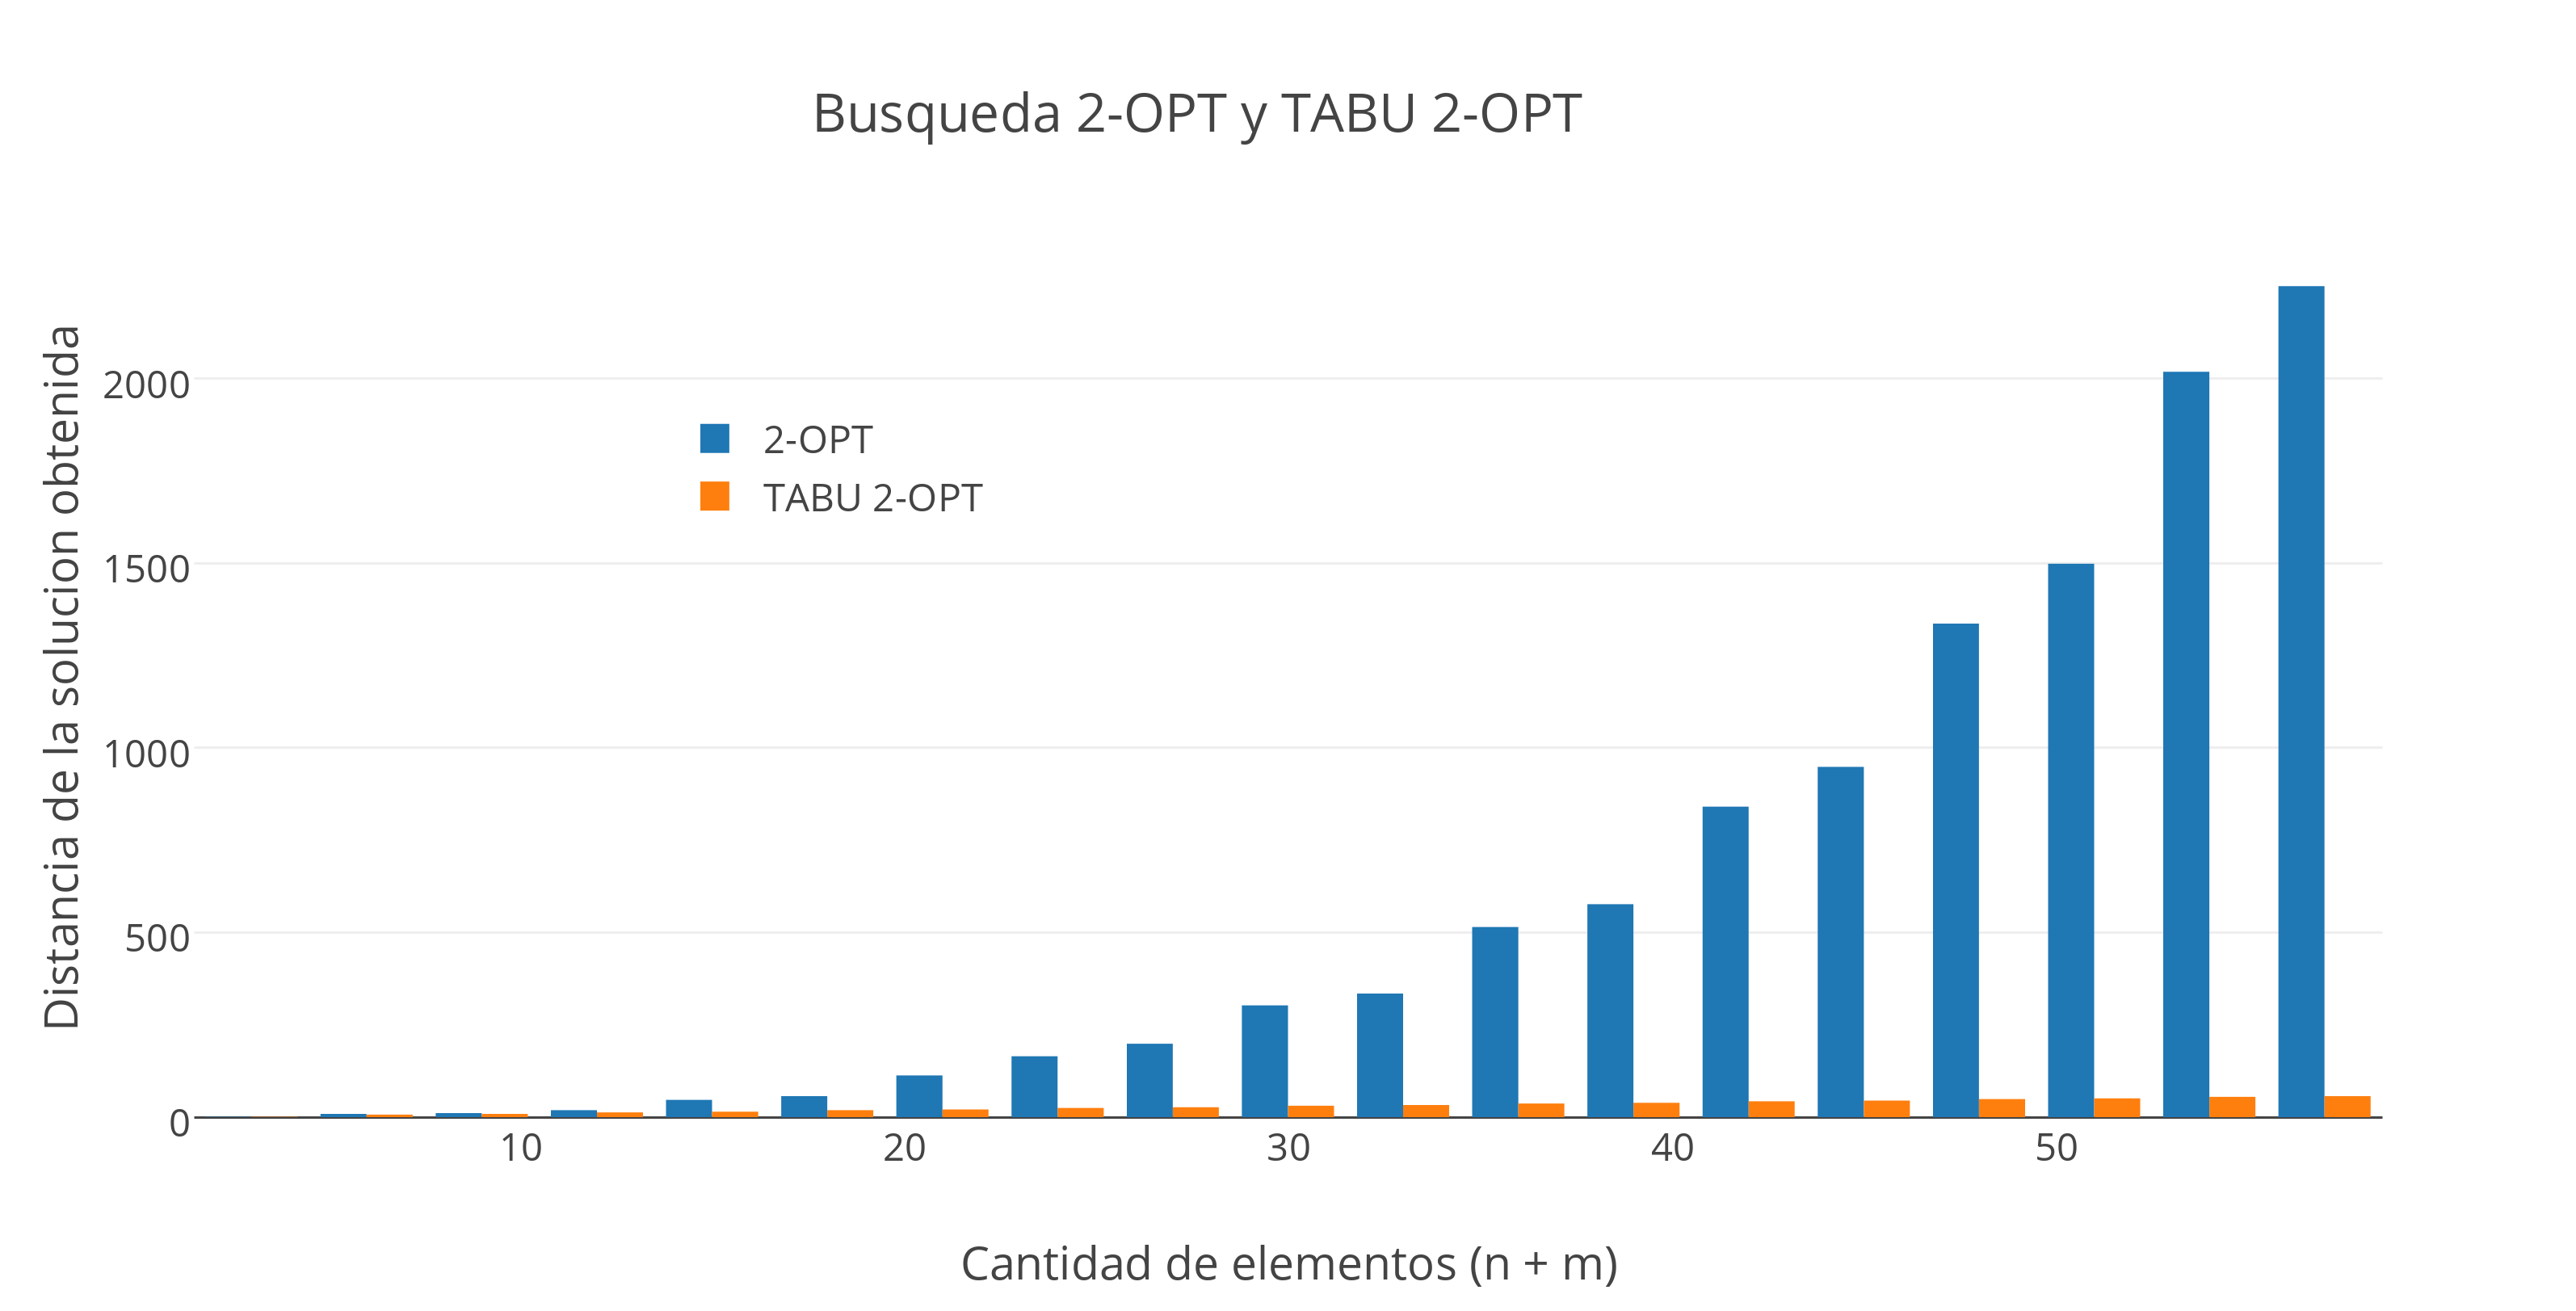
\includegraphics[scale=0.5]{./EJ4/comparativosinorden2opt.png}\\
 {            \textit{Gráfico \ 4.7 - 2-OPT vs Tabu 2-OPT sobre Familia 6}}
  \end{center}
  \vspace*{0.3cm}

\vspace*{0.3cm} \vspace*{0.3cm}
  \begin{center}
 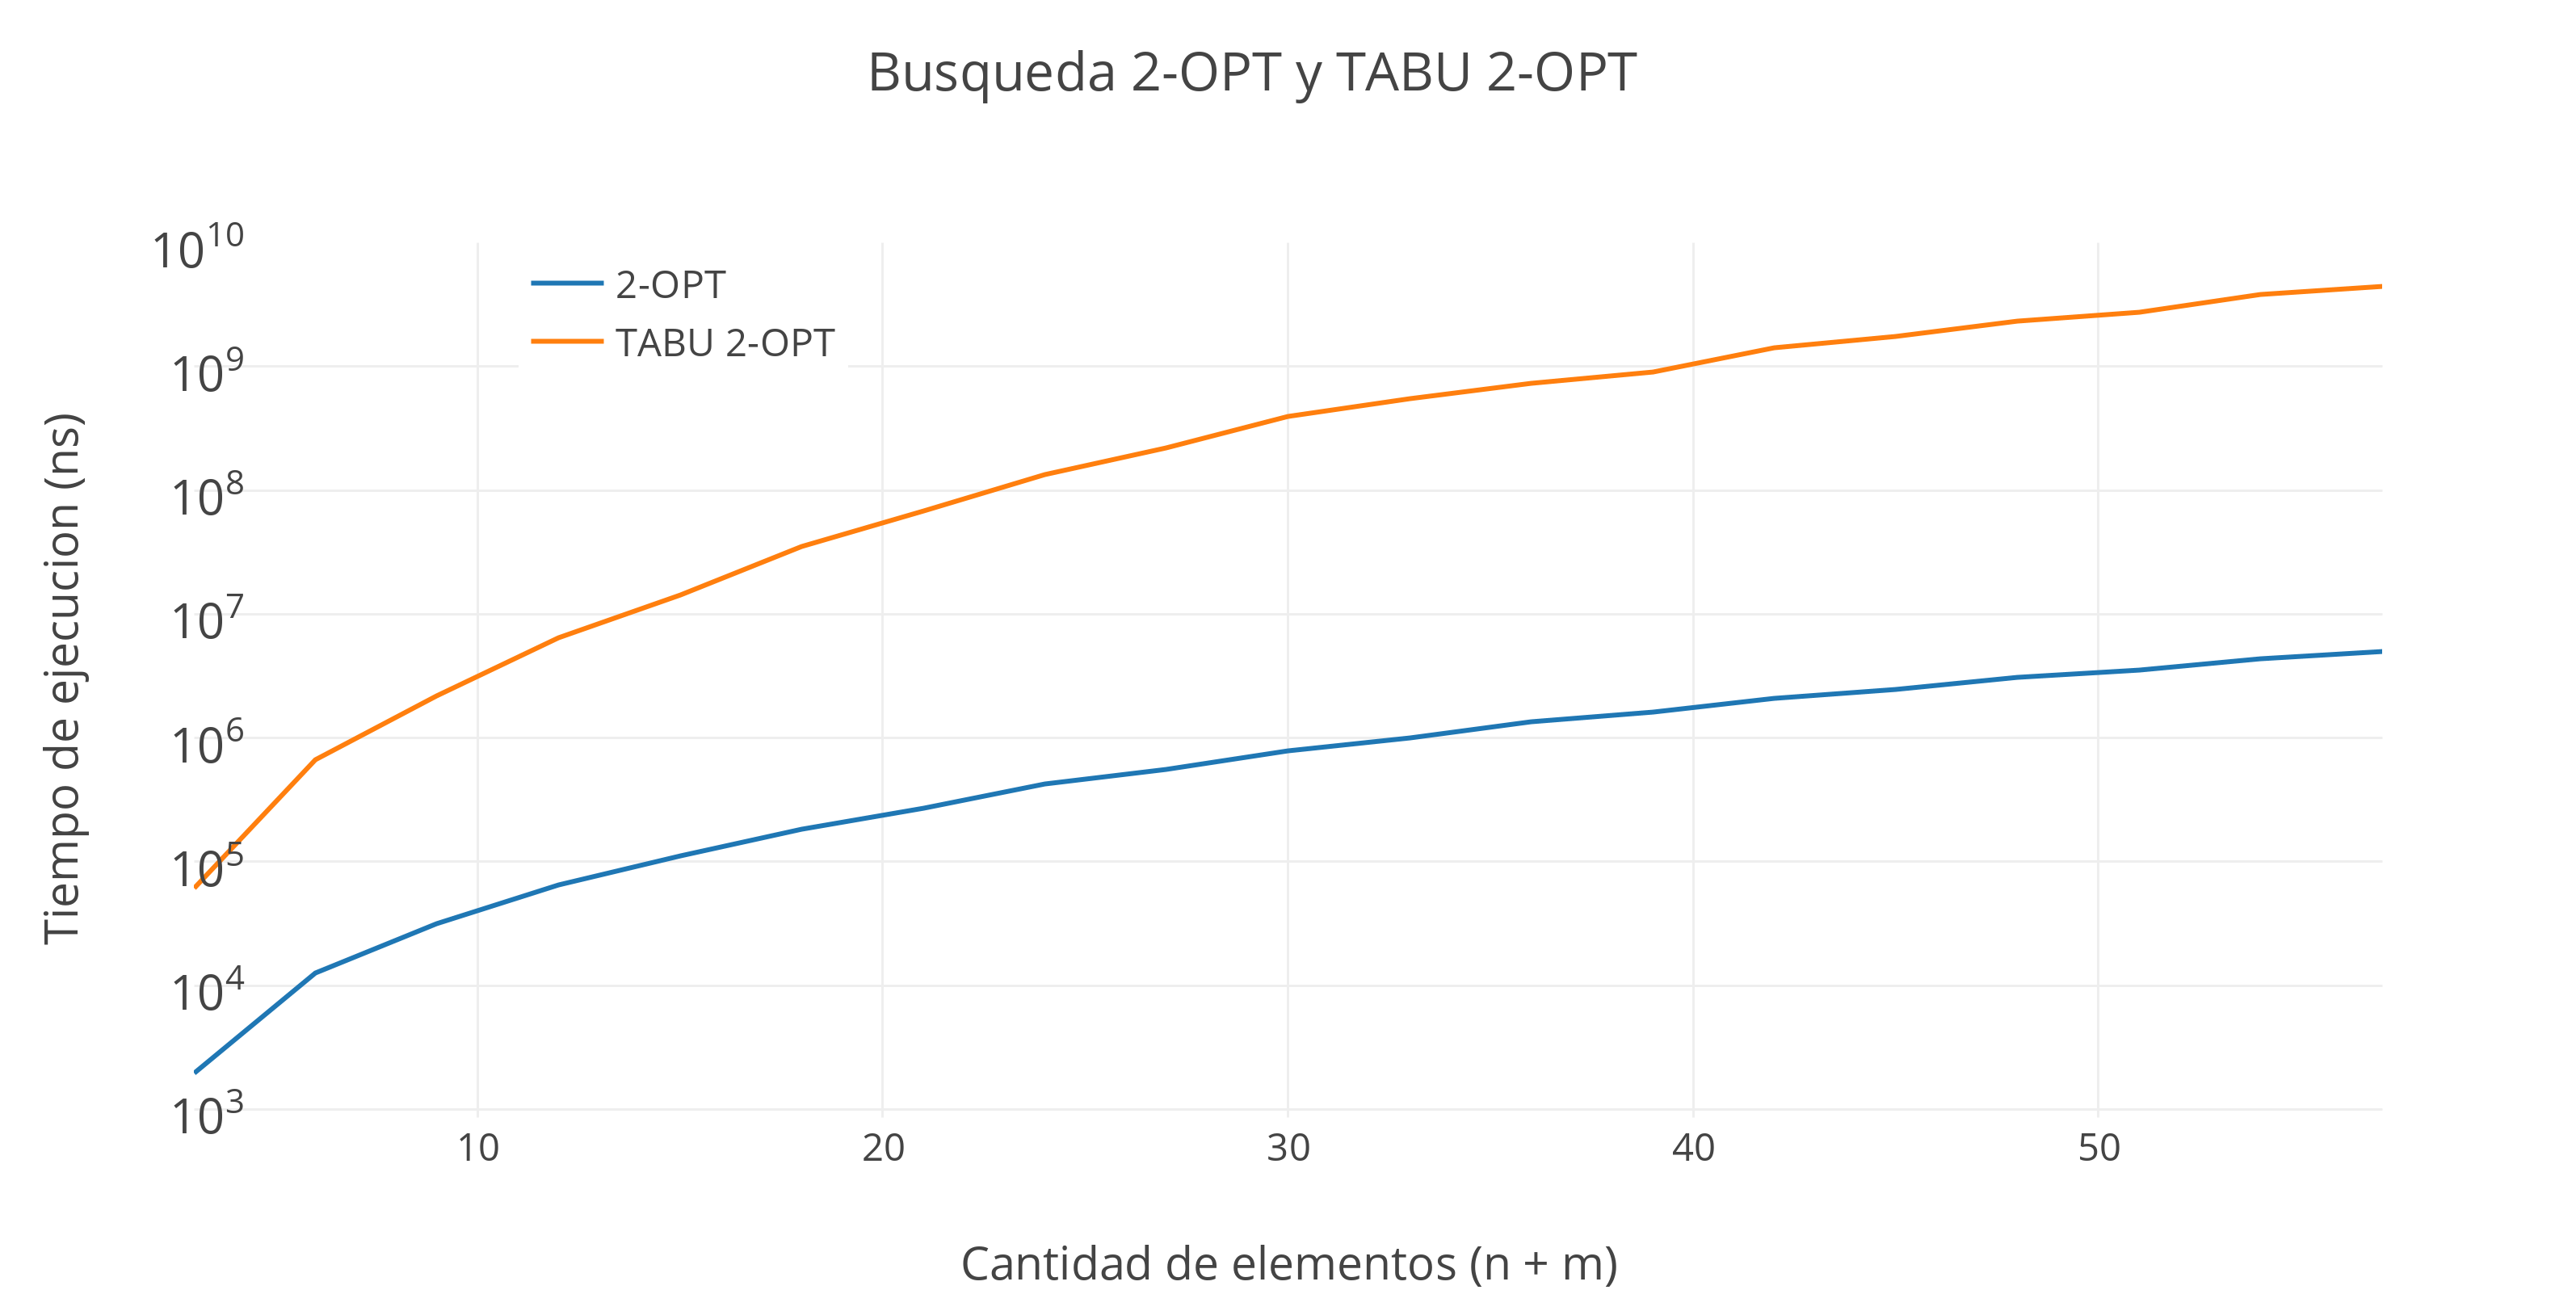
\includegraphics[scale=0.5]{./EJ4/medicion2optsinorden.png}\\
 {            \textit{Gráfico \ 4.8 - 2-OPT vs Tabu 2-OPT sobre Familia 6}}
  \end{center}
  \vspace*{0.3cm}

Luego, para 3-OPT:

\vspace*{0.3cm} \vspace*{0.3cm}
  \begin{center}
 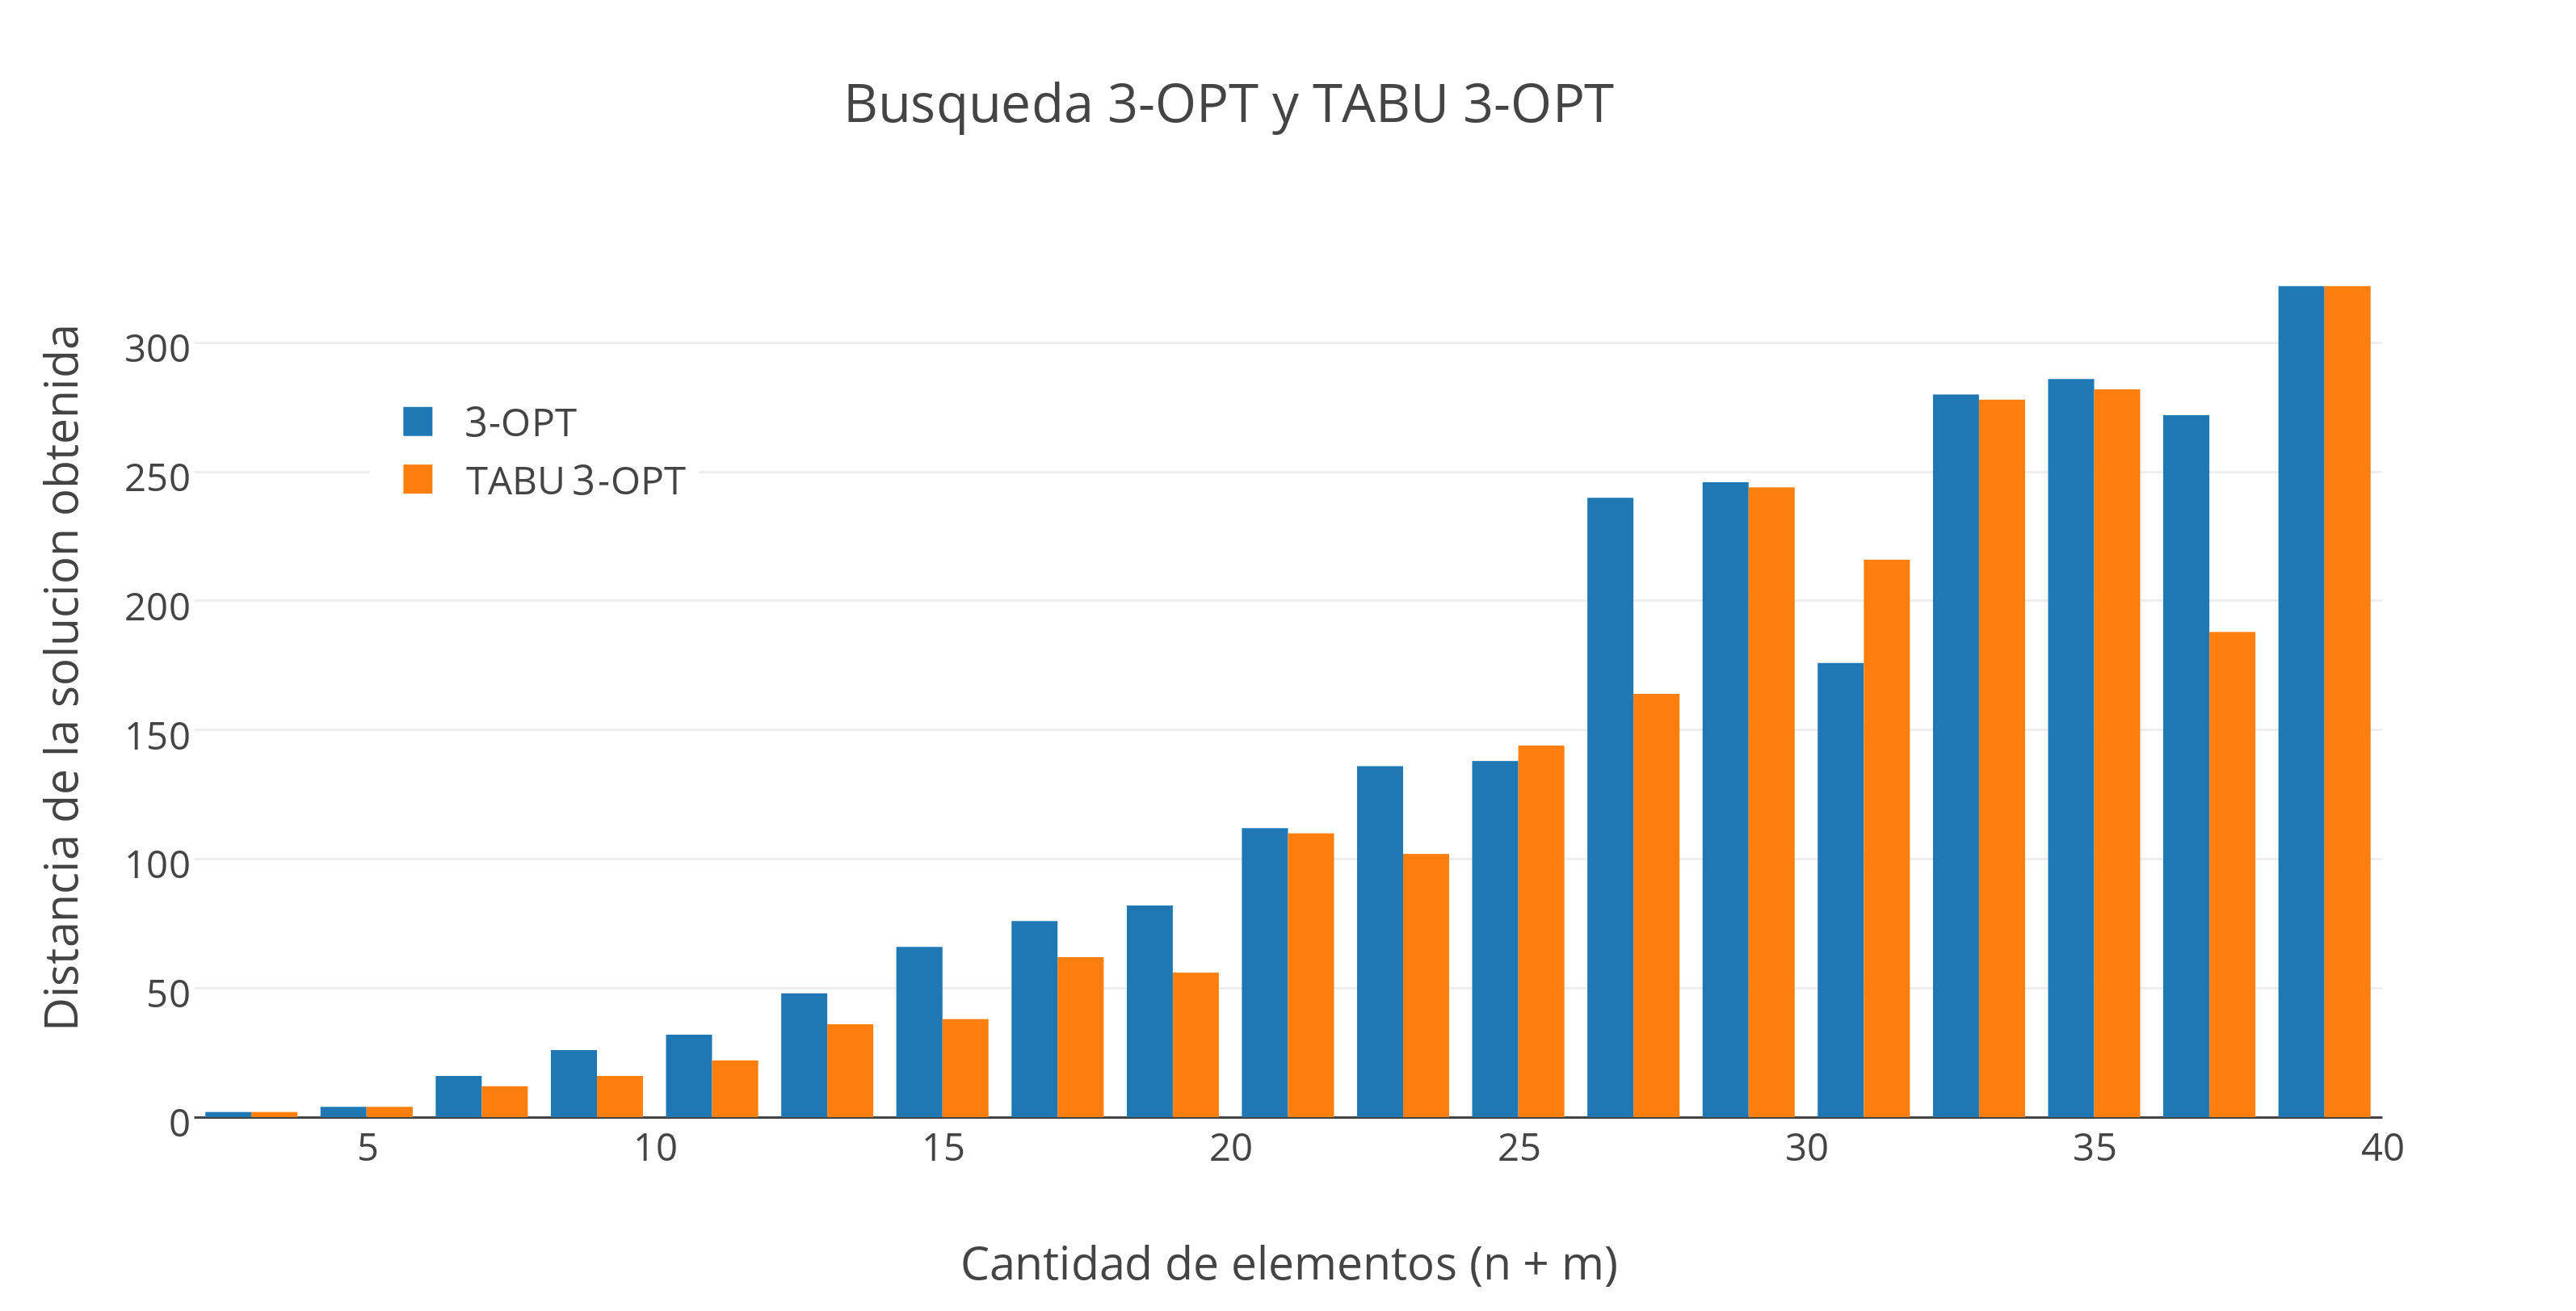
\includegraphics[scale=0.5]{./EJ4/comparativogym03opt.png}\\
 {            \textit{Gráfico \ 4.9 - 3-OPT vs Tabu 3-OPT sobre Familia 6}}
  \end{center}
  \vspace*{0.3cm}

\vspace*{0.3cm} \vspace*{0.3cm}
  \begin{center}
 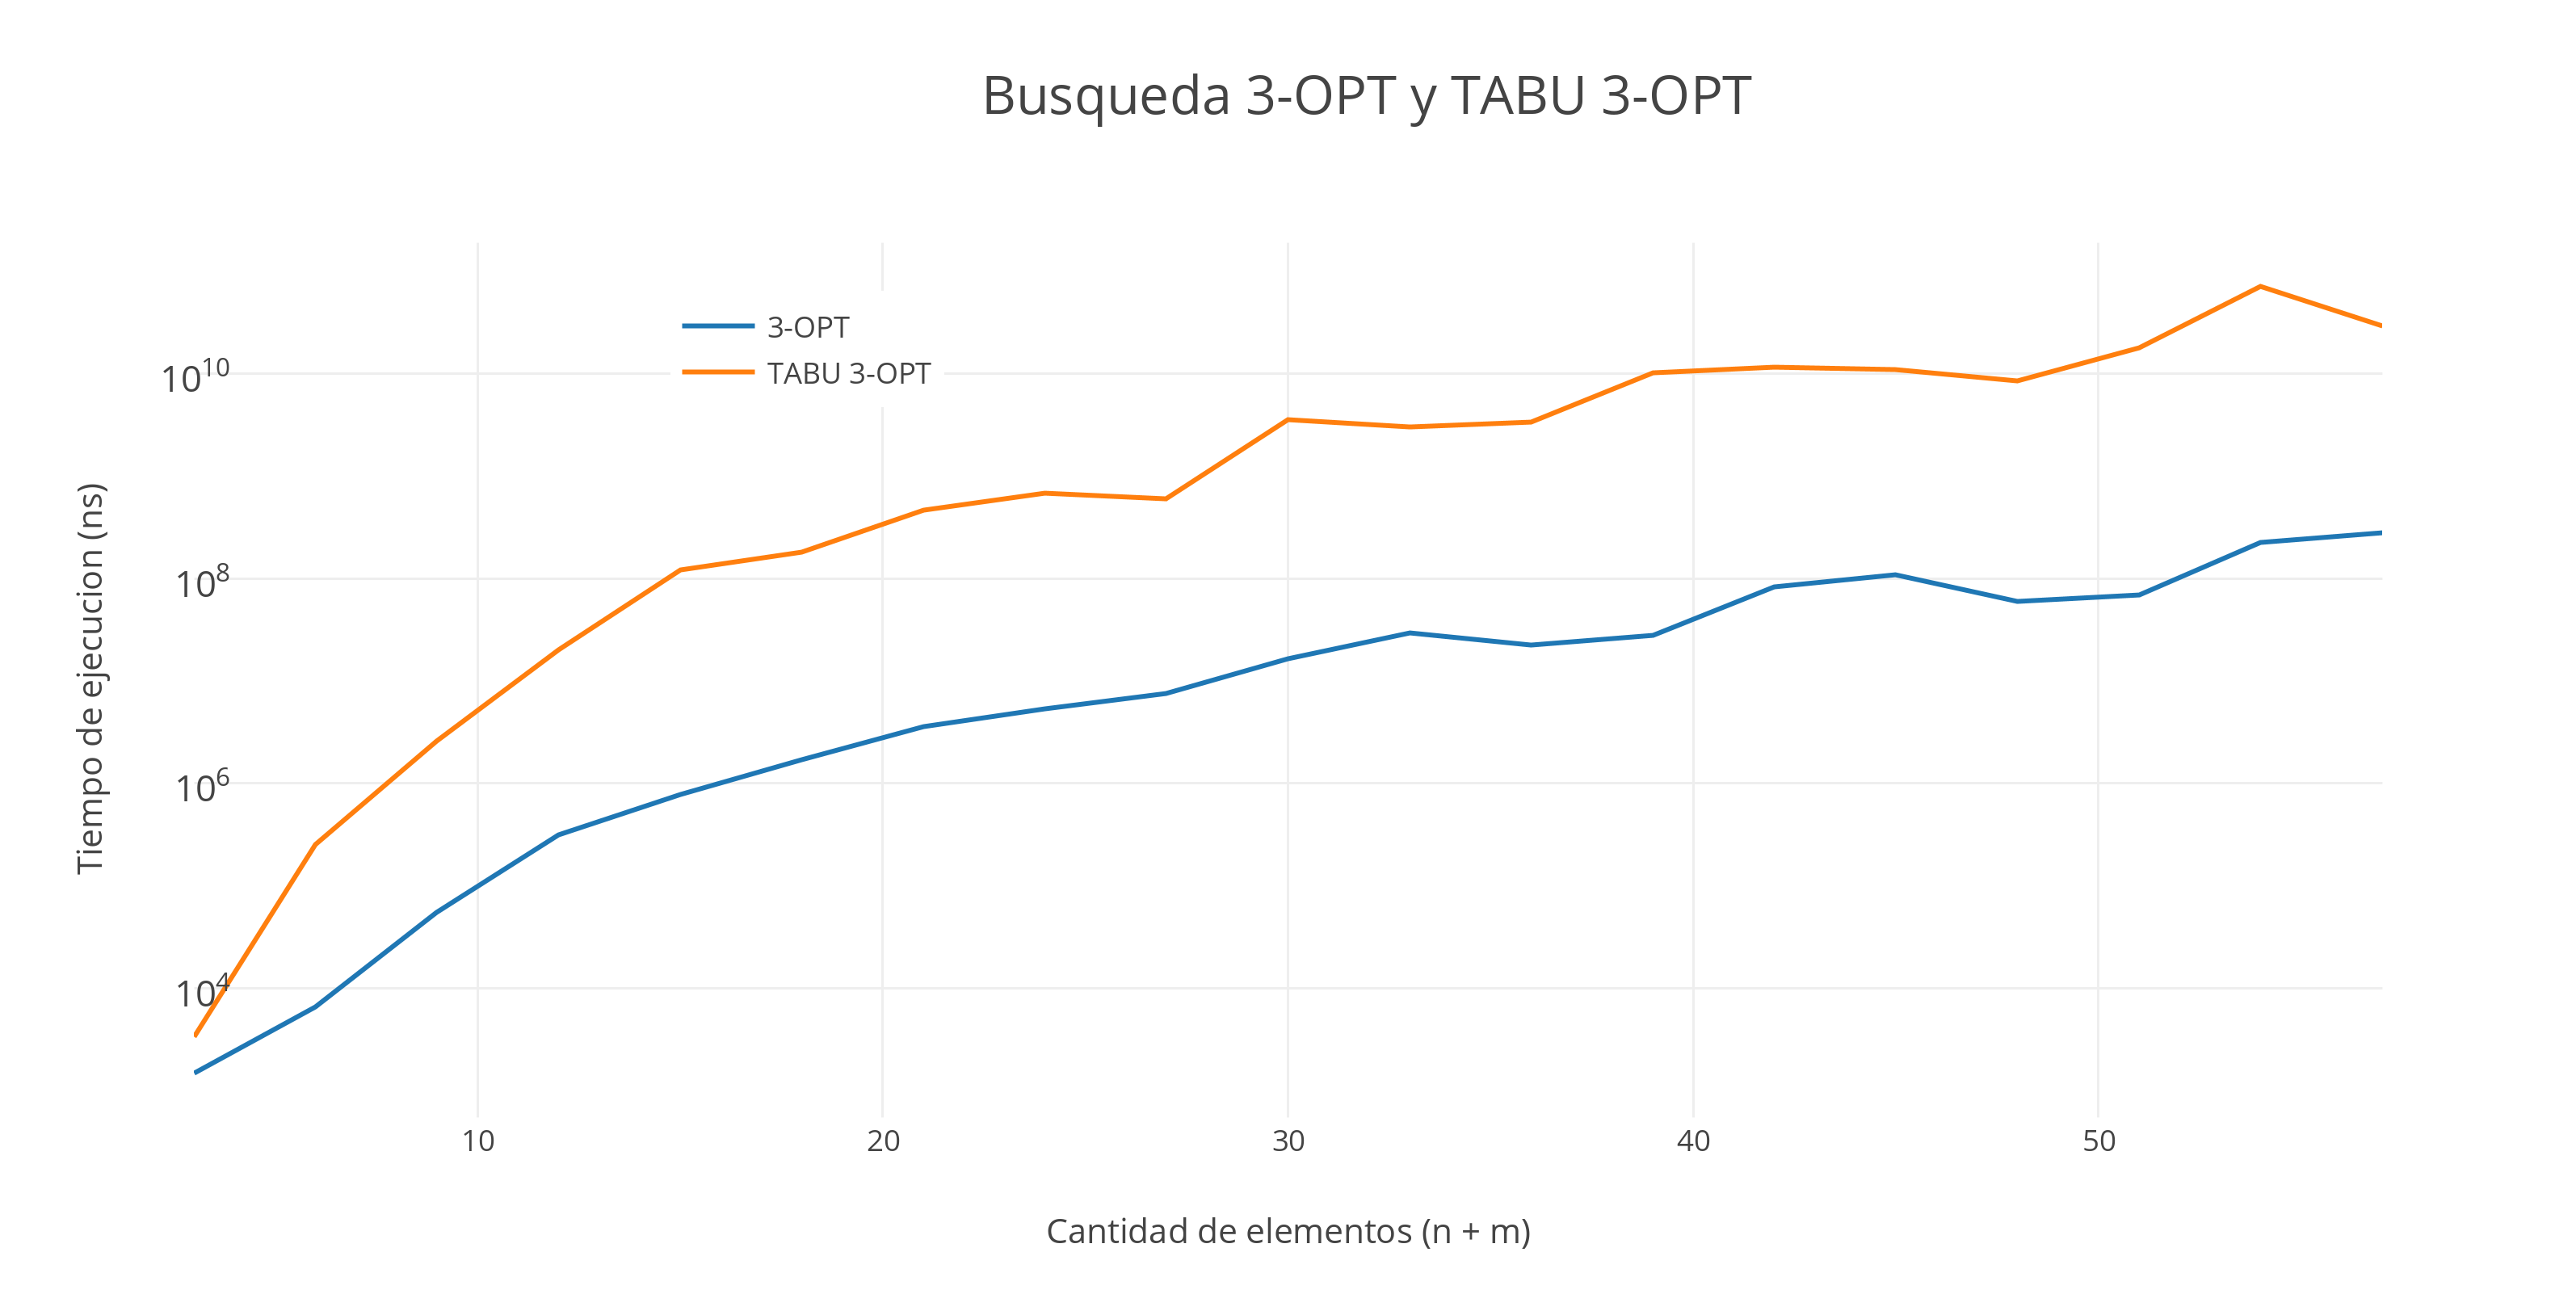
\includegraphics[scale=0.5]{./EJ4/medicion3optsinorden.png}\\
 {            \textit{Gráfico \ 4.10 - 3-OPT vs Tabu 3-OPT sobre Familia 6}}
  \end{center}
  \vspace*{0.3cm}
  
Habiendo chequeado dichos experimentos, pudimos observar que utilizando Tabu 2-OPT mejoramos considerablemente la soluci\'on obtenida por 2-OPT. A pesar de tener en cuenta que, en la medici\'on de tiempo insumido el tabu tarda m\'as, la calidad de soluci\'on obtenida es hasta 10 veces mejor que en la b\'usqueda, es por esto que, para esta familia puntual es preferible trabajar con Tabu 2-OPT que con la b\'usqueda en cuesti\'on. 
Por otro lado, el otro Tabu, en ves de mejorar la soluci\'on en muchos casos nos otorga una soluci\'on inferior a la que ya ten\'iamos.
  
Comparando las soluciones de cada version de tabú search podemos observar lo siguiente:

\vspace*{0.3cm} \vspace*{0.3cm}
  \begin{center}
 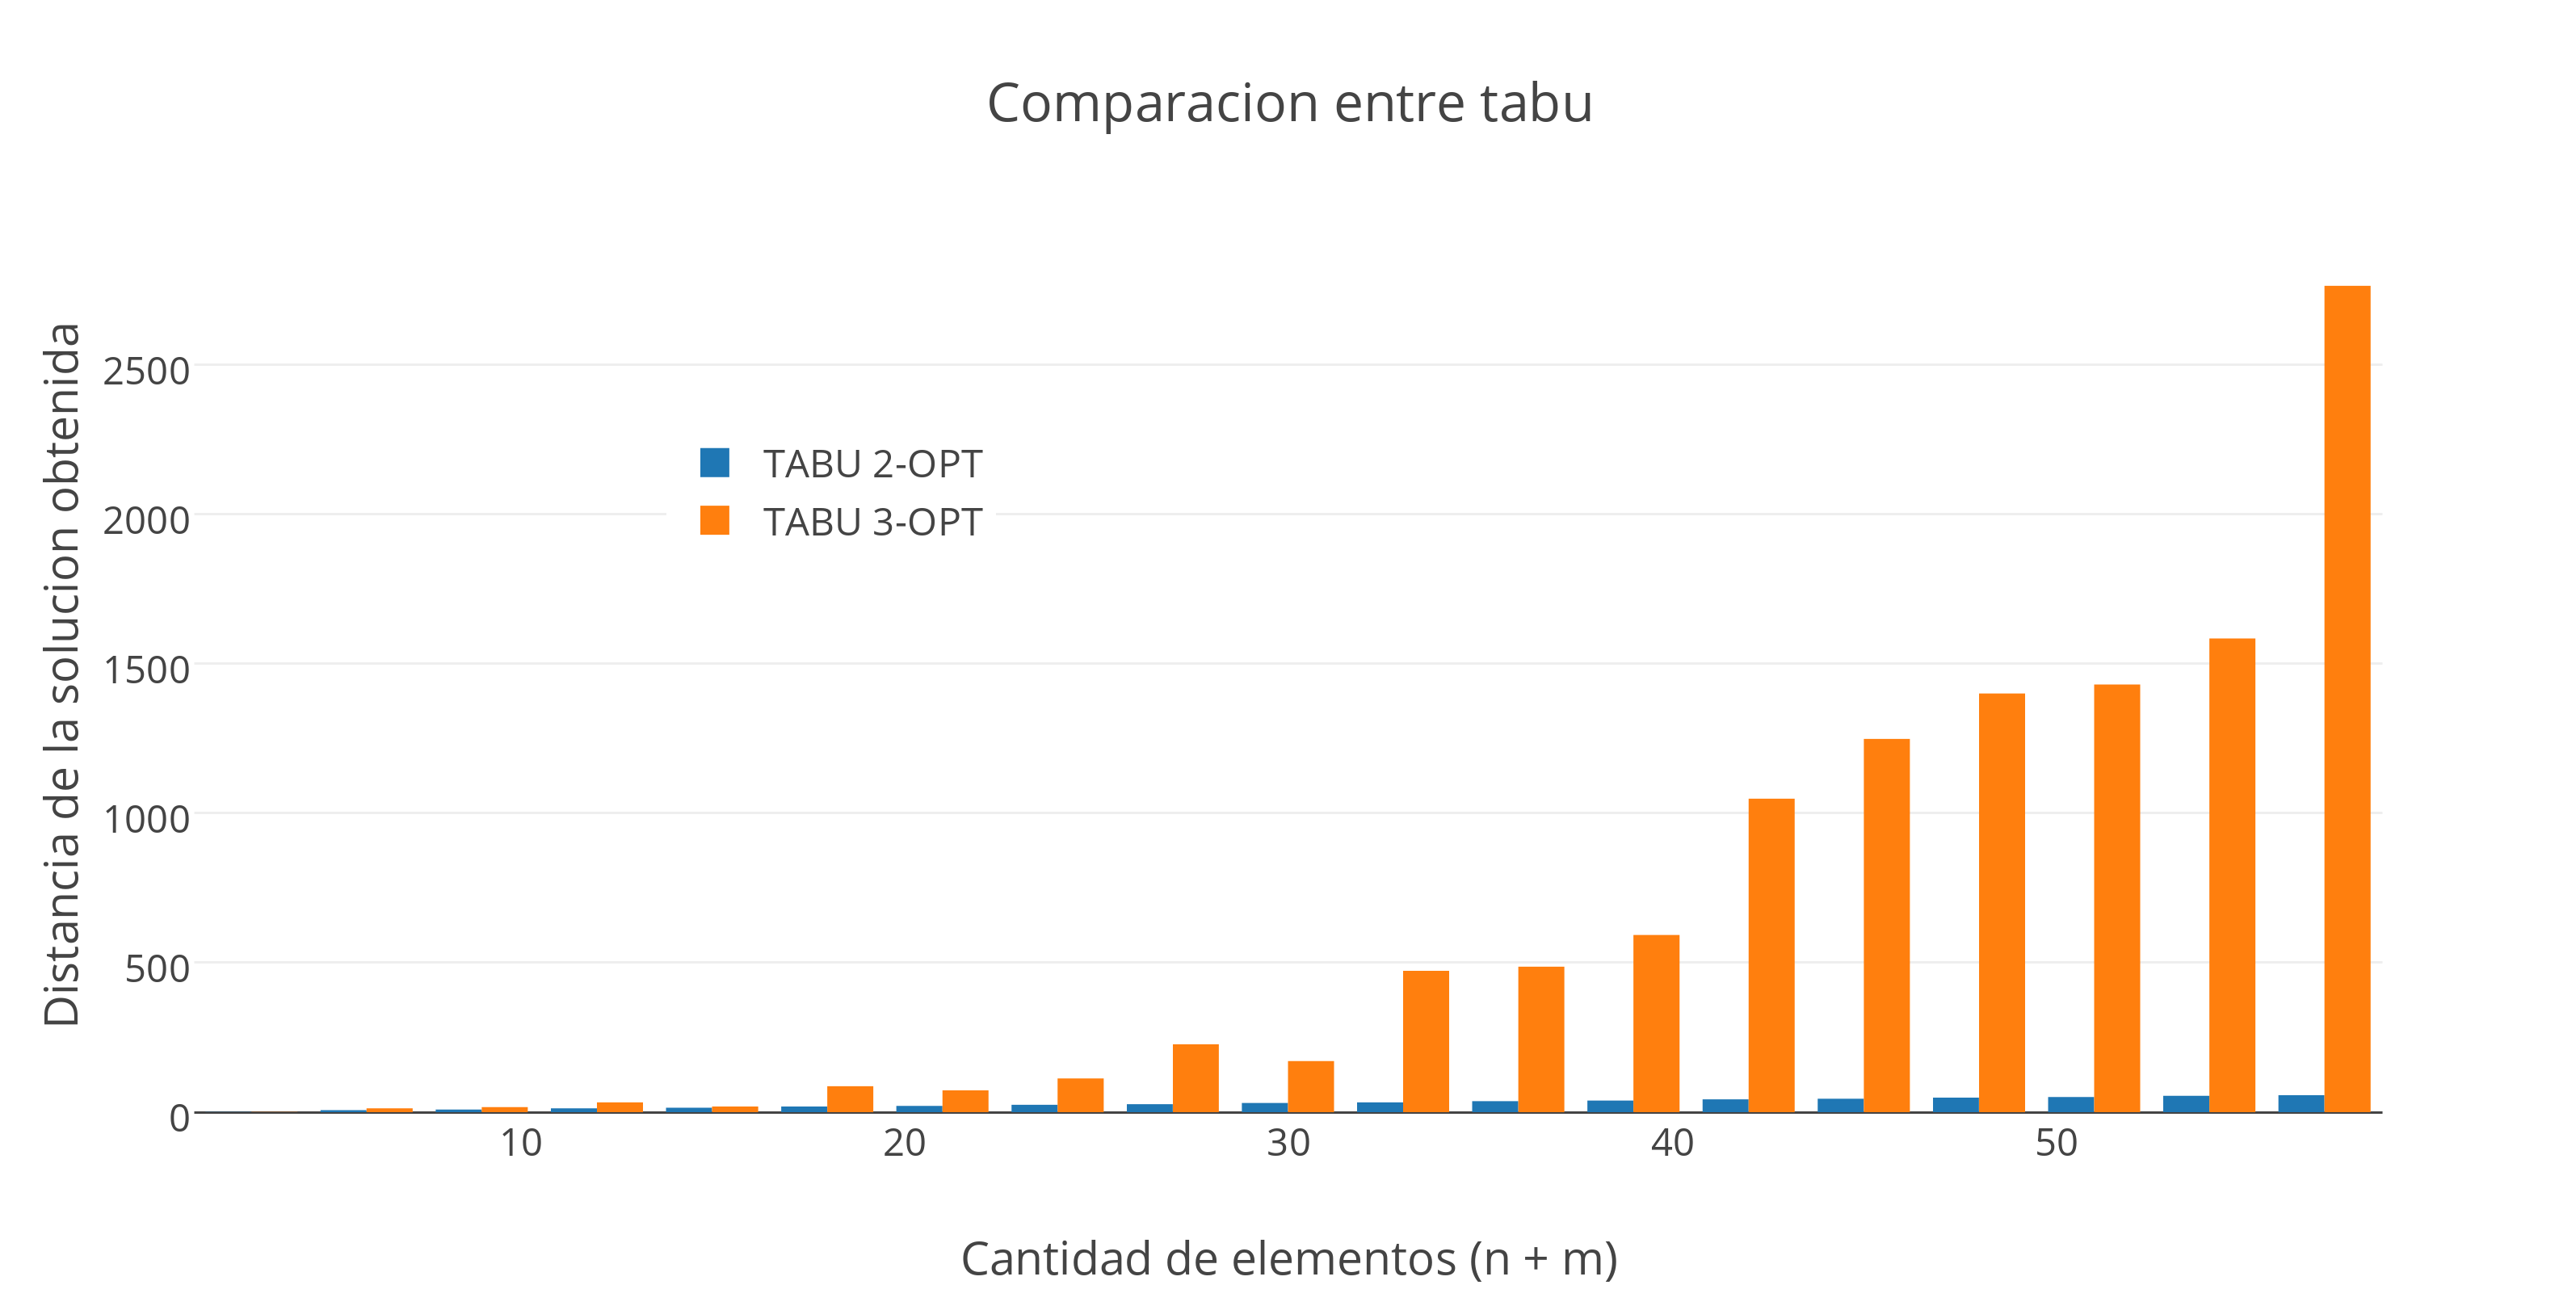
\includegraphics[scale=0.5]{./EJ4/comparativosinorden.png}\\
 {            \textit{Gráfico \ 4.11 - Tabu 2-OPT vs Tabu 3-OPT sobre Familia 6}}
  \end{center}
  \vspace*{0.3cm}

En cuanto a tiempo insumido vemos lo siguiente:

\vspace*{0.3cm} \vspace*{0.3cm}
  \begin{center}
 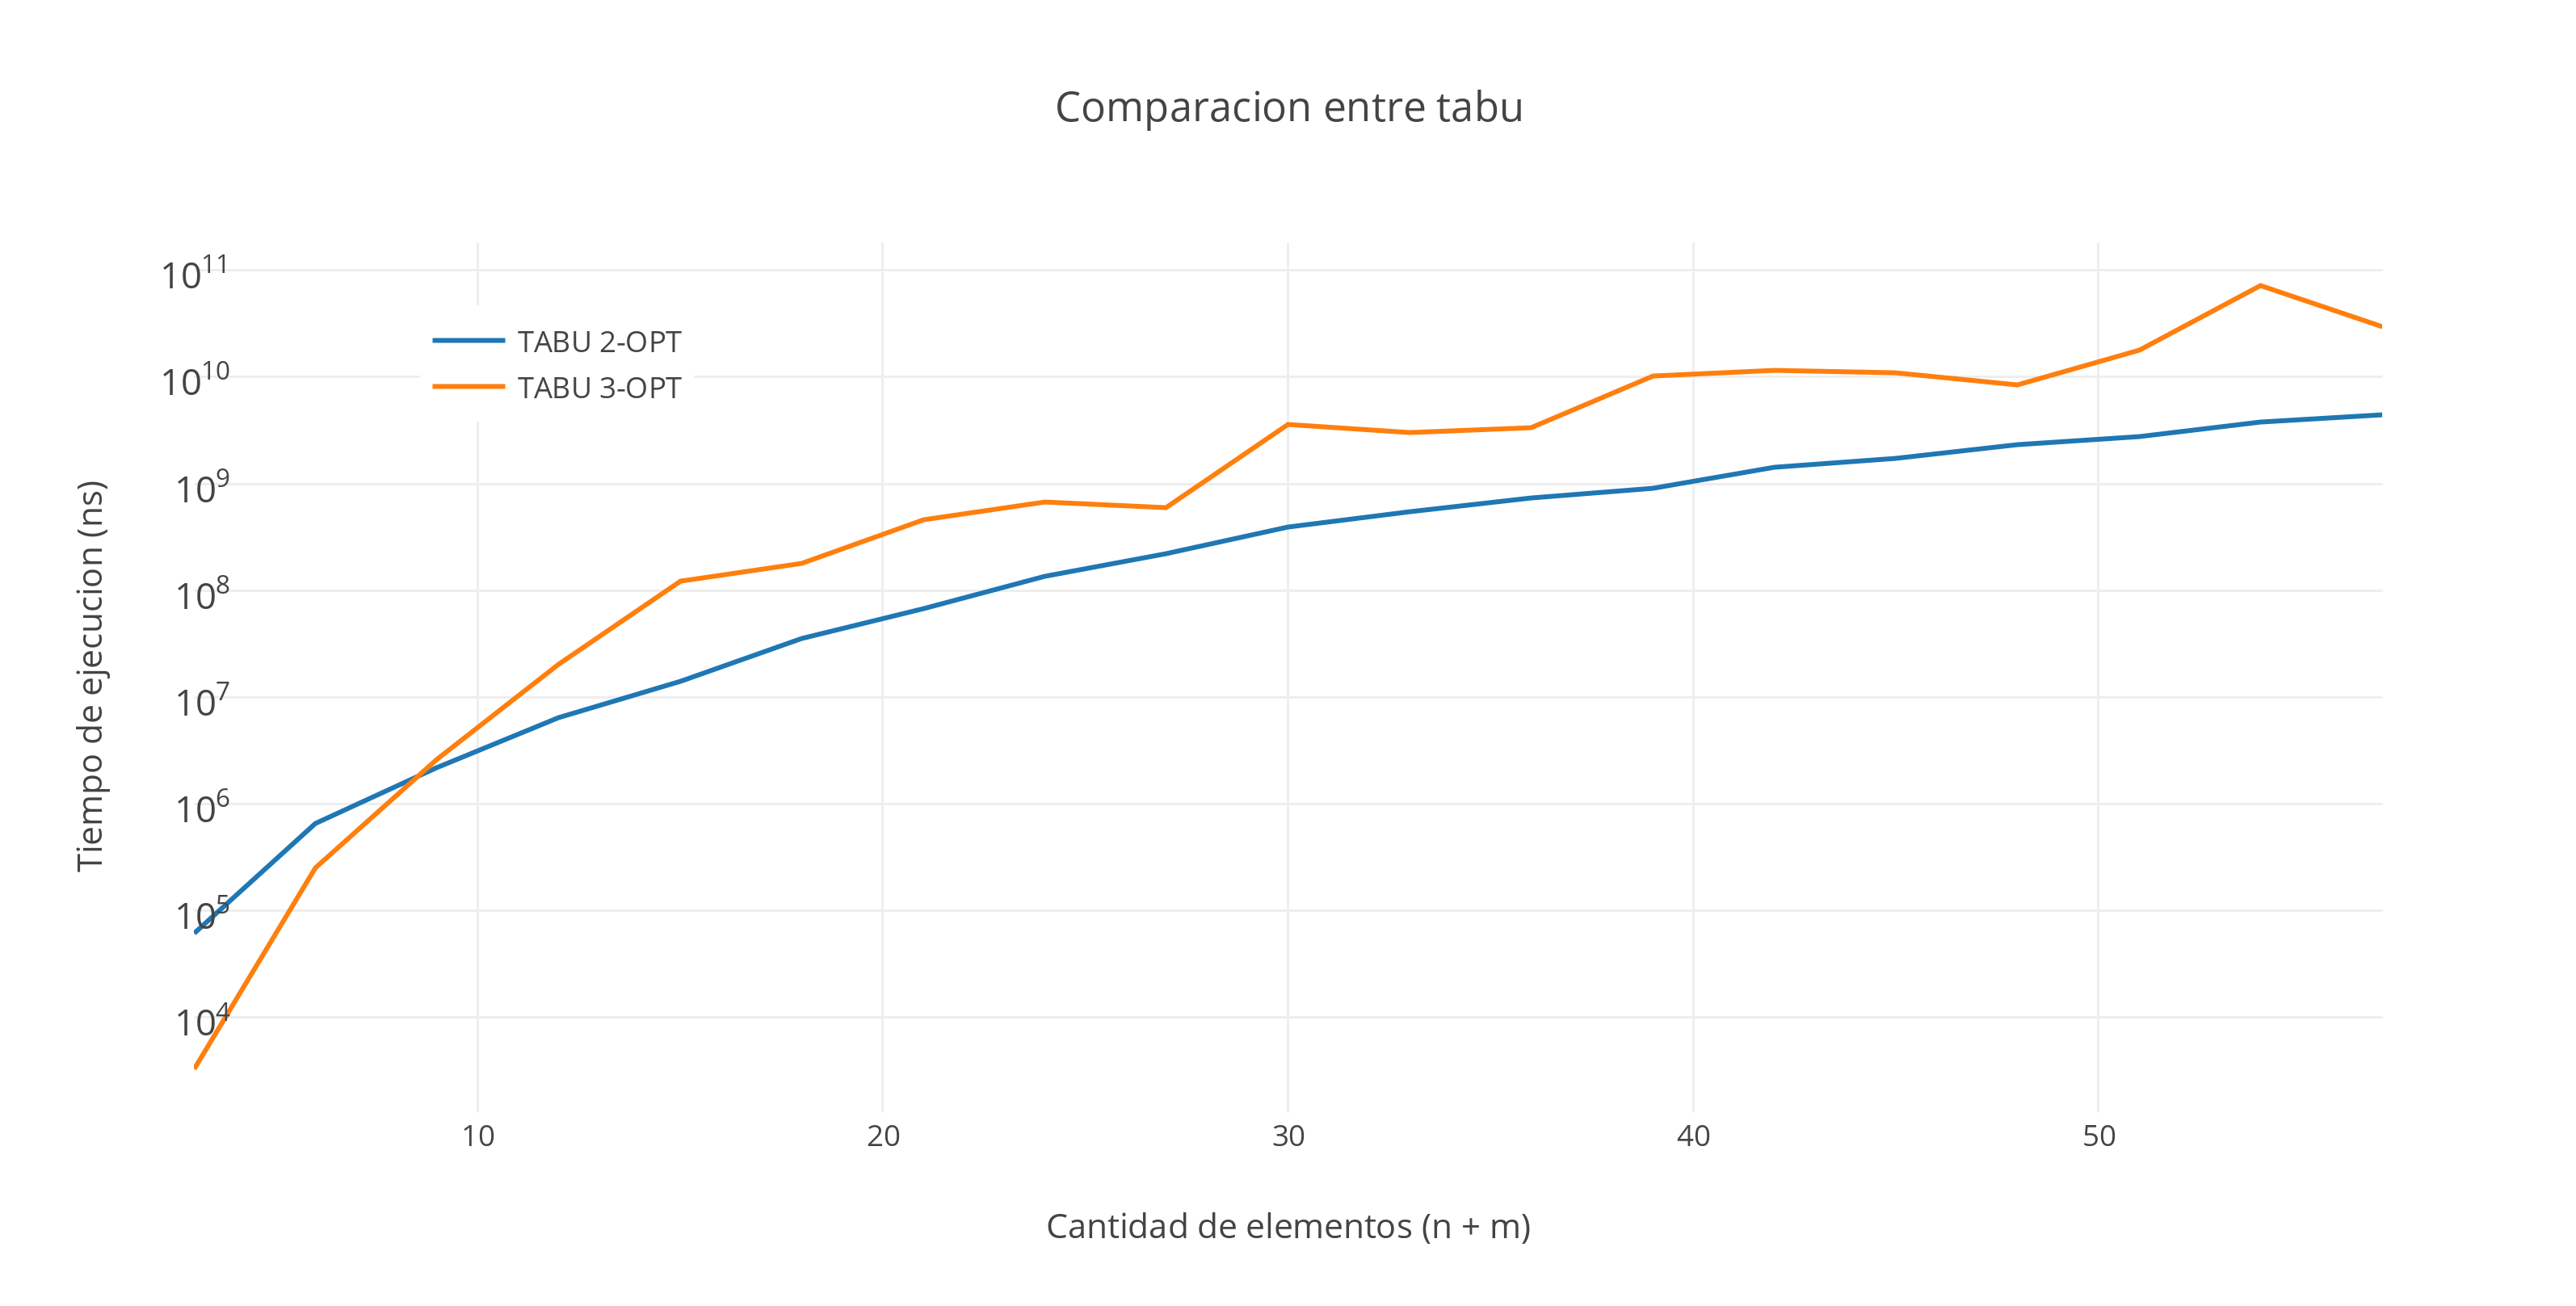
\includegraphics[scale=0.5]{./EJ4/comparacionsinorden1.png}\\
 {            \textit{Gráfico \ 4.12 - Tabu 2-OPT vs Tabu 3-OPT sobre Familia 6}}
  \end{center}
  \vspace*{0.3cm}
  
Como mencionamos en las comparaciones de cada tabu con la respectiva busqueda local, Tabu 2-OPT tendr\'a un mejor desempeño en consideraci\'on al otro para esta familia analizada.

\subsubsection*{Familia 7}

Esta familia de instancias como fue mencionada presenta a los conjuntos de gimnasios y pokeparadas en dos anillos distintos.
Como la solucion de la heur\'istica golosa ir\'a  de una pokeparada a un gimnasio todo el tiempo, la solucion obtenida distar\'a considerablemente de la optima ya que la misma se obtiene recorriendo primero el anillo de pokeparadas y luego el de gimnasios.

Luego de haber obtenido una mejora en la soluci\'on con las b\'usquedas locales, intentaremos mejorar mas las soluci\'on del mismo utilizando las meta-heur\'isticas Tabu 2-OPT y Tabu 3-OPT.

Una ejemplificaci\'on de como es transformado el camino resultante para esta familia es el siguiente:\\

\vspace*{0.3cm} \vspace*{0.3cm}
  \begin{center}
 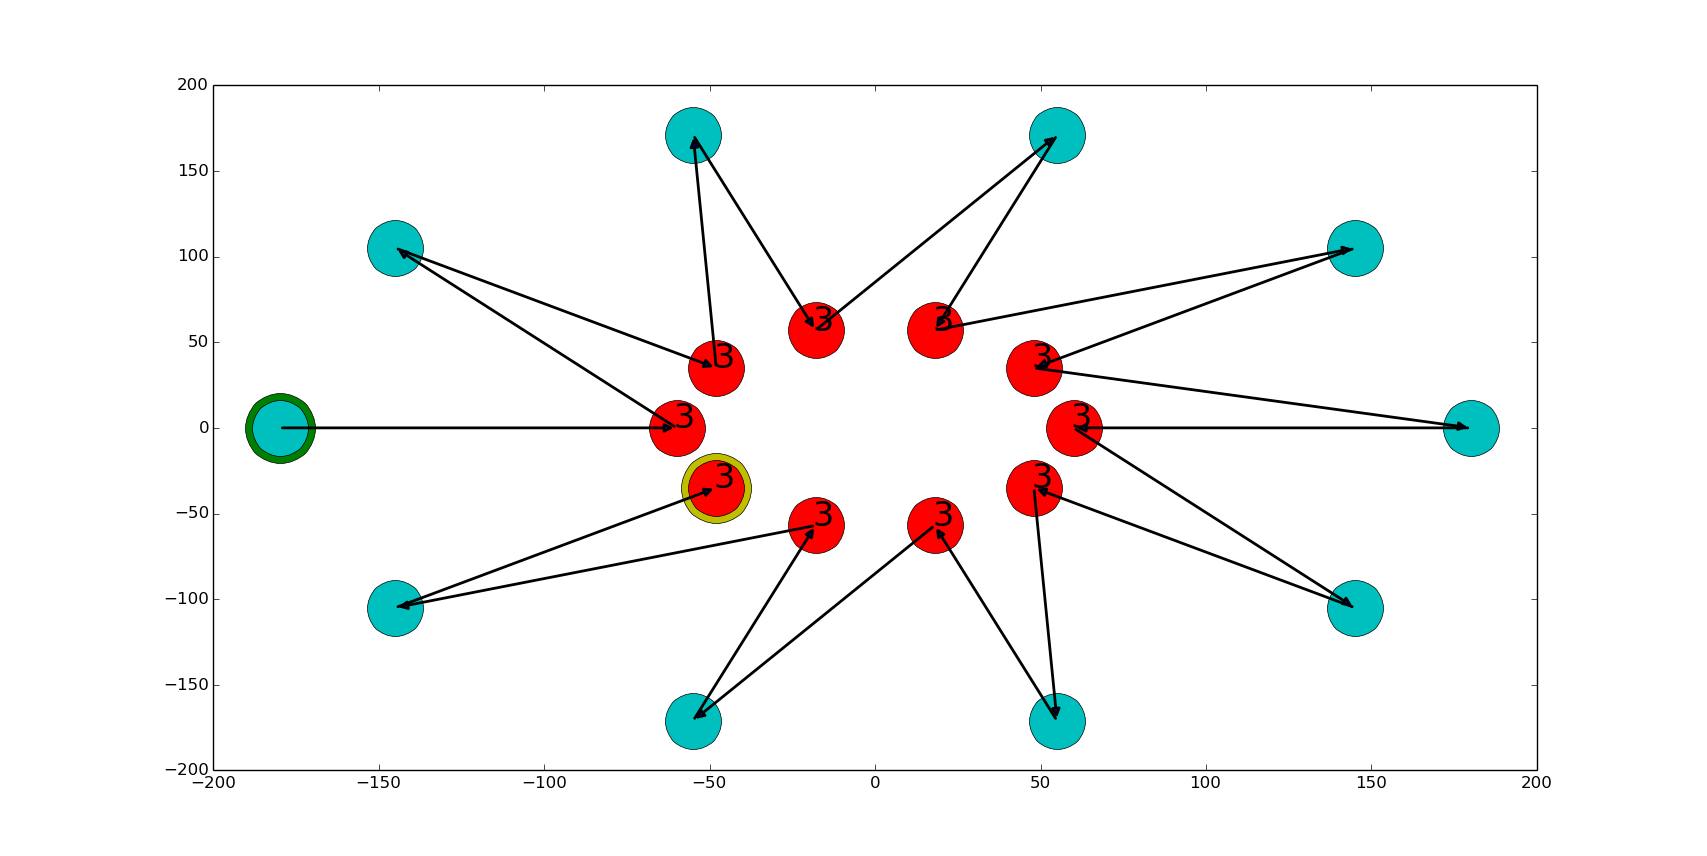
\includegraphics[scale=0.3]{./EJ4/fam7goloso.png}\\
 {            \textit{Soluci\'on Golosa}}
  \end{center}
  \vspace*{0.3cm}

\vspace*{0.3cm} \vspace*{0.3cm}
  \begin{center}
 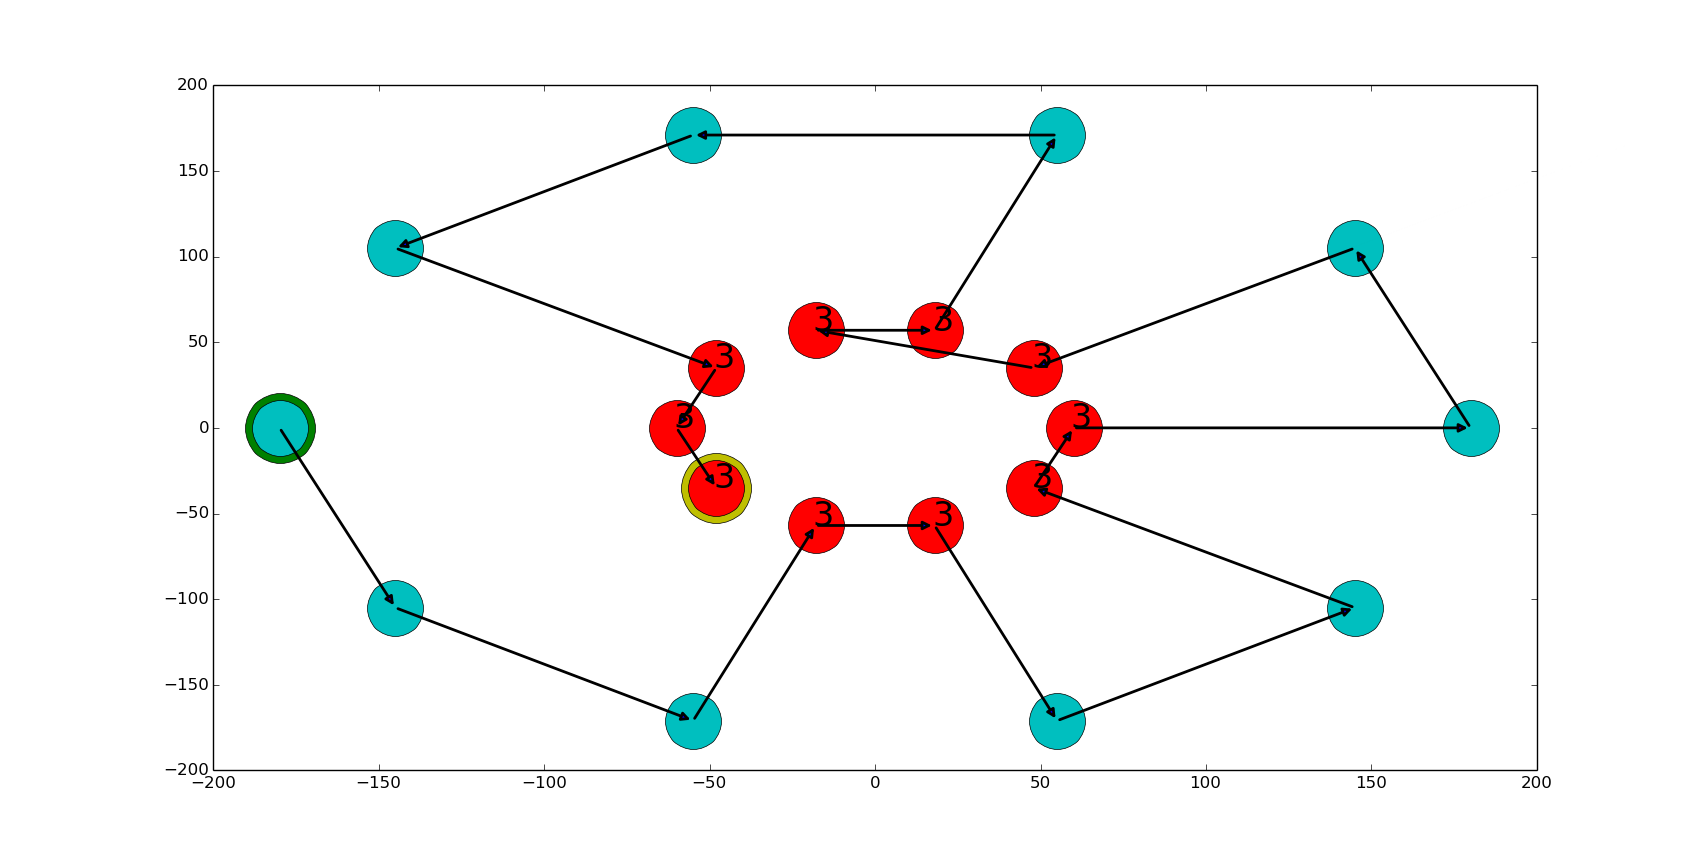
\includegraphics[scale=0.3]{./EJ4/fam72opt.png}\\
 {            \textit{Soluci\'on TABU 2-OPT}}
  \end{center}
  \vspace*{0.3cm}

\vspace*{0.3cm} \vspace*{0.3cm}
  \begin{center}
 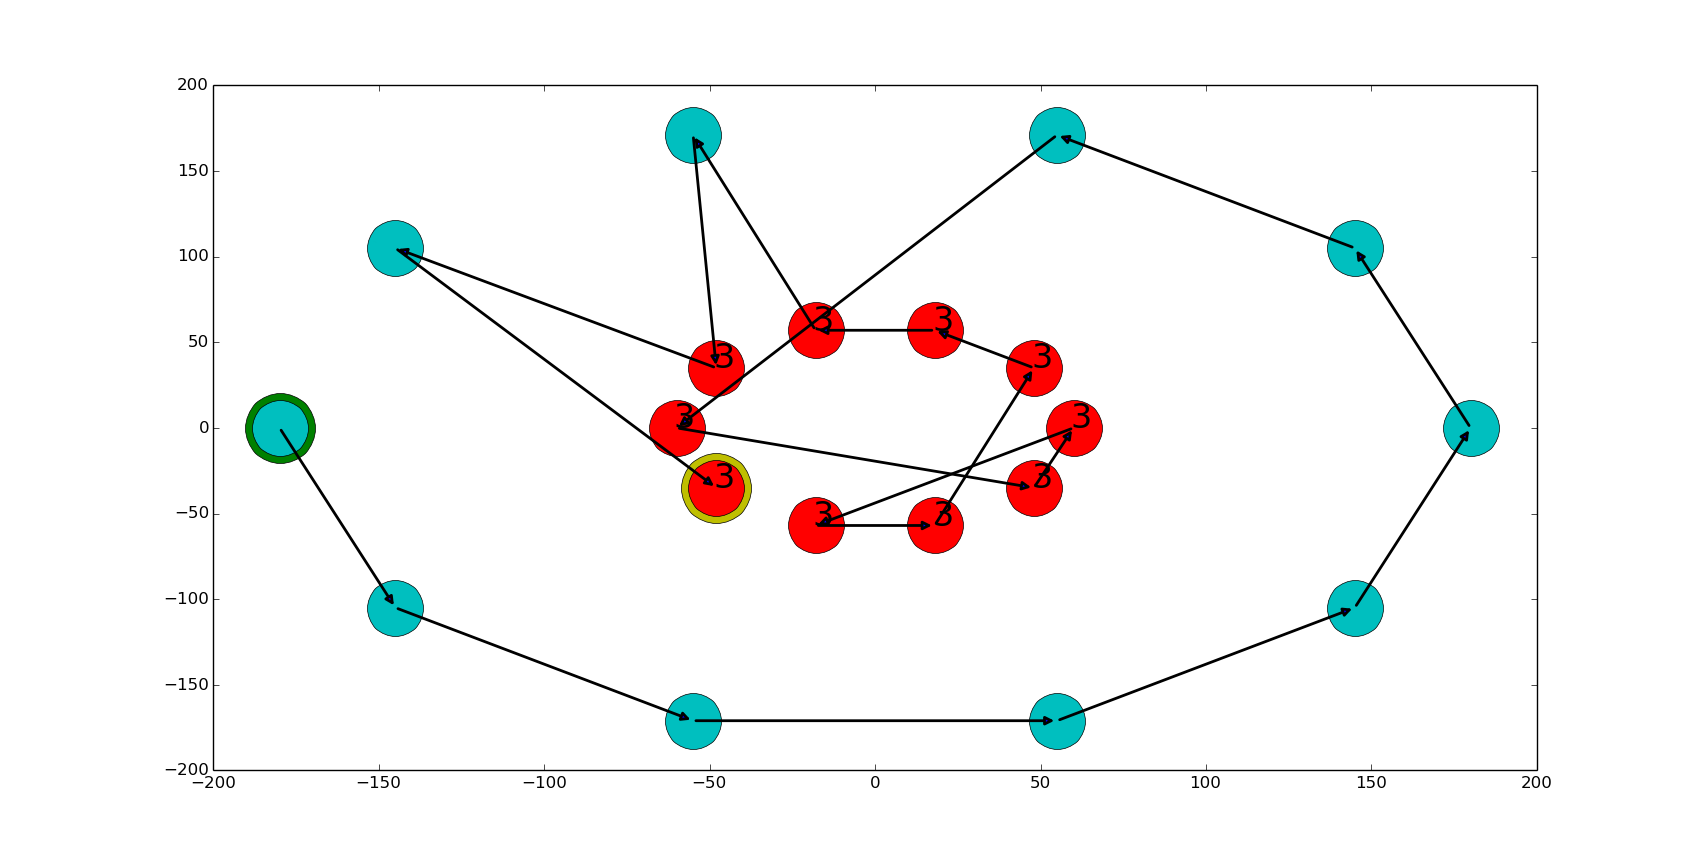
\includegraphics[scale=0.3]{./EJ4/fam73opt.png}\\
 {            \textit{Soluci\'on TABU 3-OPT}}
  \end{center}
  \vspace*{0.3cm}

Veamos como se comporta Tabu 2-OPT con respecto a la heuristica de busqueda local 2-OPT:

\vspace*{0.3cm} \vspace*{0.3cm}
  \begin{center}
 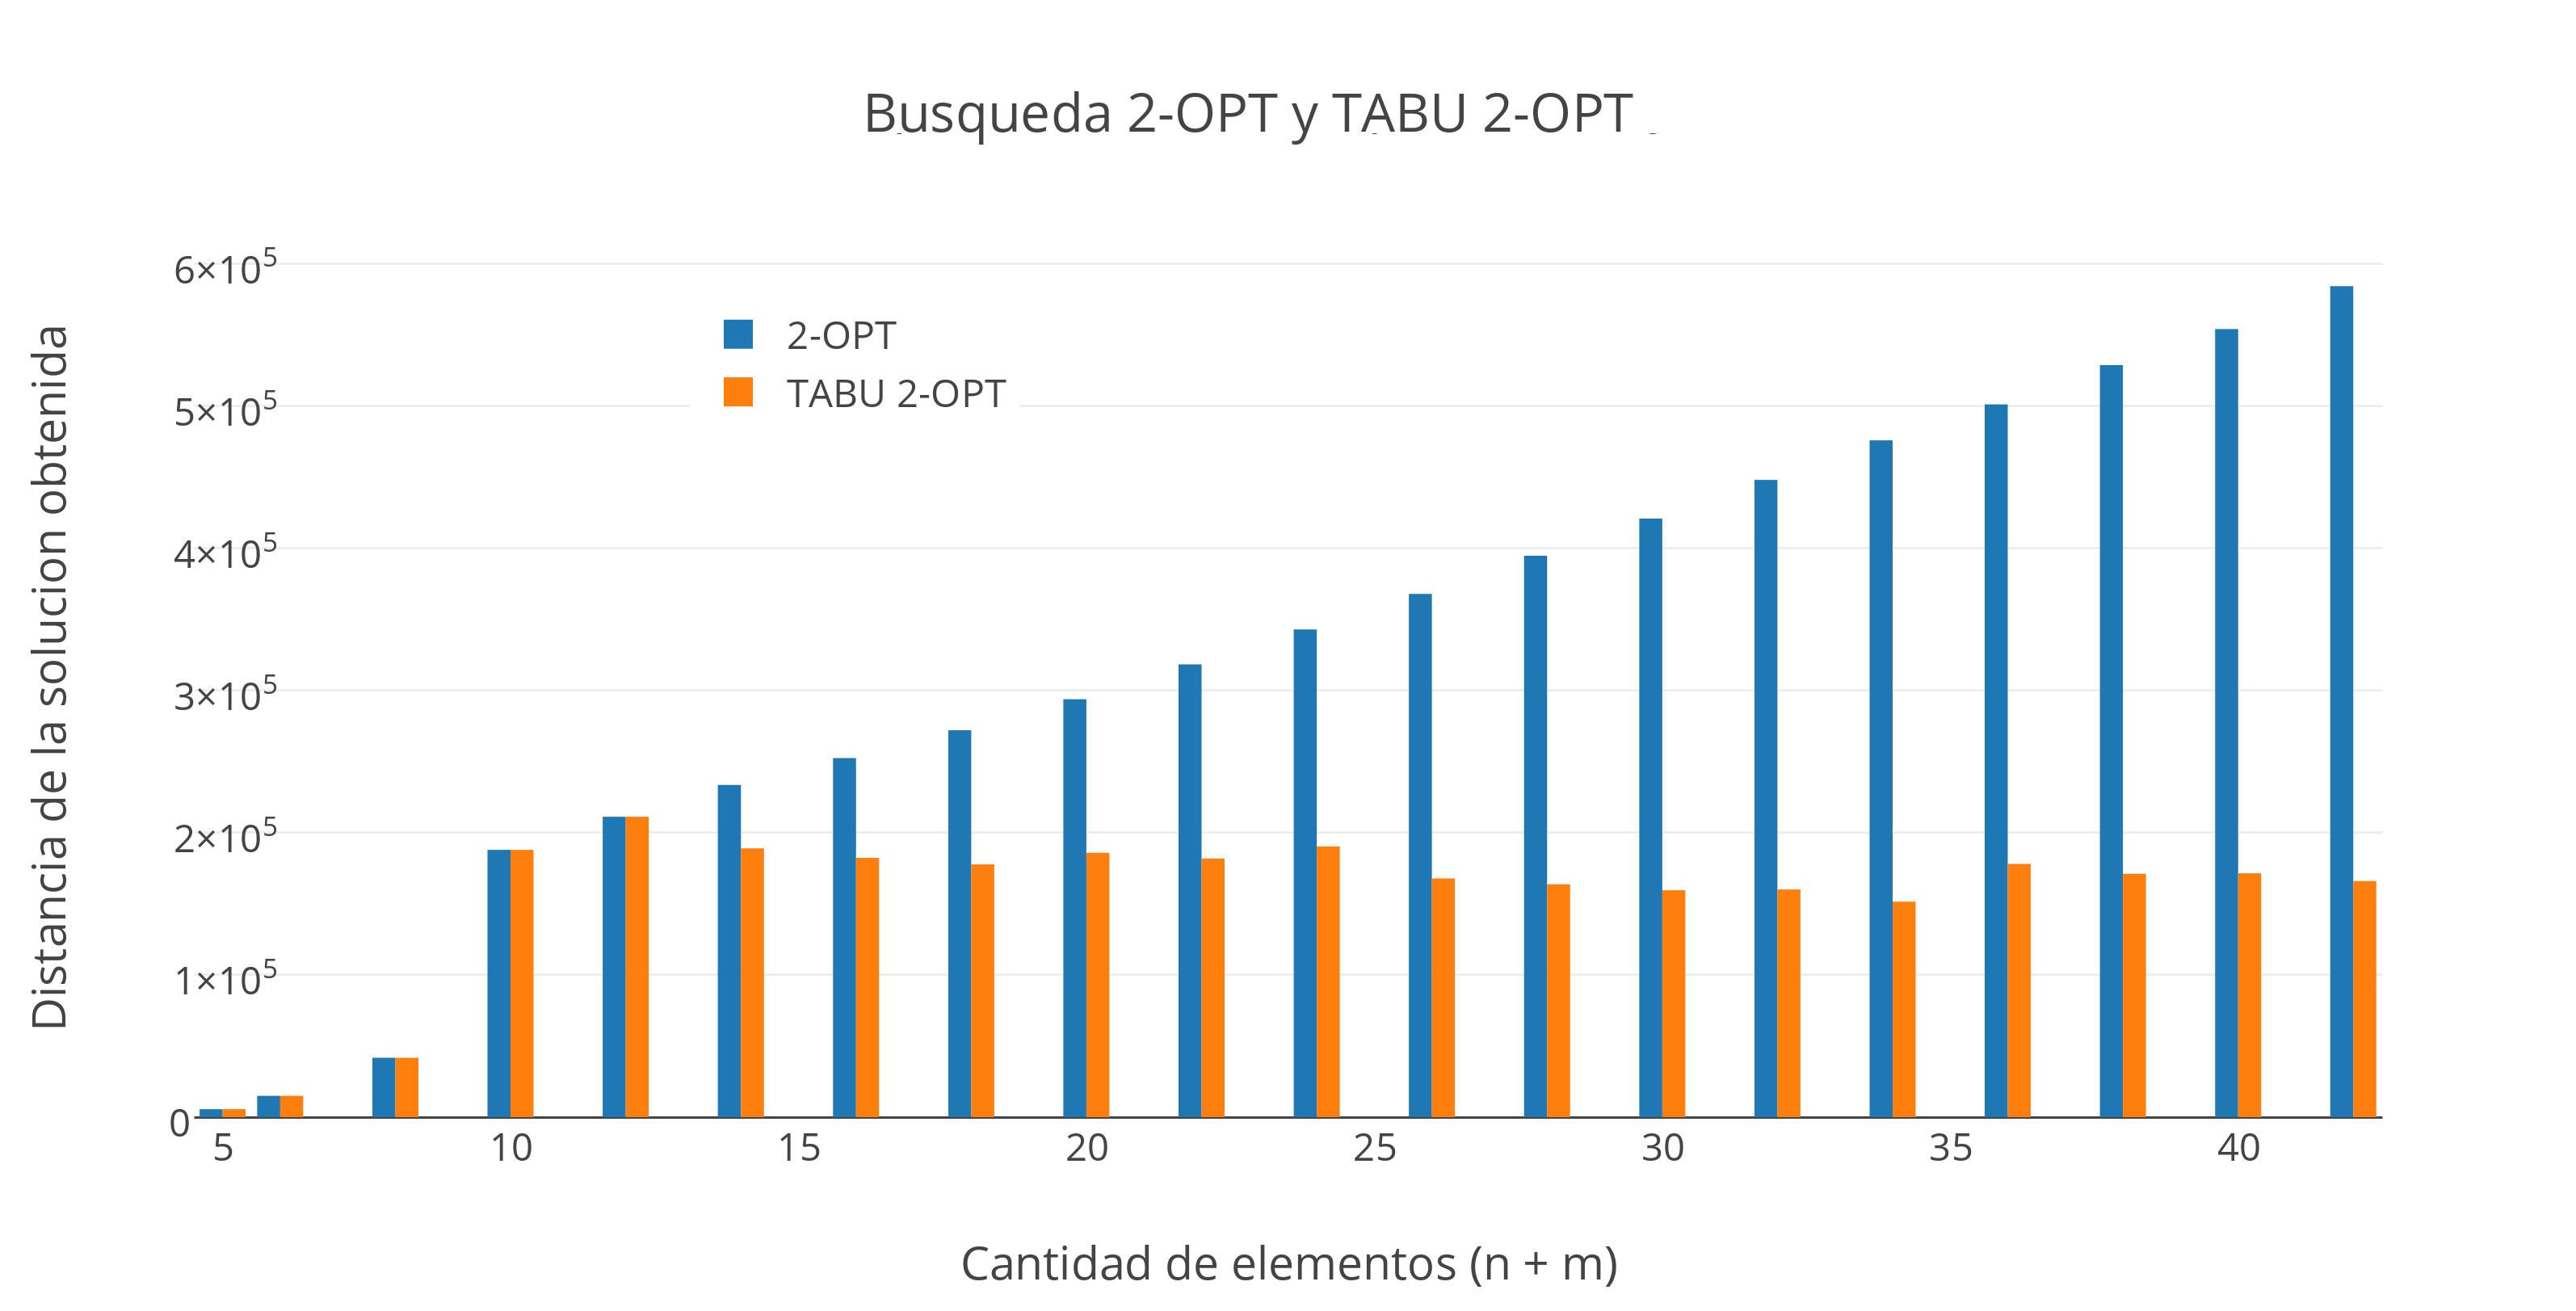
\includegraphics[scale=0.5]{./EJ4/comparativoanillos2opt.png}\\
 {            \textit{Gráfico \ 4.7 - 2-OPT vs Tabu 2-OPT sobre Familia 7}}
  \end{center}
  \vspace*{0.3cm}

\vspace*{0.3cm} \vspace*{0.3cm}
  \begin{center}
 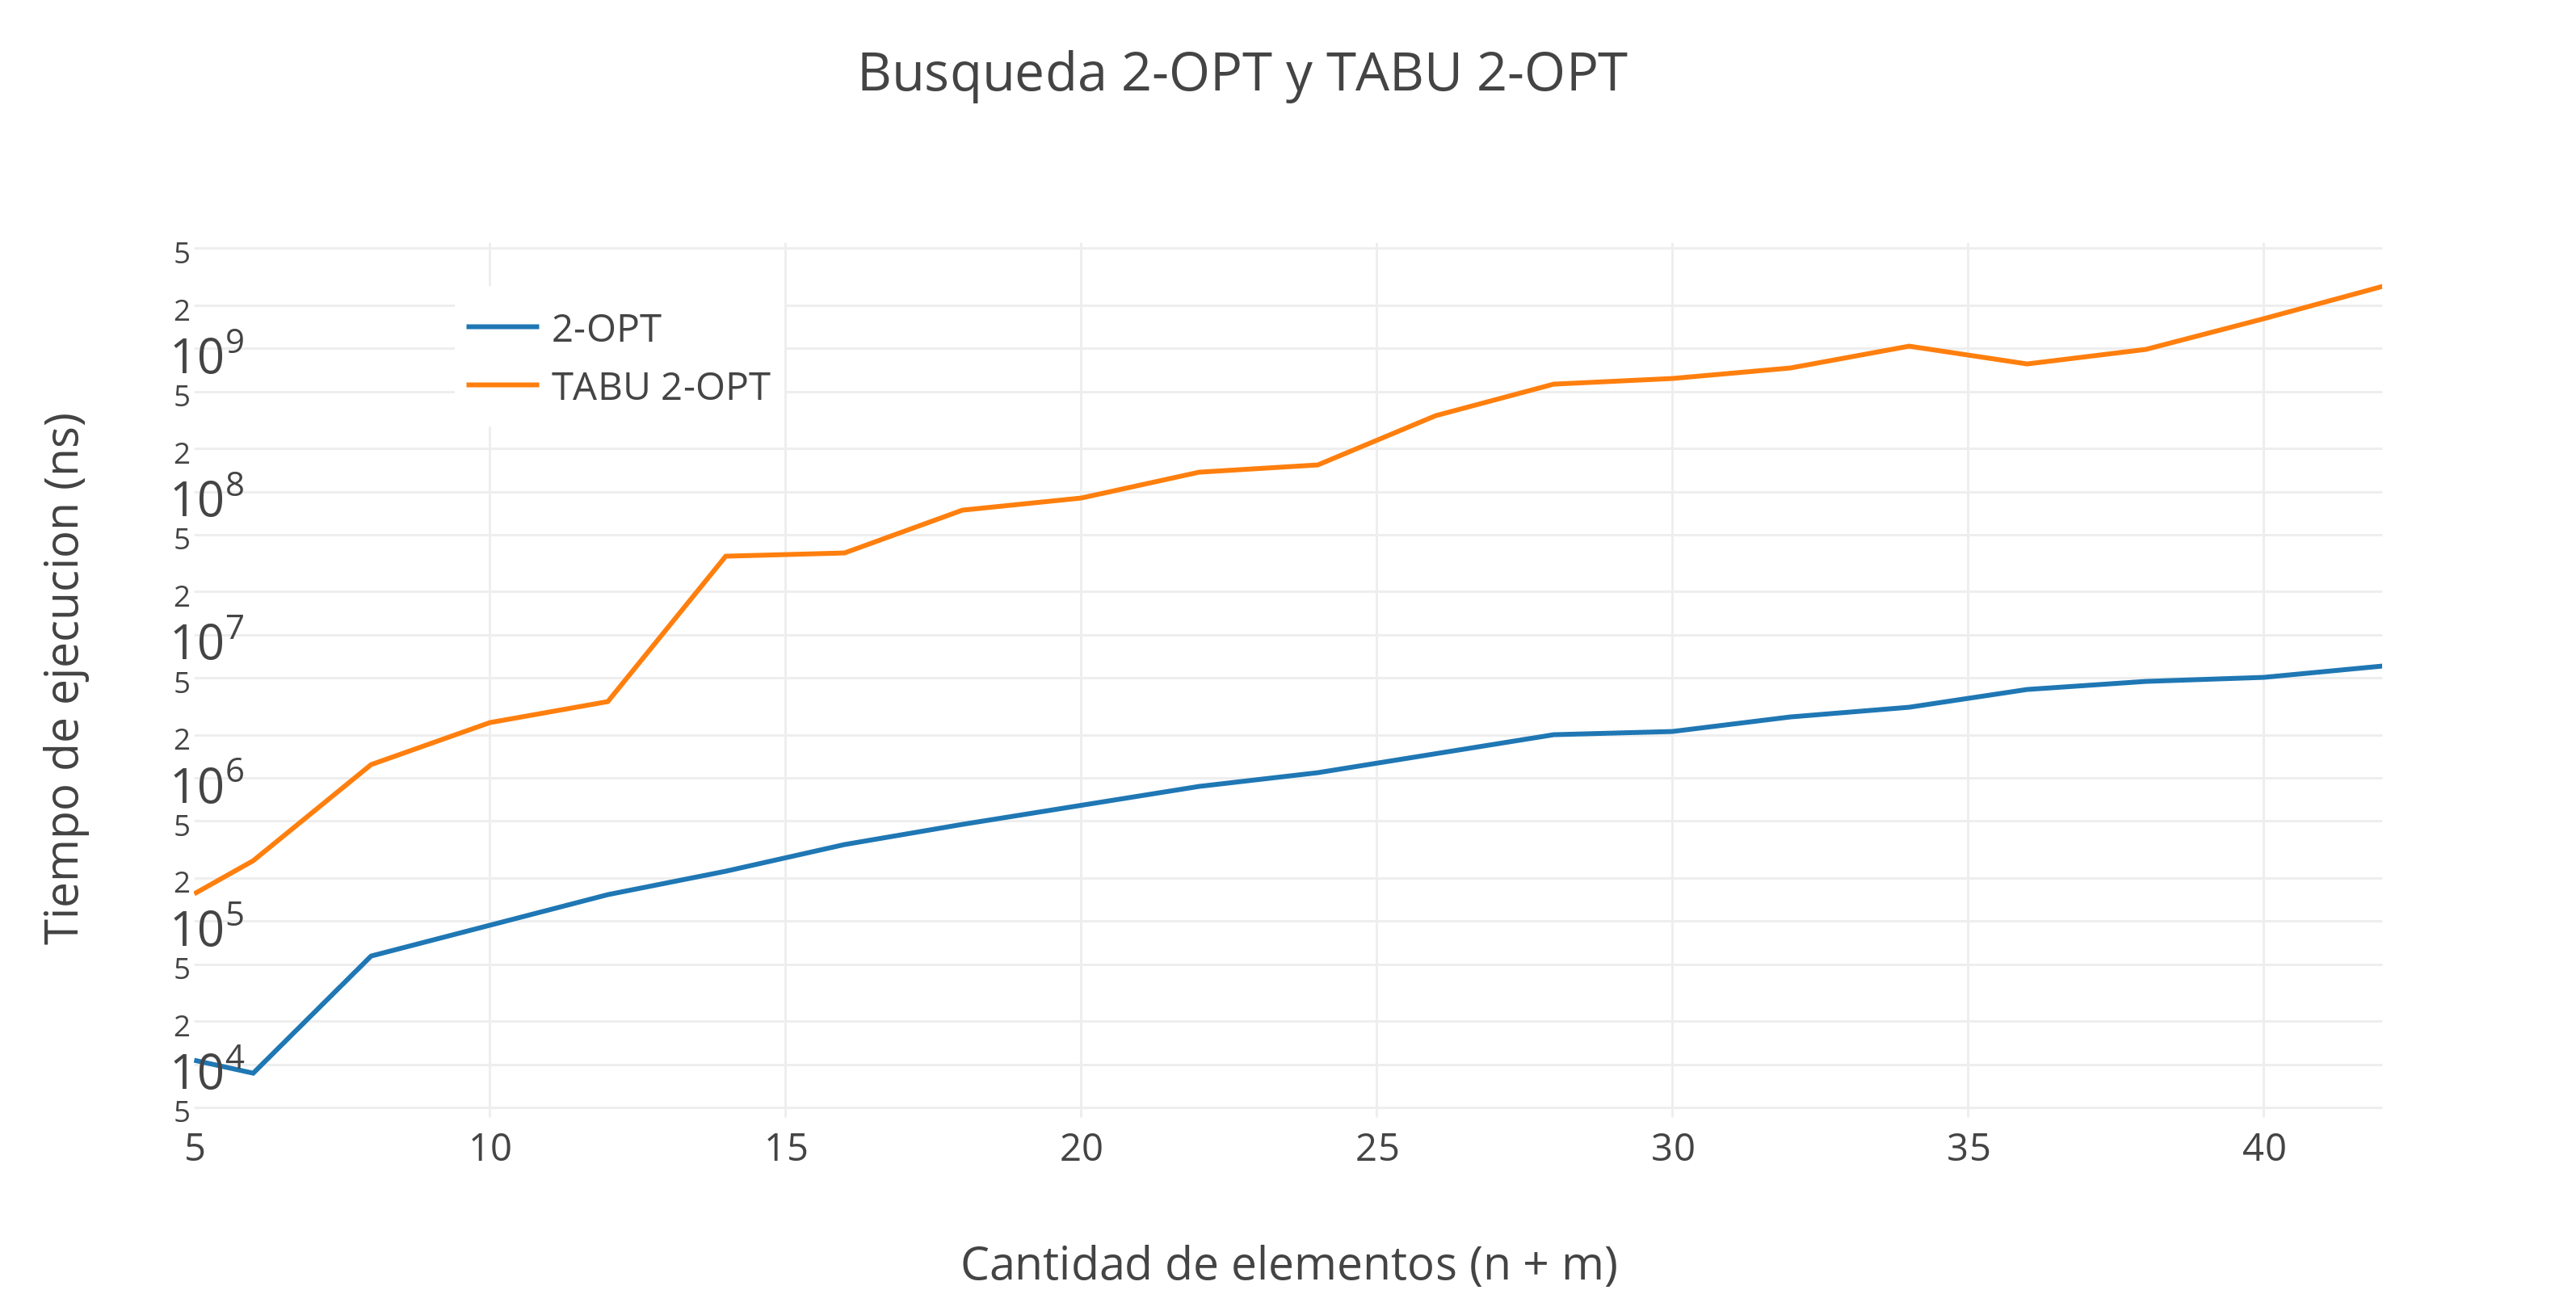
\includegraphics[scale=0.5]{./EJ4/medicionanillos2opt.png}\\
 {            \textit{Gráfico \ 4.8 - 2-OPT vs Tabu 2-OPT sobre Familia 7}}
  \end{center}
  \vspace*{0.3cm}

Luego, para 3-OPT:

\vspace*{0.3cm} \vspace*{0.3cm}
  \begin{center}
 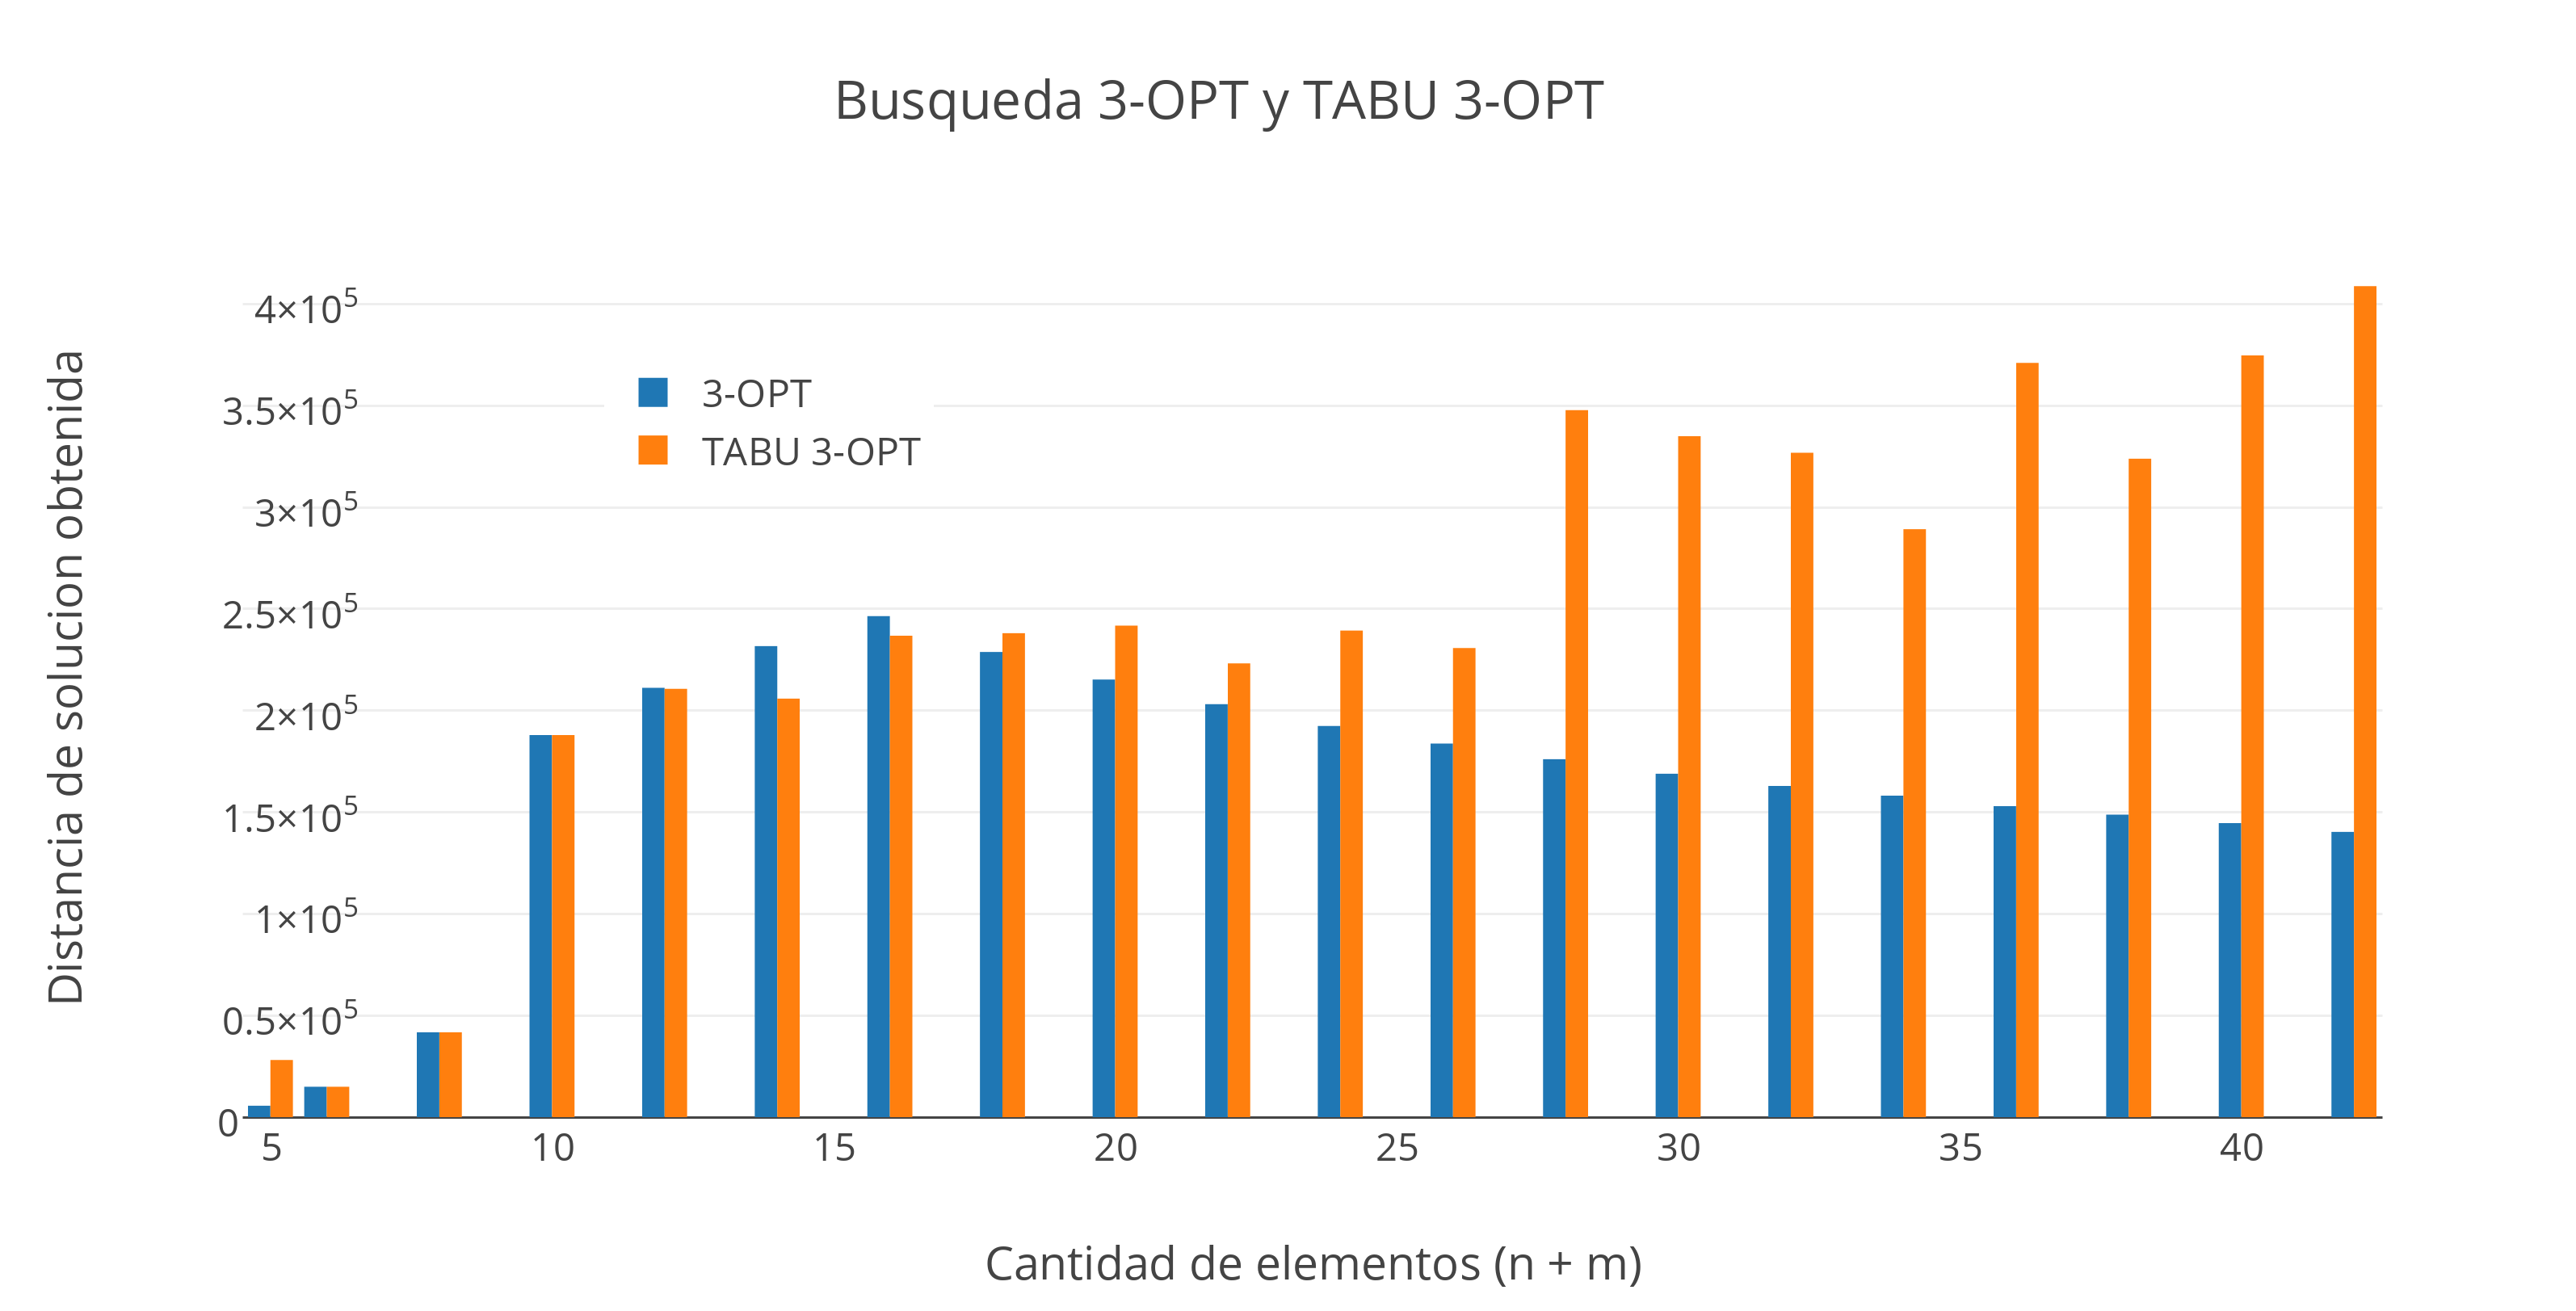
\includegraphics[scale=0.5]{./EJ4/comparativoanillos3opt.png}\\
 {            \textit{Gráfico \ 4.9 - 3-OPT vs Tabu 3-OPT sobre Familia 7}}
  \end{center}
  \vspace*{0.3cm}

\vspace*{0.3cm} \vspace*{0.3cm}
  \begin{center}
 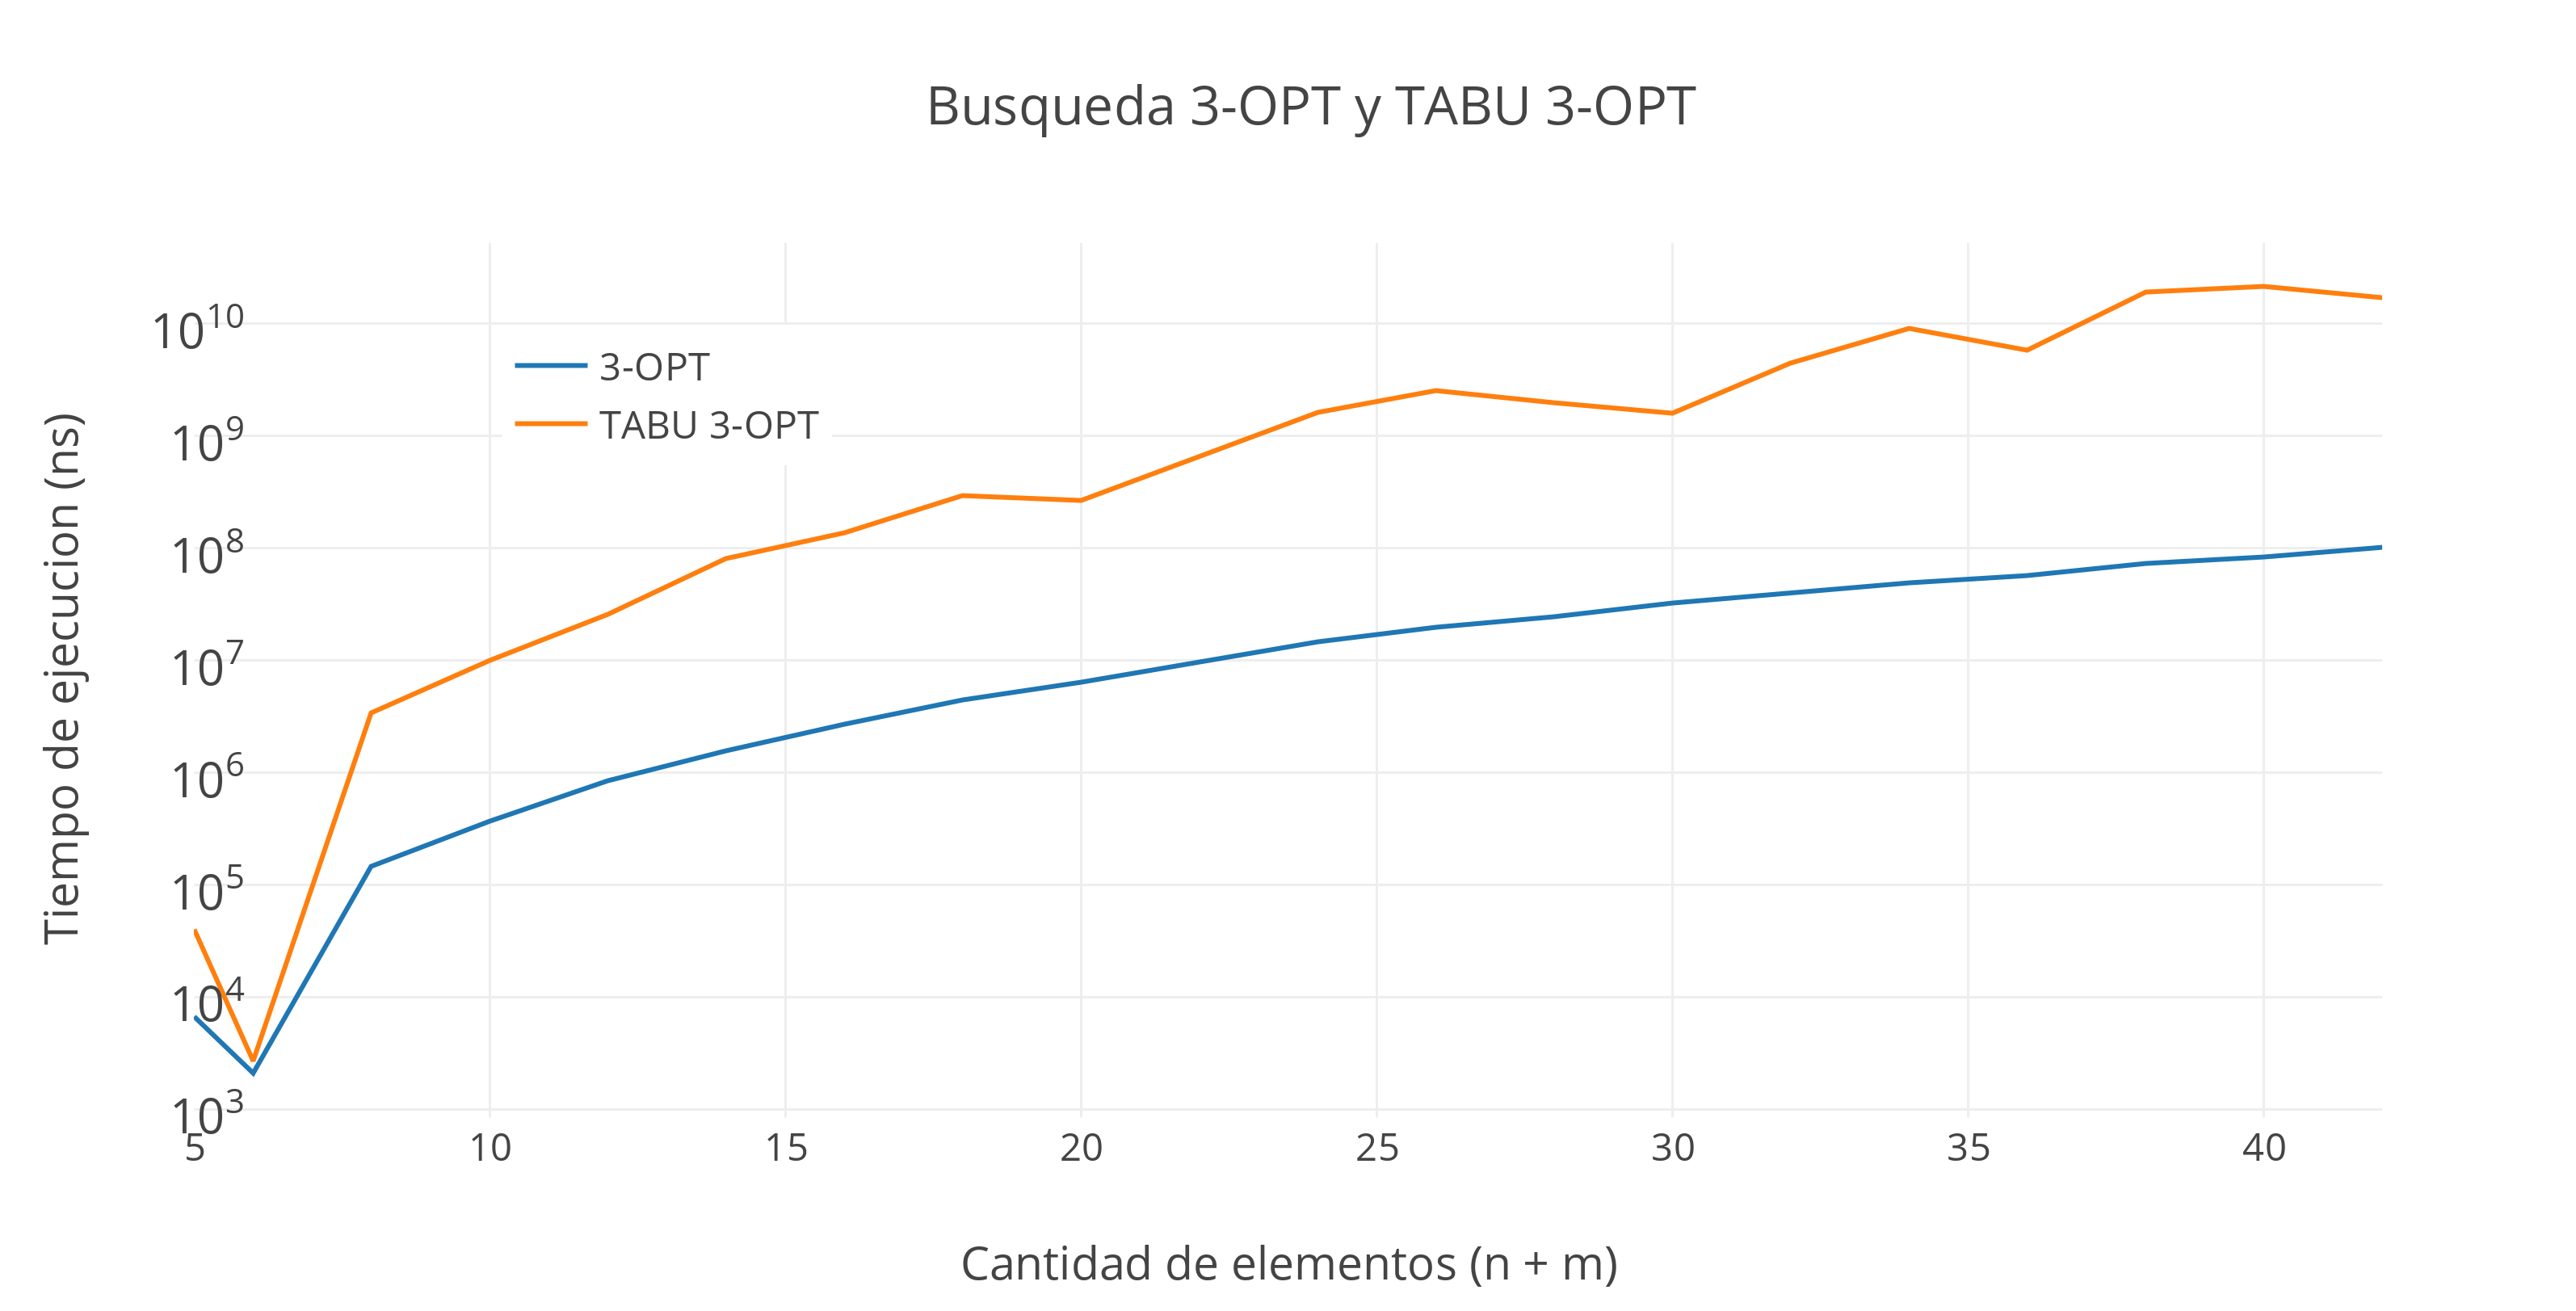
\includegraphics[scale=0.5]{./EJ4/medicionanillos3opt.png}\\
 {            \textit{Gráfico \ 4.10 - 3-OPT vs Tabu 3-OPT sobre Familia 7}}
  \end{center}
  \vspace*{0.3cm}
  
Habiendo chequeado dichos experimentos, pudimos observar que para esta familia sucede algo muy similar que en la n\'umero 6 donde al utilizar Tabu 2-OPT la solucion obtenida es considerablemente mejor que la obtenida por 2-OPT. 
Y al igual que en la familia anterior, el otro Tabu, presenta un peor desempeño. Ya que las soluciones obtenidas son hasta 3 veces peores que las obtenidas por la busqueda local 3-OPT.
 
Comparando las soluciones de cada version de tabú search podemos observar lo siguiente: 
  
\vspace*{0.3cm} \vspace*{0.3cm}
  \begin{center}
 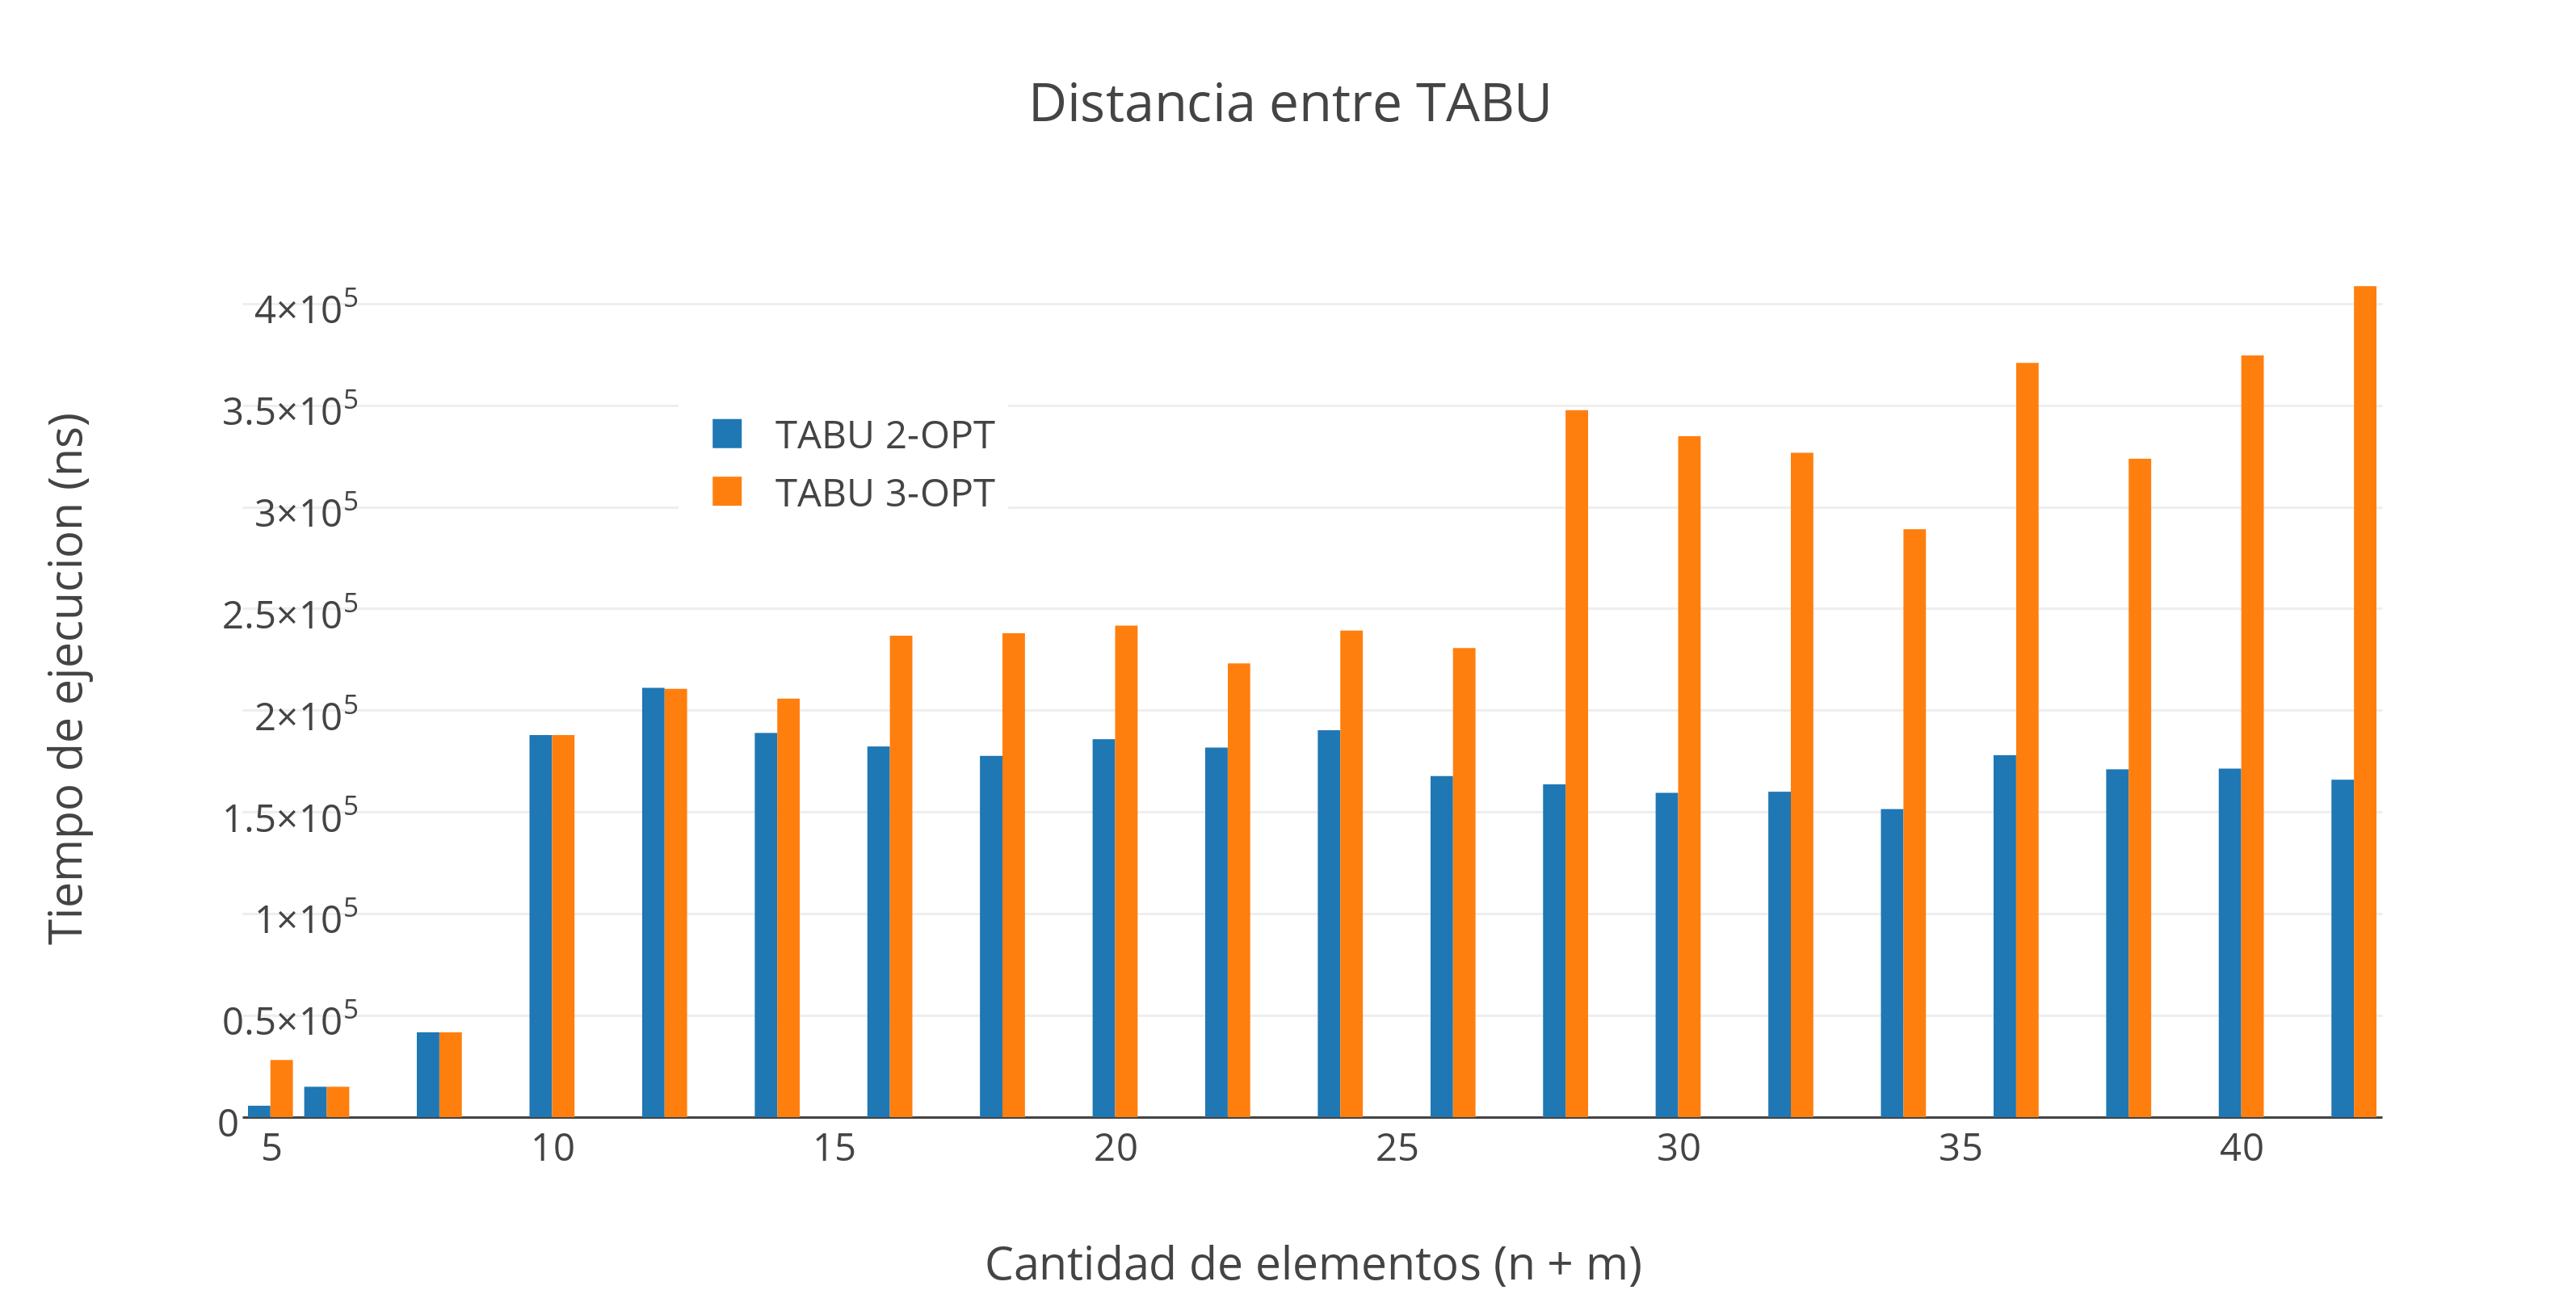
\includegraphics[scale=0.5]{./EJ4/comparativoanillos1.png}\\
 {            \textit{Gráfico \ 4.11 - Tabu 2-OPT vs Tabu 3-OPT sobre Familia 7}}
  \end{center}
  \vspace*{0.3cm}

\vspace*{0.3cm} \vspace*{0.3cm}
  \begin{center}
 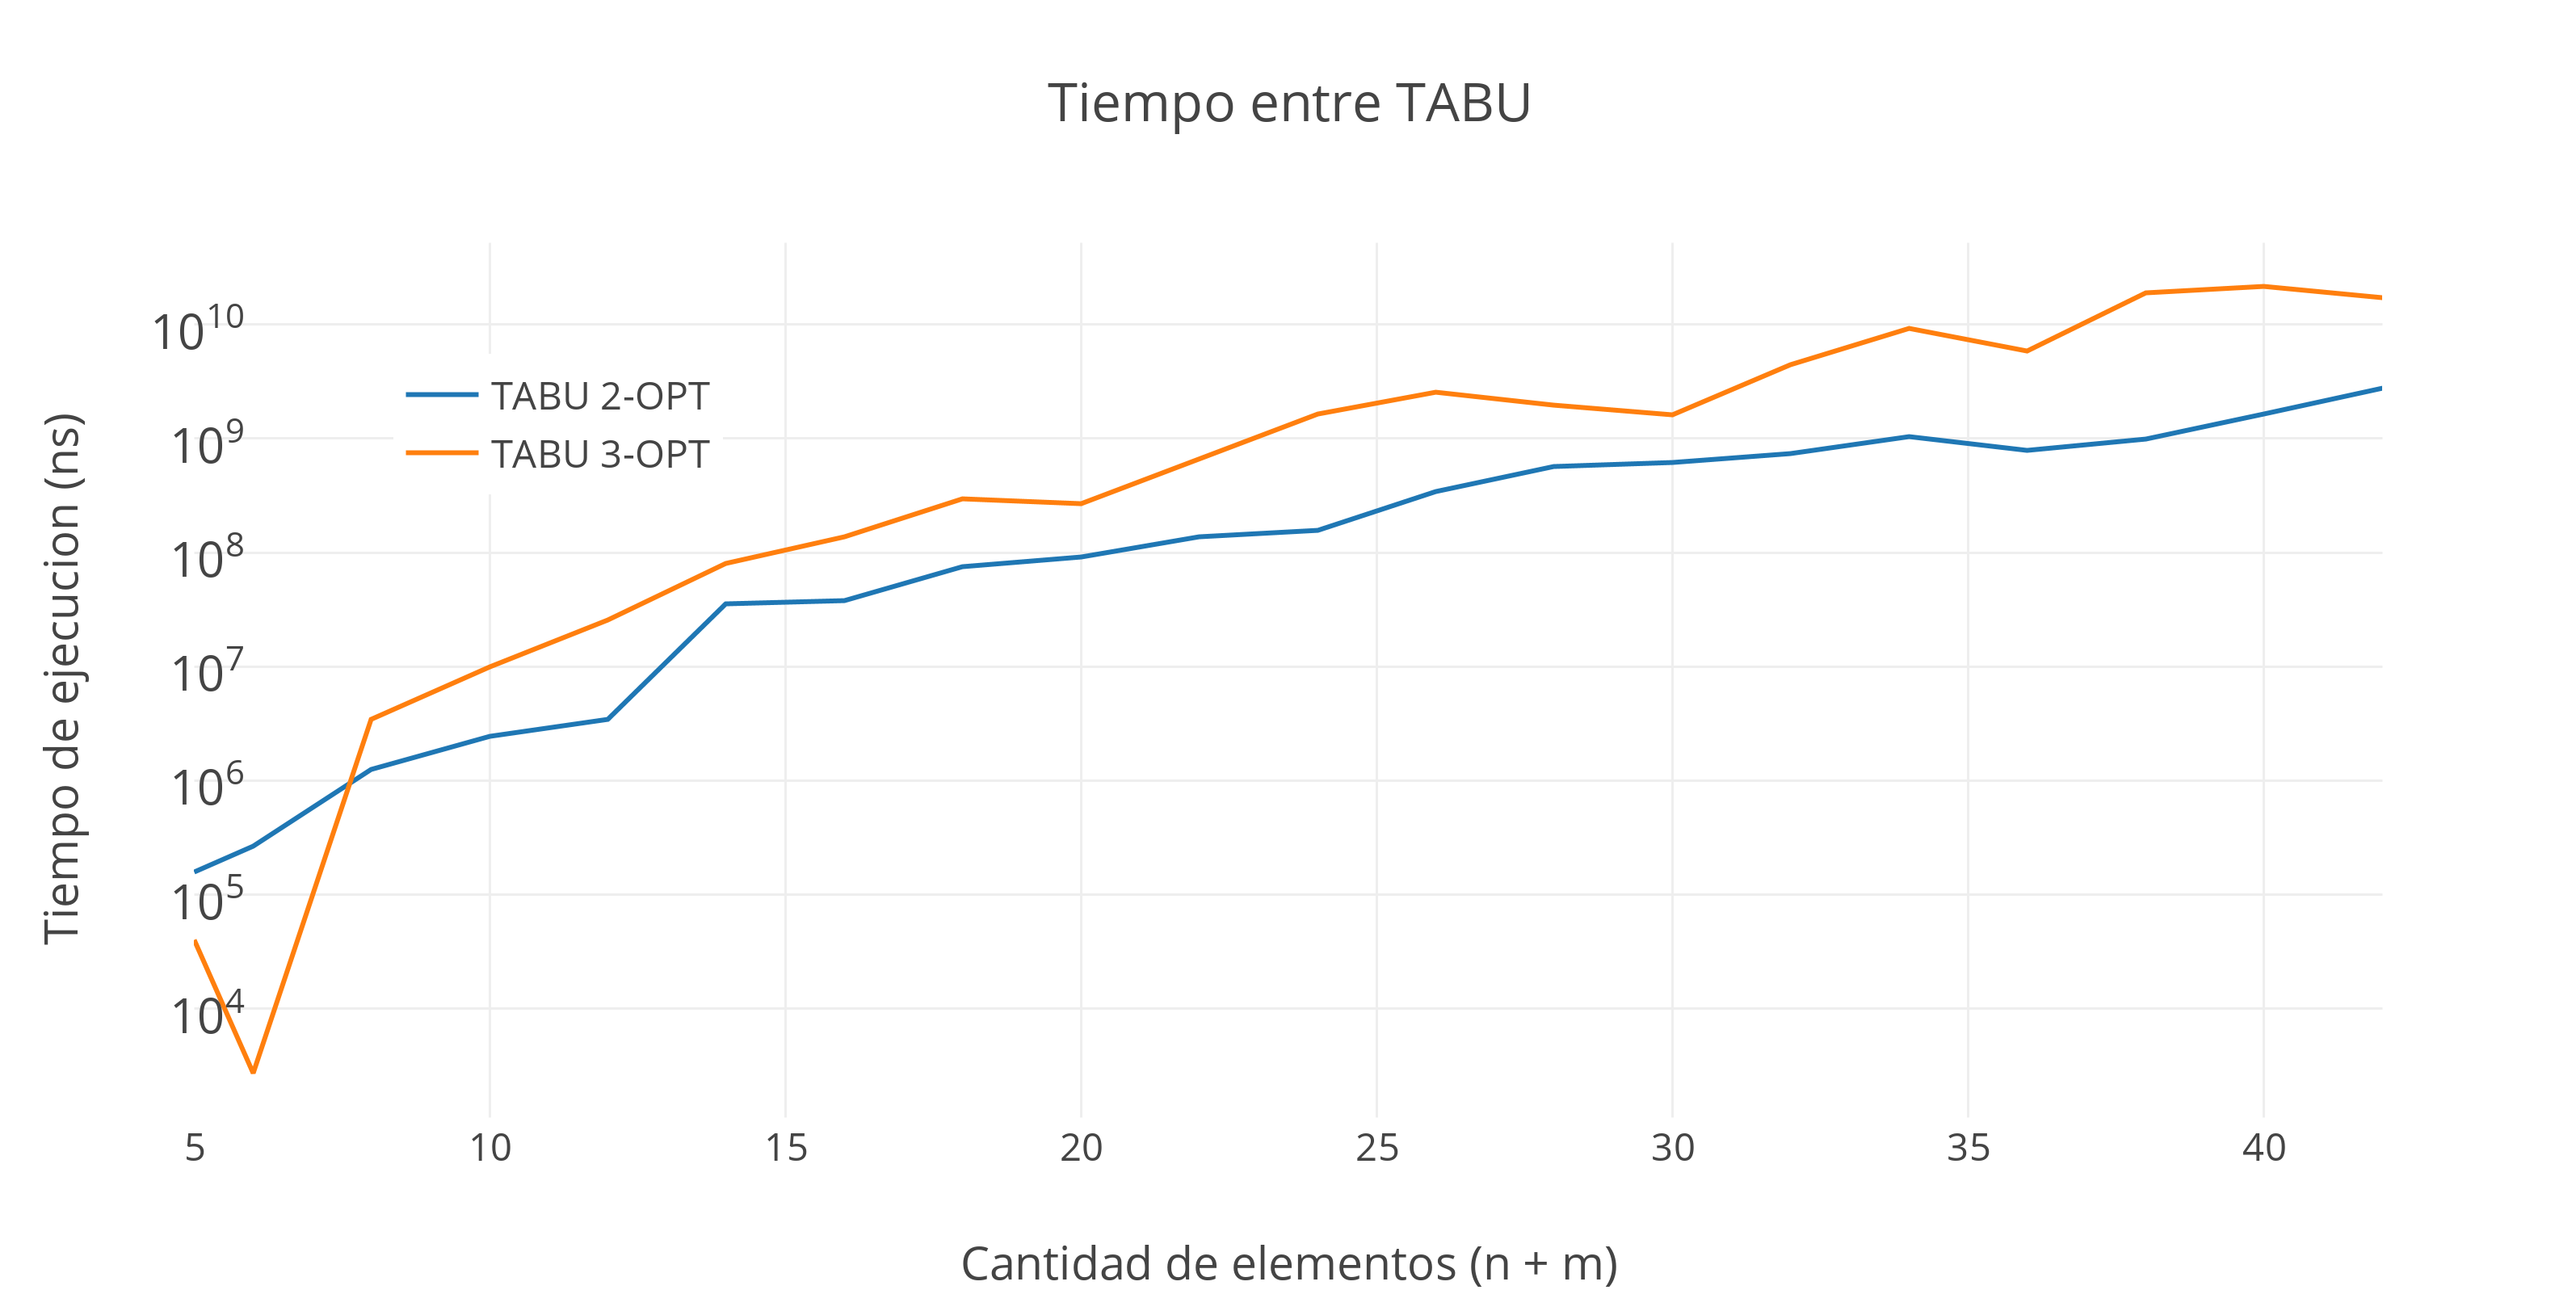
\includegraphics[scale=0.5]{./EJ4/comparativoanillos.png}\\
 {            \textit{Gráfico \ 4.12 - Tabu 2-OPT vs Tabu 3-OPT sobre Familia 7}}
  \end{center}
  \vspace*{0.3cm}
  
Dando por finalizada la comparaciones entre Tabu, como mencionamos, a la hora de trabajar con alguna de las dos para esta familia, la mejor en relaci\'on tiempo-calidad de soluci\'on ser\'a Tabu 2-OPT.

\subsubsection*{Familia 8}

Esta familia, como se denomino, es random, la misma fue implementada de la forma en la que siempre se obtenga soluci\'on, o sea, siempre exista la cantidad necesaria de Pokeparadas para vencer a todos los gimnasios y la capacidad de la mochila sea acorde a la cantidad de pociones necesarias para poder vencer al gimnasio mas poderoso.

Por la particularidad de la misma, las soluciones y el tiempo insumido para obtener las mismas suele ser variable. Se intentar\'a por medio de las meta-heuristicas trabajadas mejorar en caso de ser posible la soluci\'on obtenida por el goloso.

Un ejemplo de como es cambia el camino del goloso por las meta heur\'isticas es el siguiente:\\

\vspace*{0.3cm} \vspace*{0.3cm}
  \begin{center}
 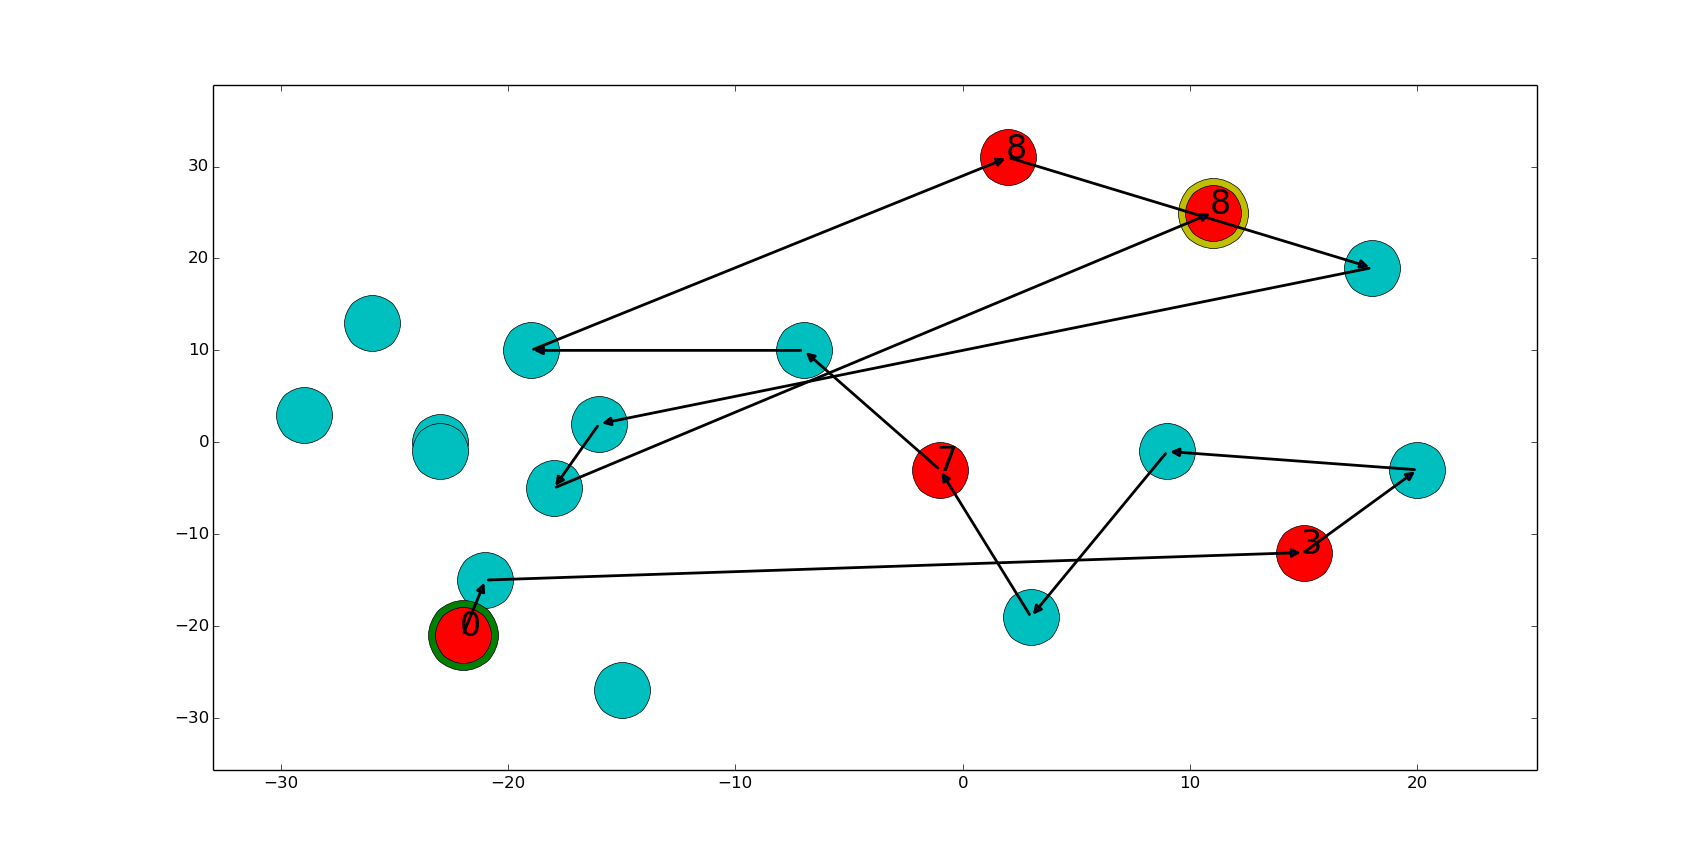
\includegraphics[scale=0.3]{./EJ4/fam8goloso.png}\\
 {            \textit{Soluci\'on Golosa}}
  \end{center}
  \vspace*{0.3cm}

\vspace*{0.3cm} \vspace*{0.3cm}
  \begin{center}
 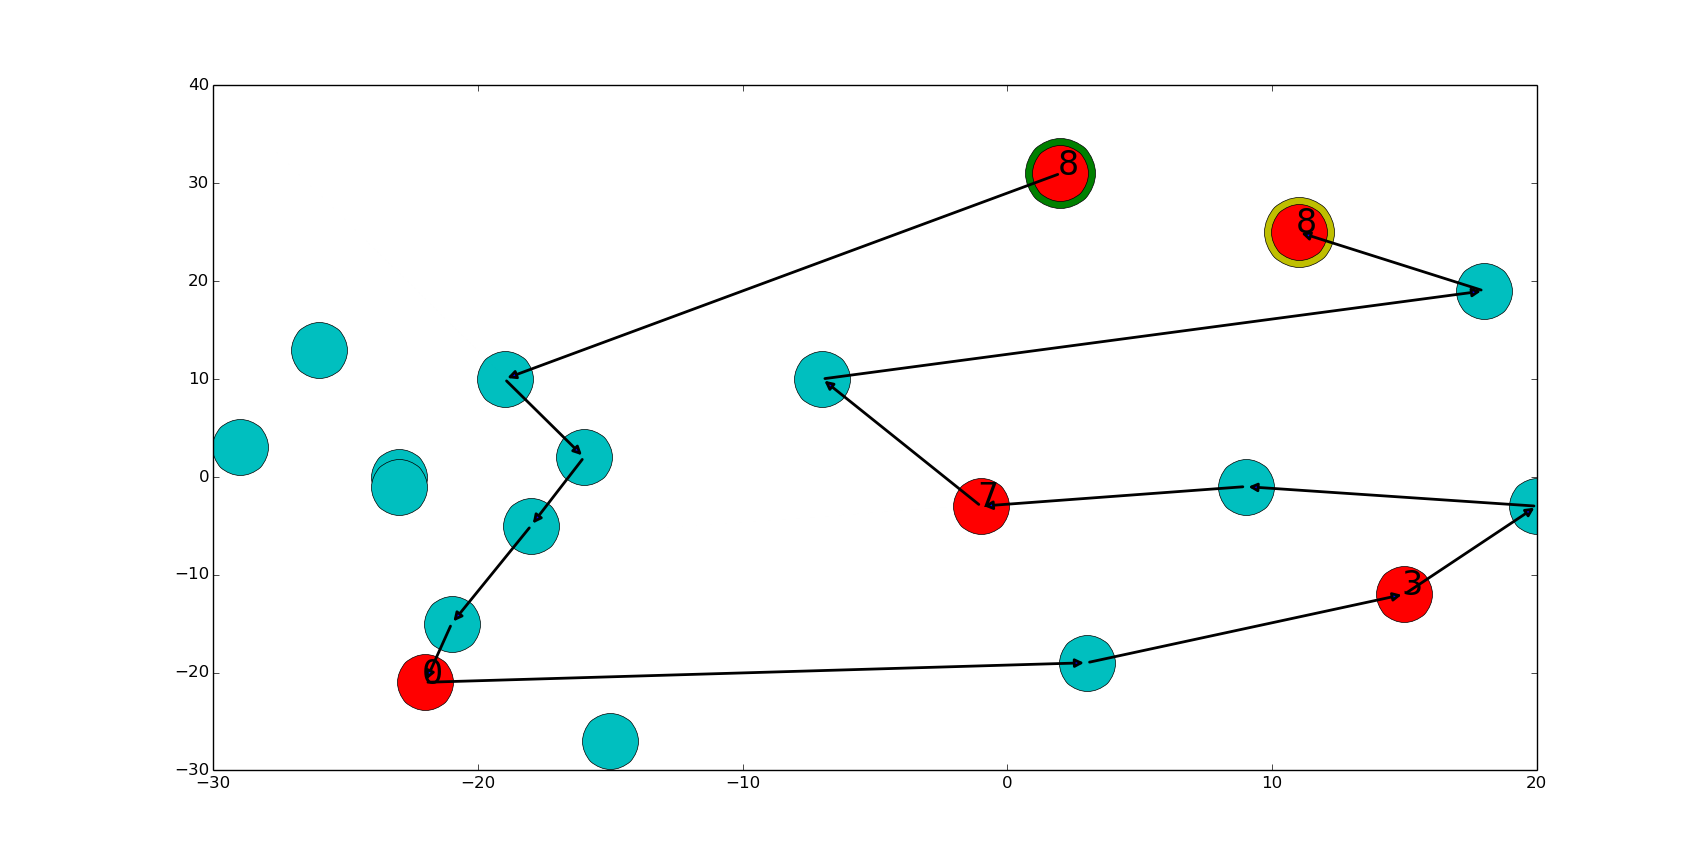
\includegraphics[scale=0.3]{./EJ4/fam82opt.png}\\
 {            \textit{Soluci\'on TABU 2-OPT}}
  \end{center}
  \vspace*{0.3cm}

\vspace*{0.3cm} \vspace*{0.3cm}
  \begin{center}
 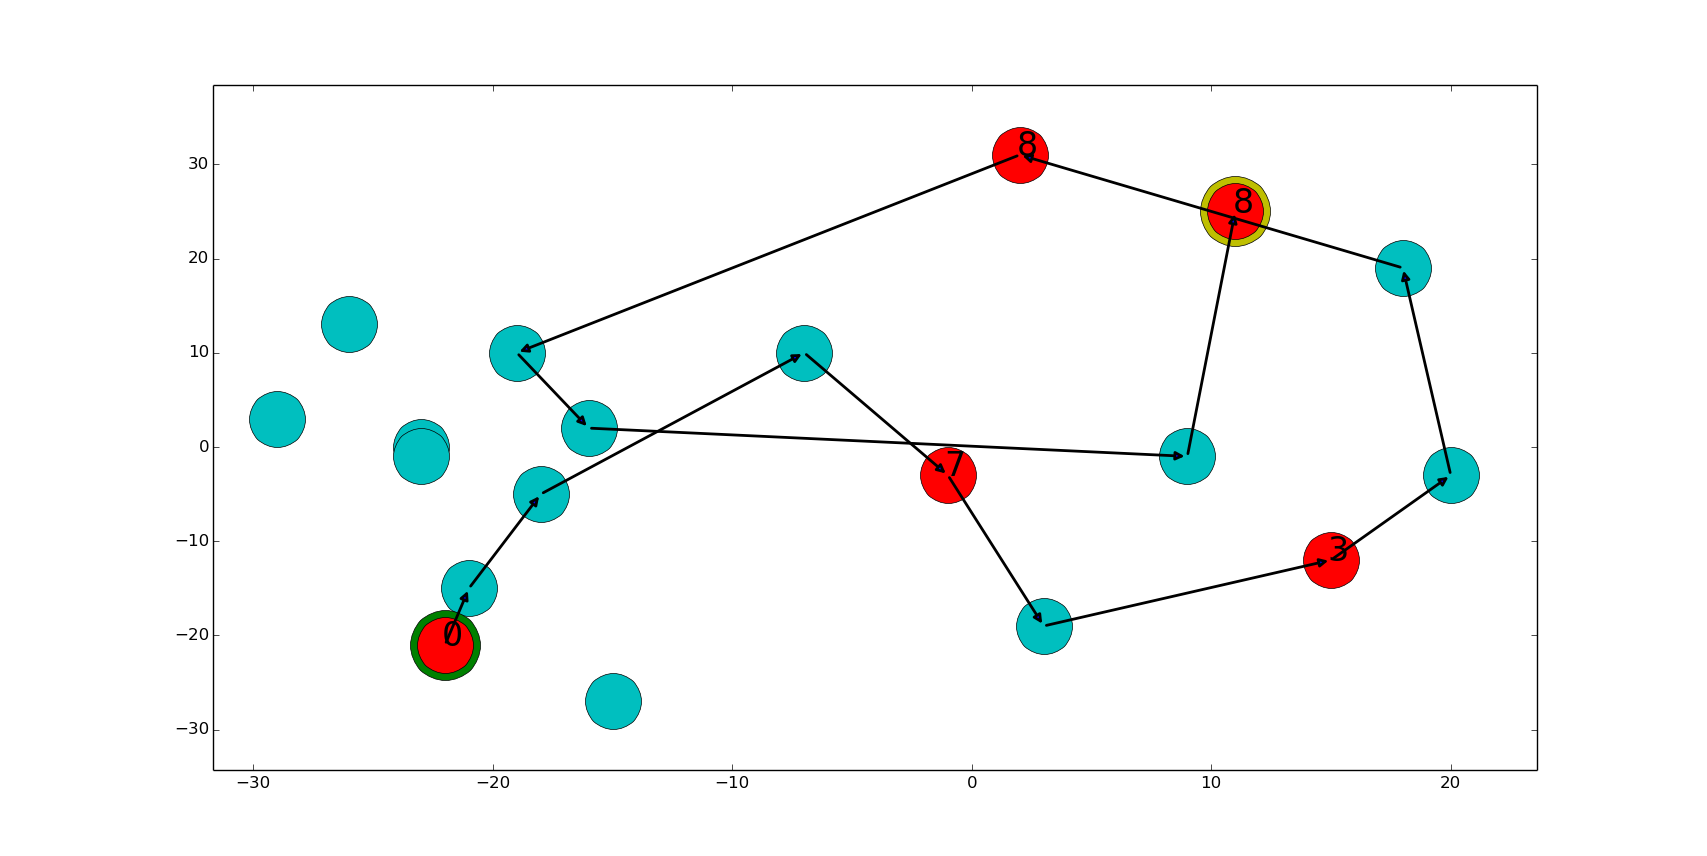
\includegraphics[scale=0.3]{./EJ4/fam83opt.png}\\
 {            \textit{Soluci\'on TABU 3-OPT}}
  \end{center}
  \vspace*{0.3cm}

Veamos como se comporta Tabu 2-OPT con respecto a la heur\'istica de b\'usqueda local 2-OPT:

\vspace*{0.3cm} \vspace*{0.3cm}
  \begin{center}
 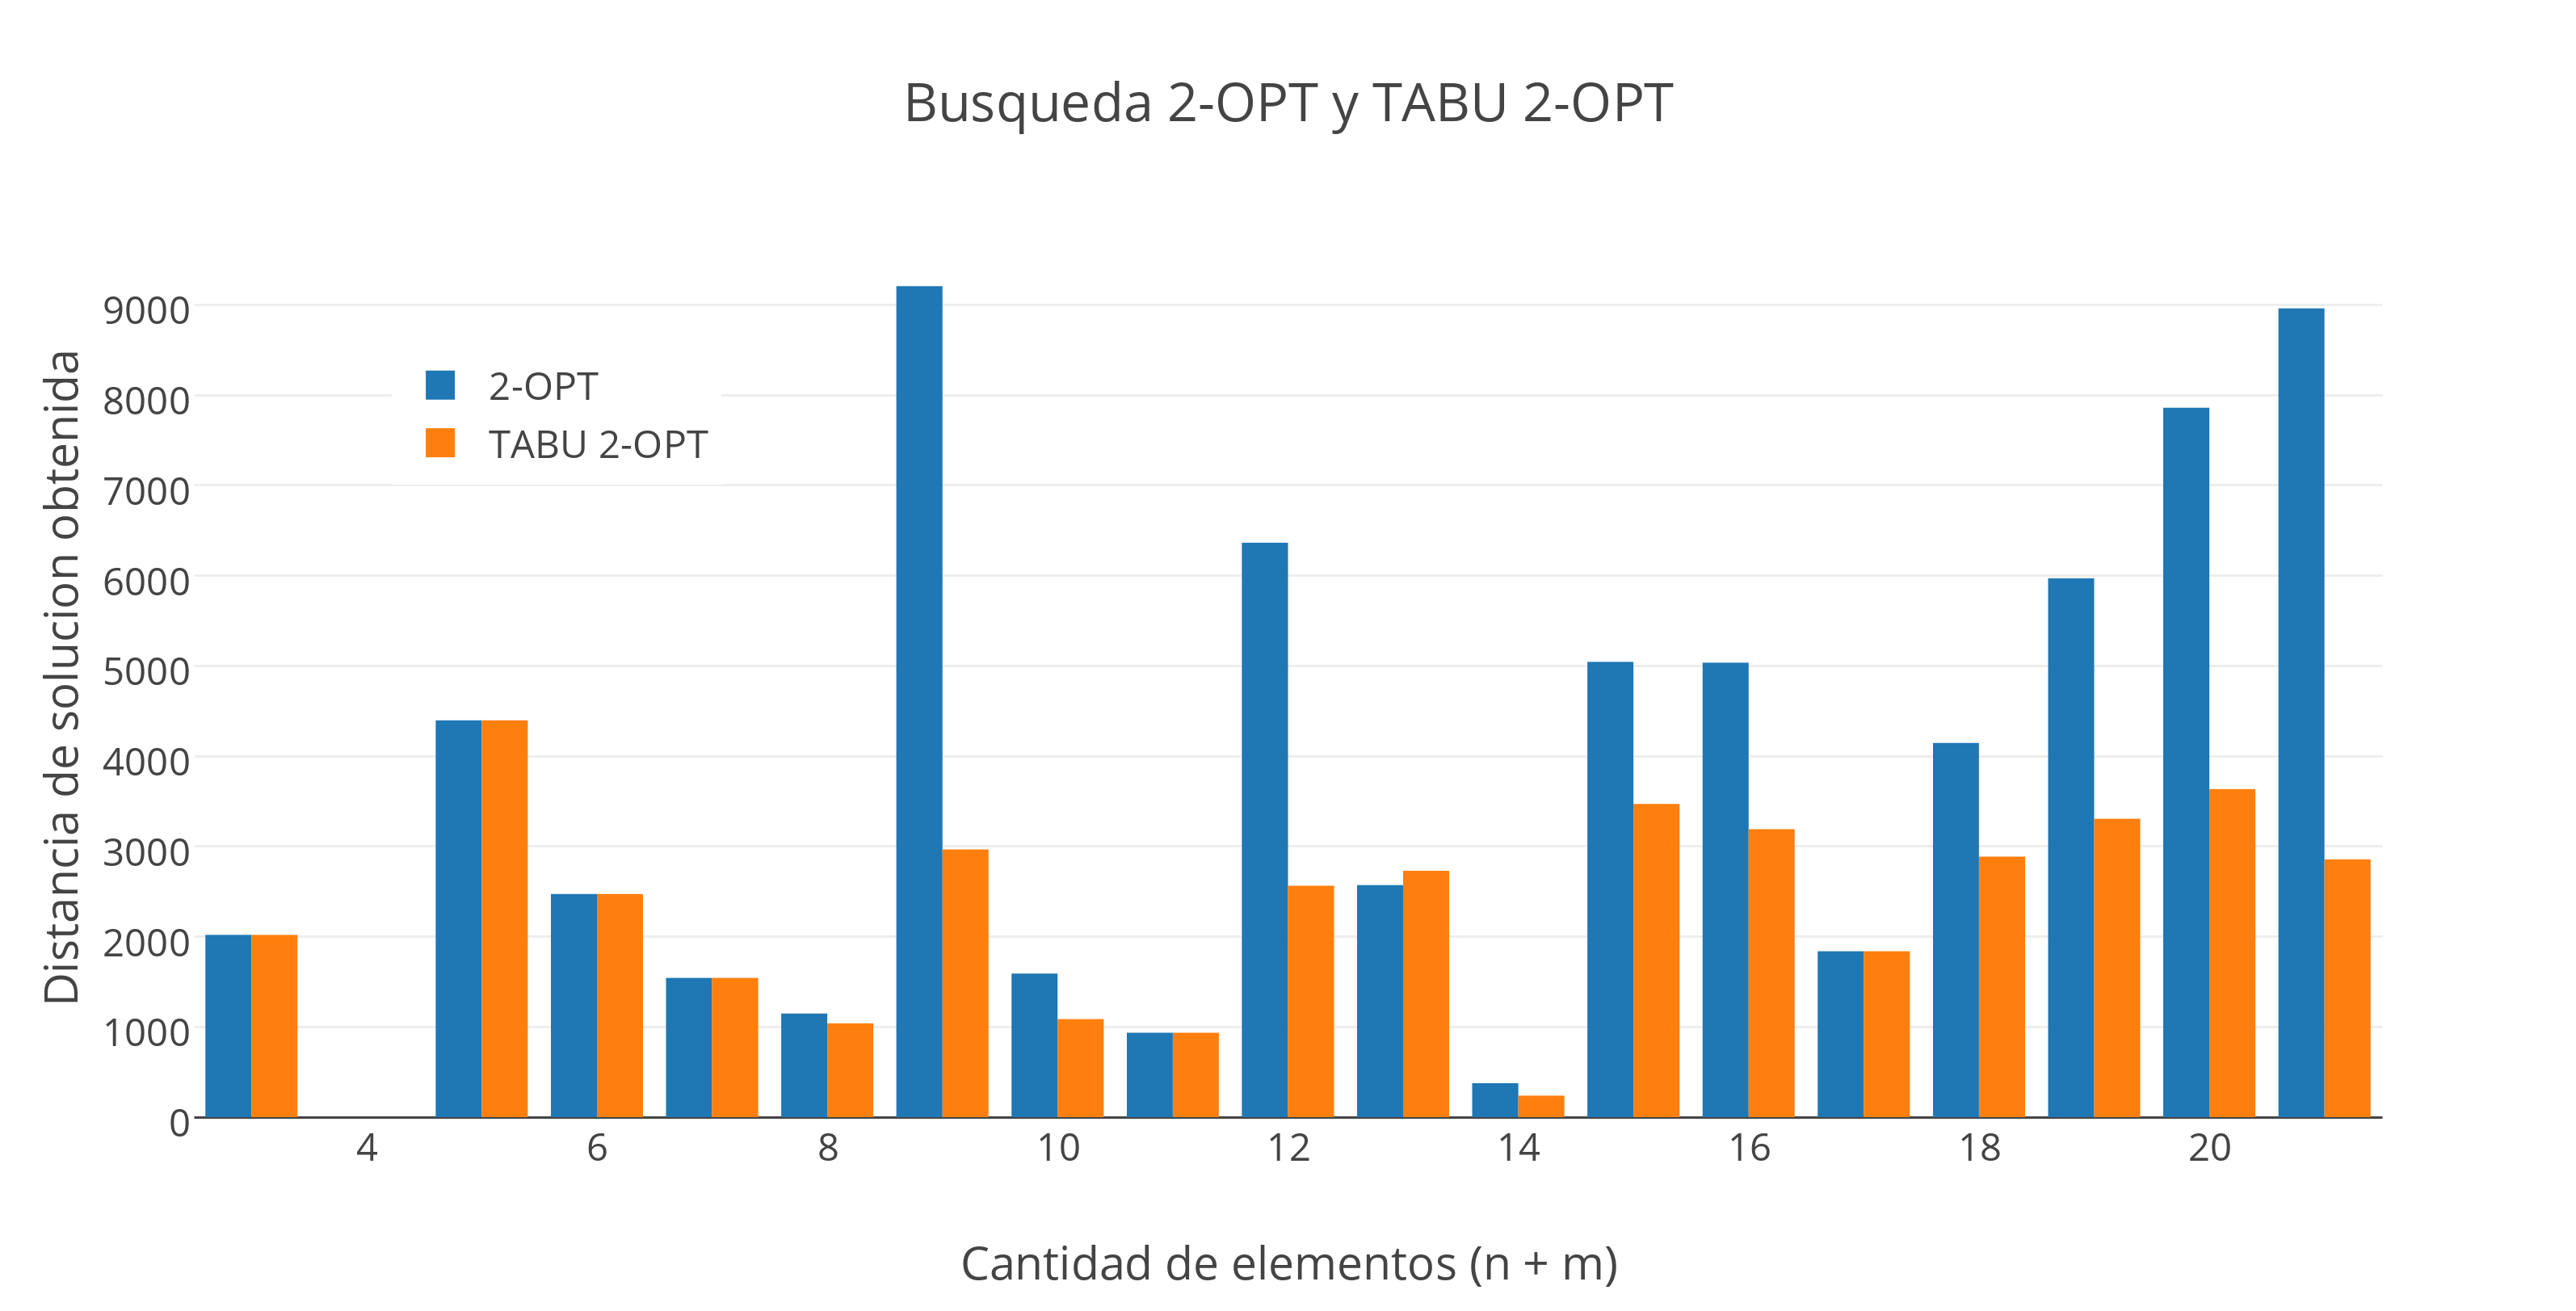
\includegraphics[scale=0.5]{./EJ4/comparativorandom2opt.png}\\
 {            \textit{Gráfico \ 4.7 - 2-OPT vs Tabu 2-OPT sobre Familia 8}}
  \end{center}
  \vspace*{0.3cm}

\vspace*{0.3cm} \vspace*{0.3cm}
  \begin{center}
 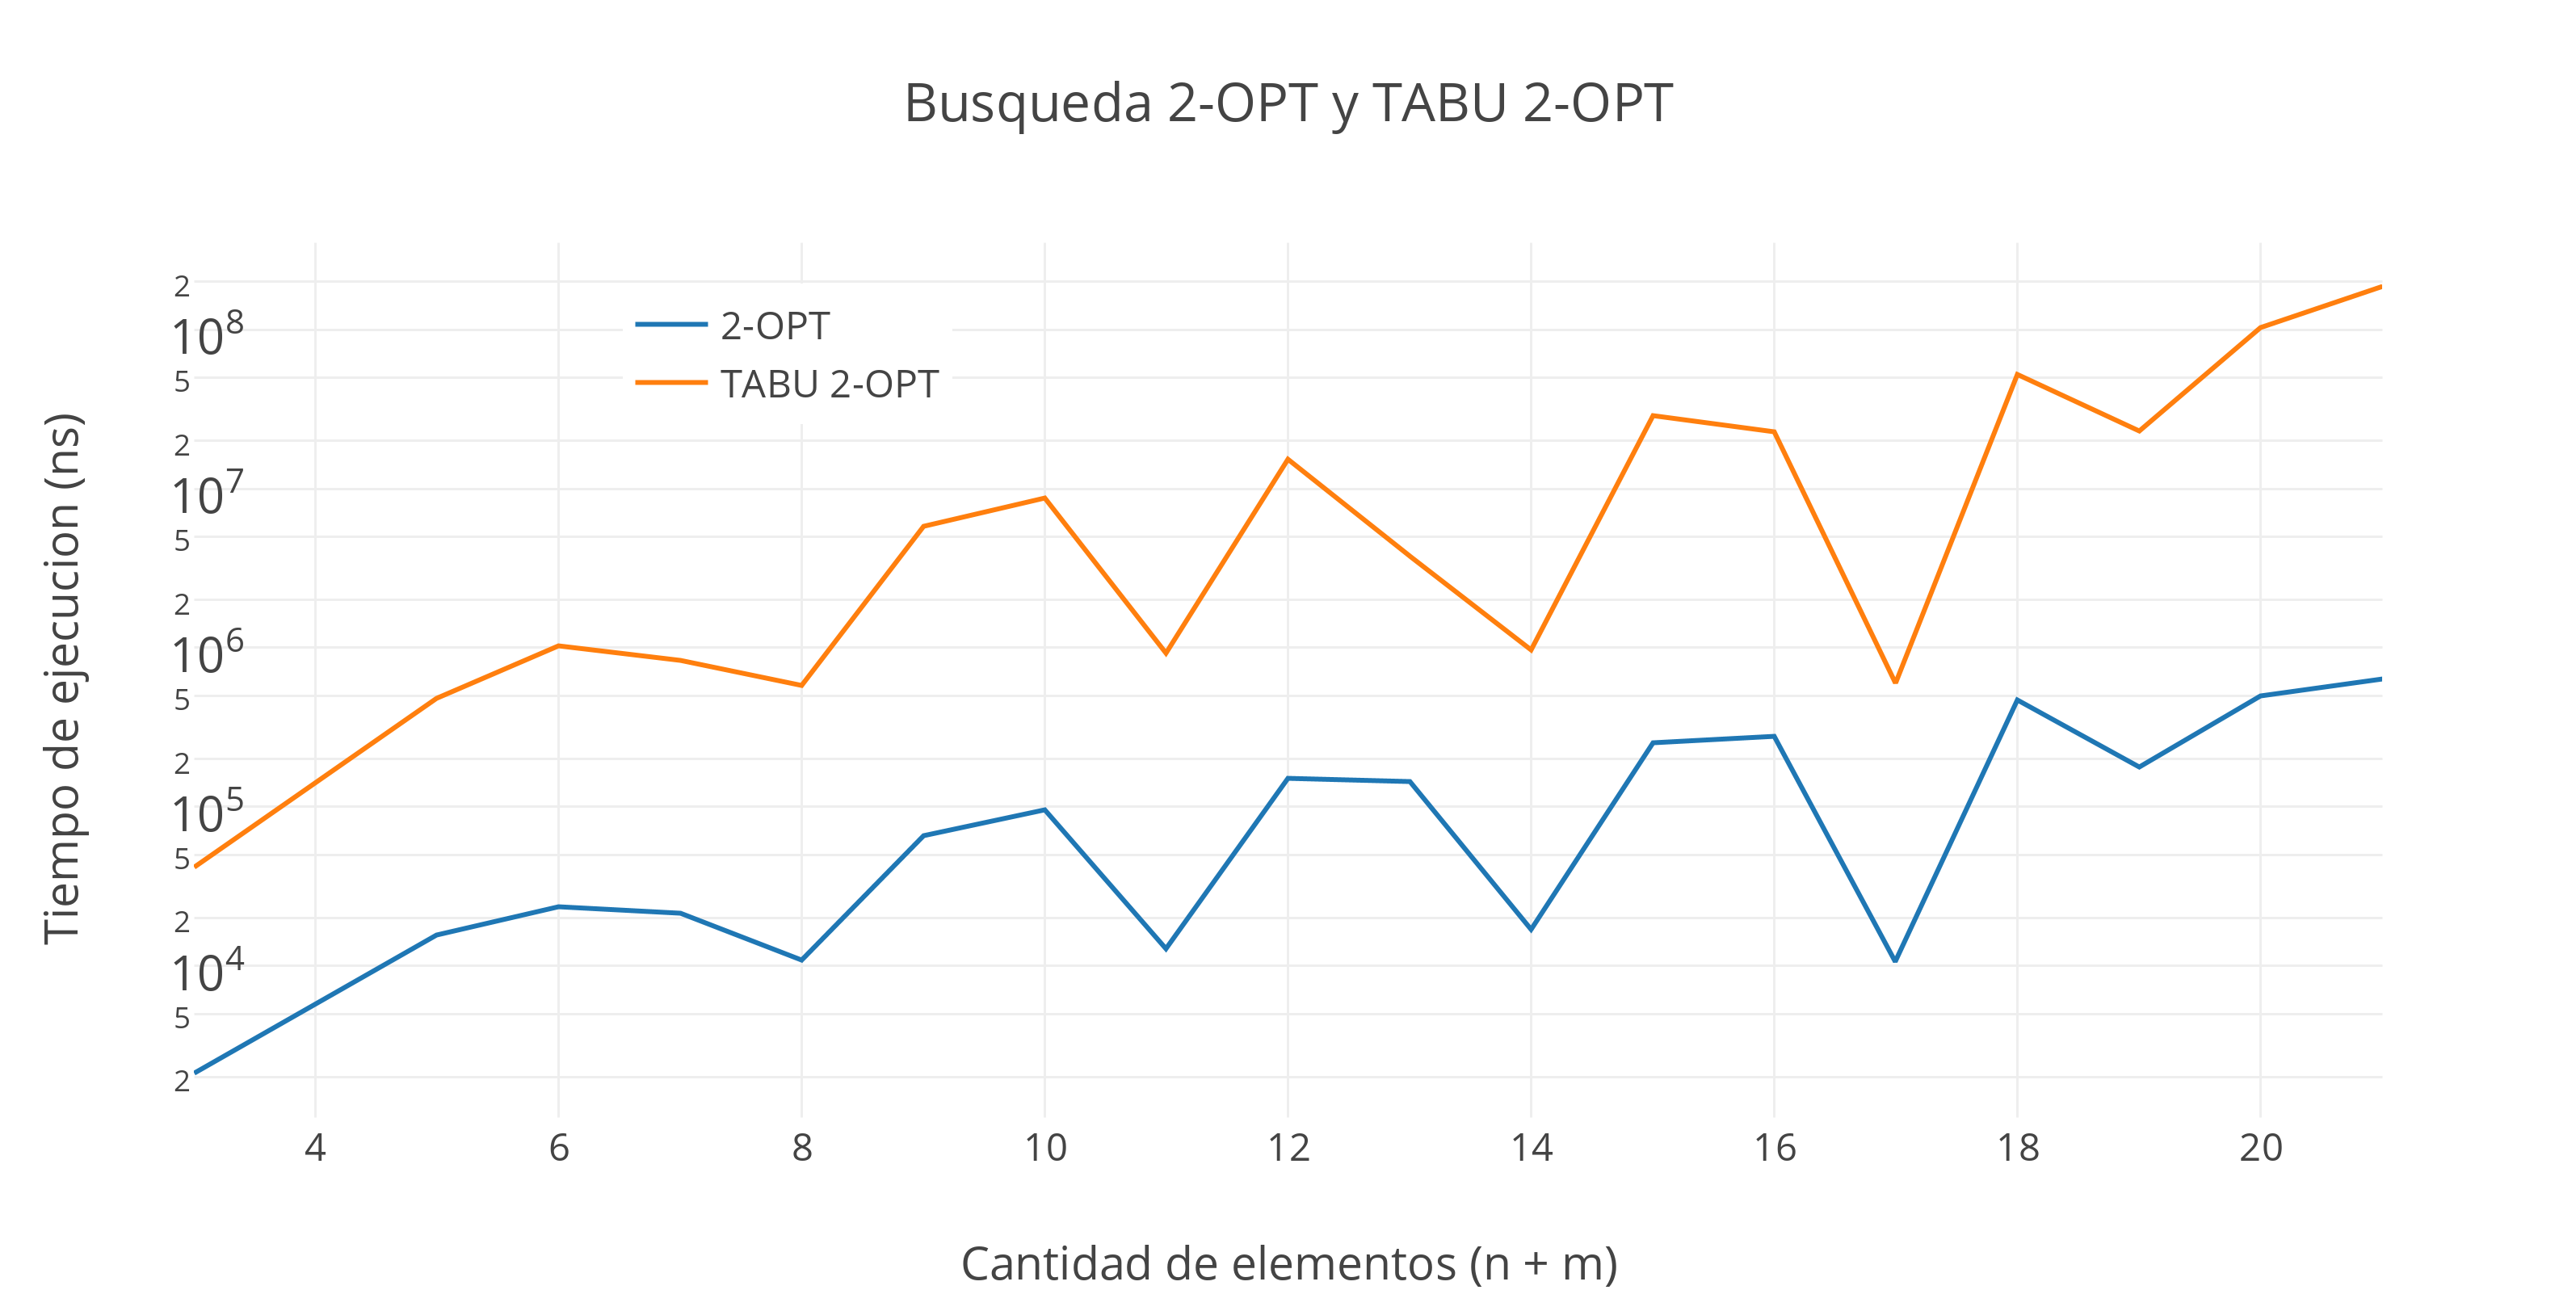
\includegraphics[scale=0.5]{./EJ4/medicionrandom2opt.png}\\
 {            \textit{Gráfico \ 4.8 - 2-OPT vs Tabu 2-OPT sobre Familia 8}}
  \end{center}
  \vspace*{0.3cm}

Luego, para 3-OPT:

\vspace*{0.3cm} \vspace*{0.3cm}
  \begin{center}
 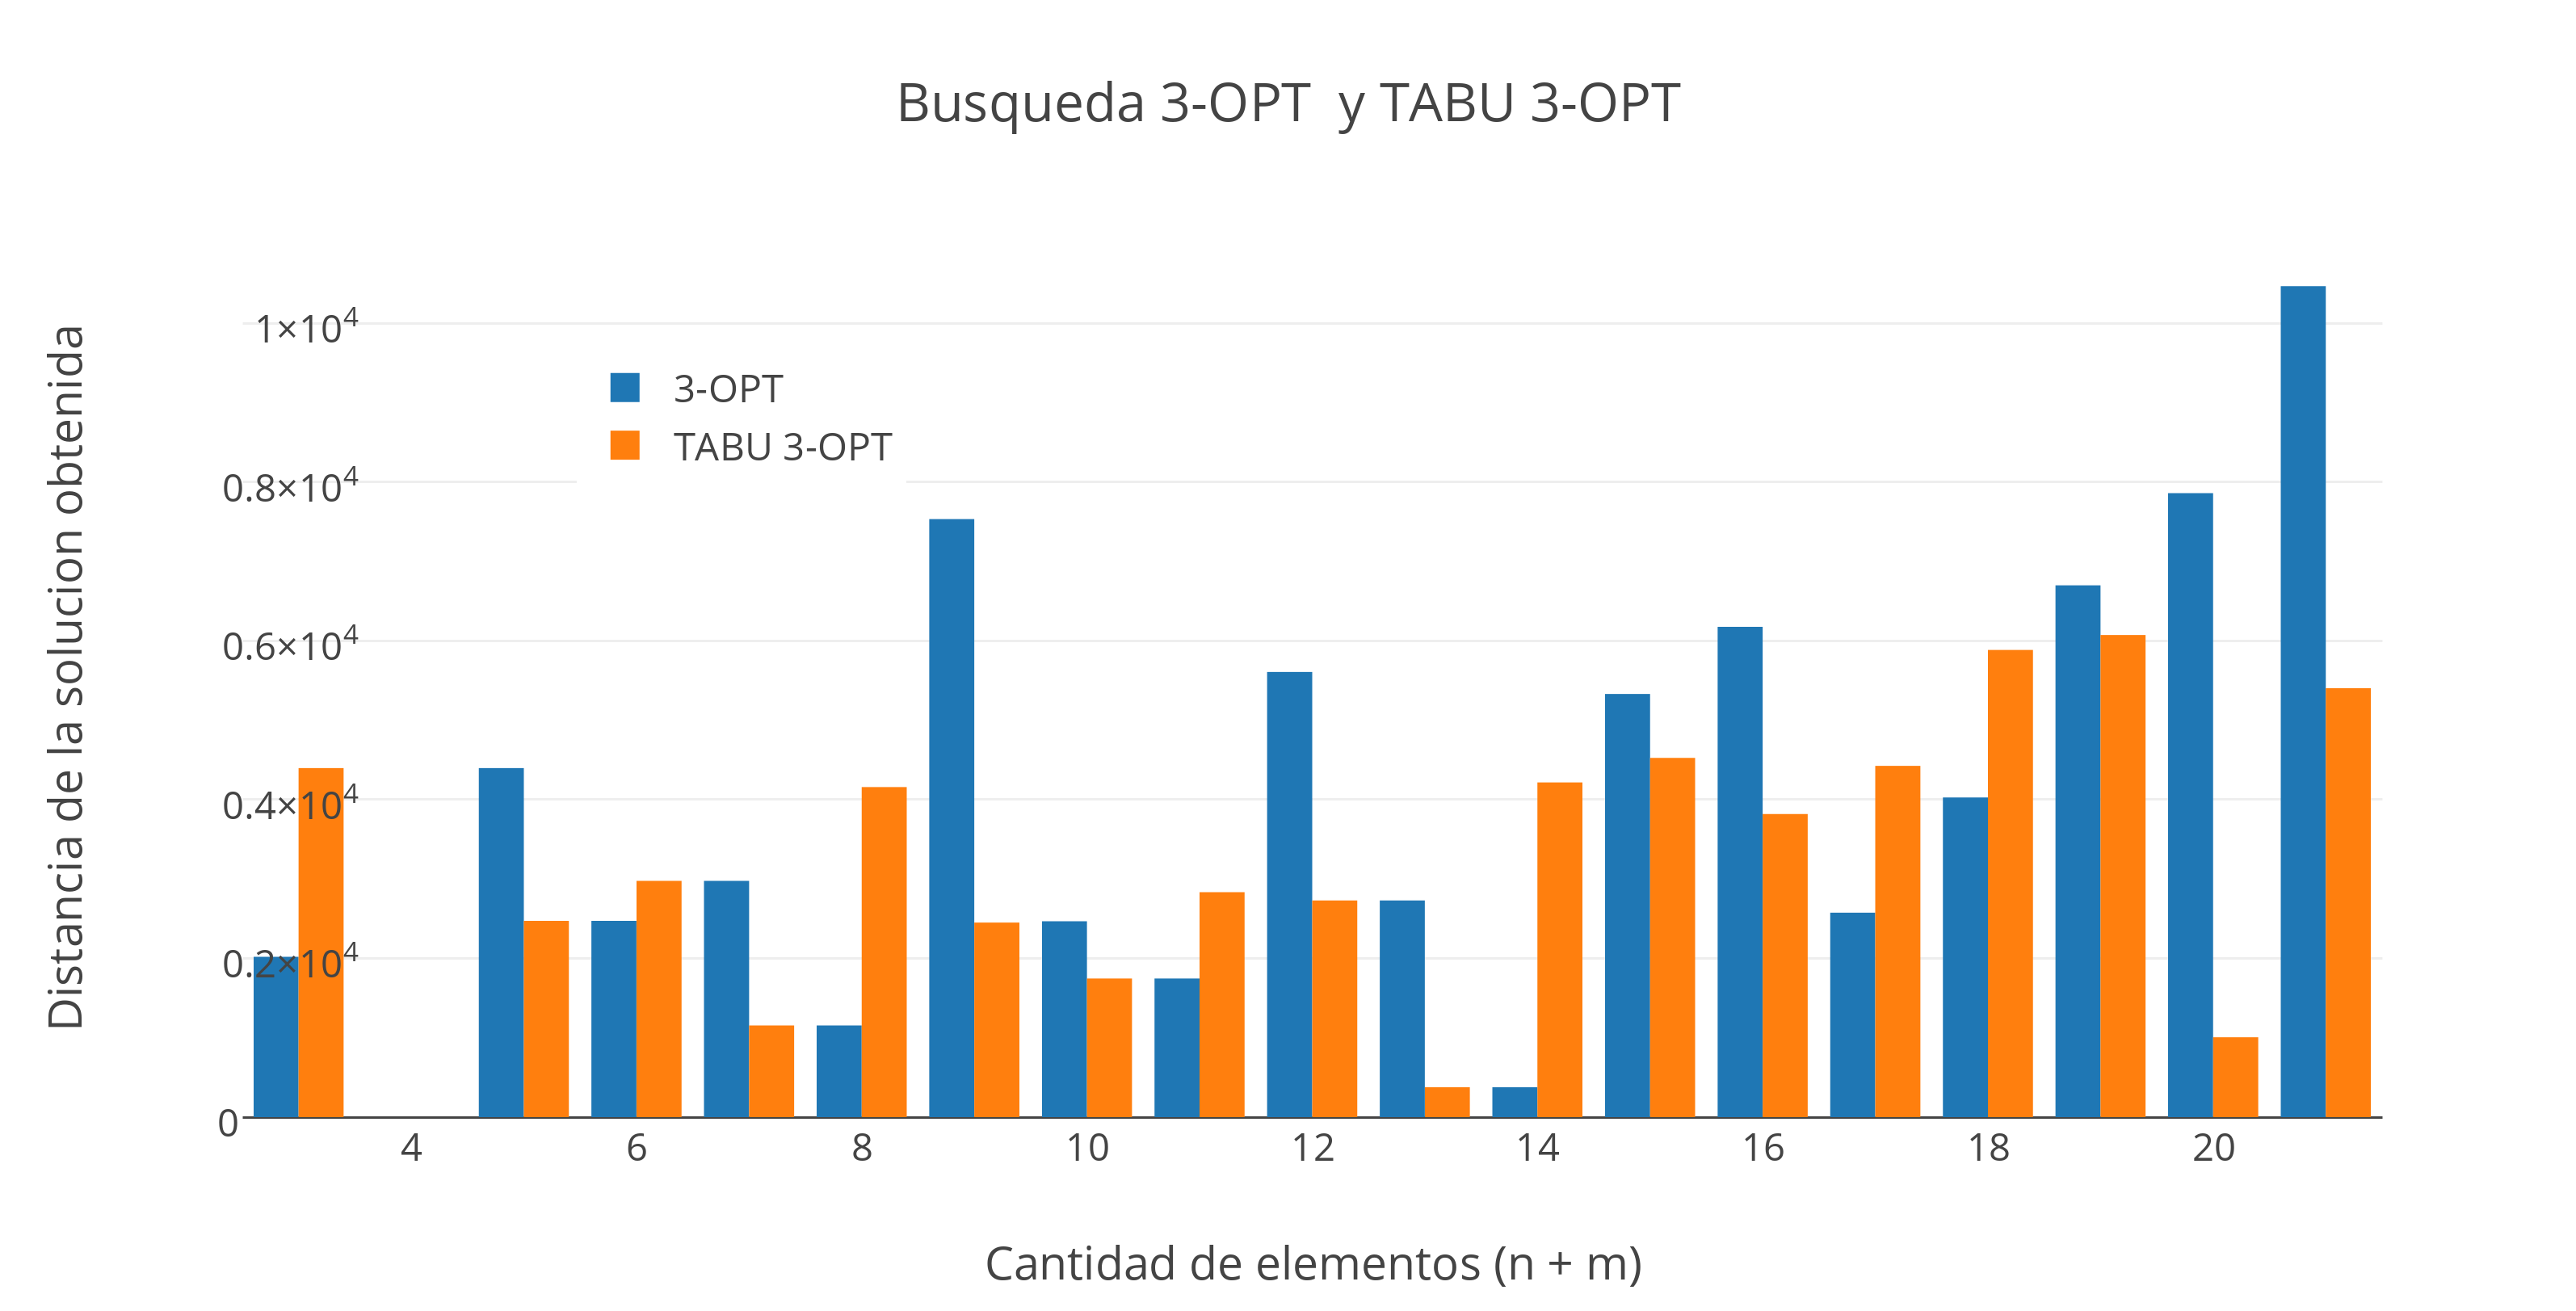
\includegraphics[scale=0.5]{./EJ4/comparativorandom3opt.png}\\
 {            \textit{Gráfico \ 4.9 - 3-OPT vs Tabu 3-OPT sobre Familia 8}}
  \end{center}
  \vspace*{0.3cm}

\vspace*{0.3cm} \vspace*{0.3cm}
  \begin{center}
 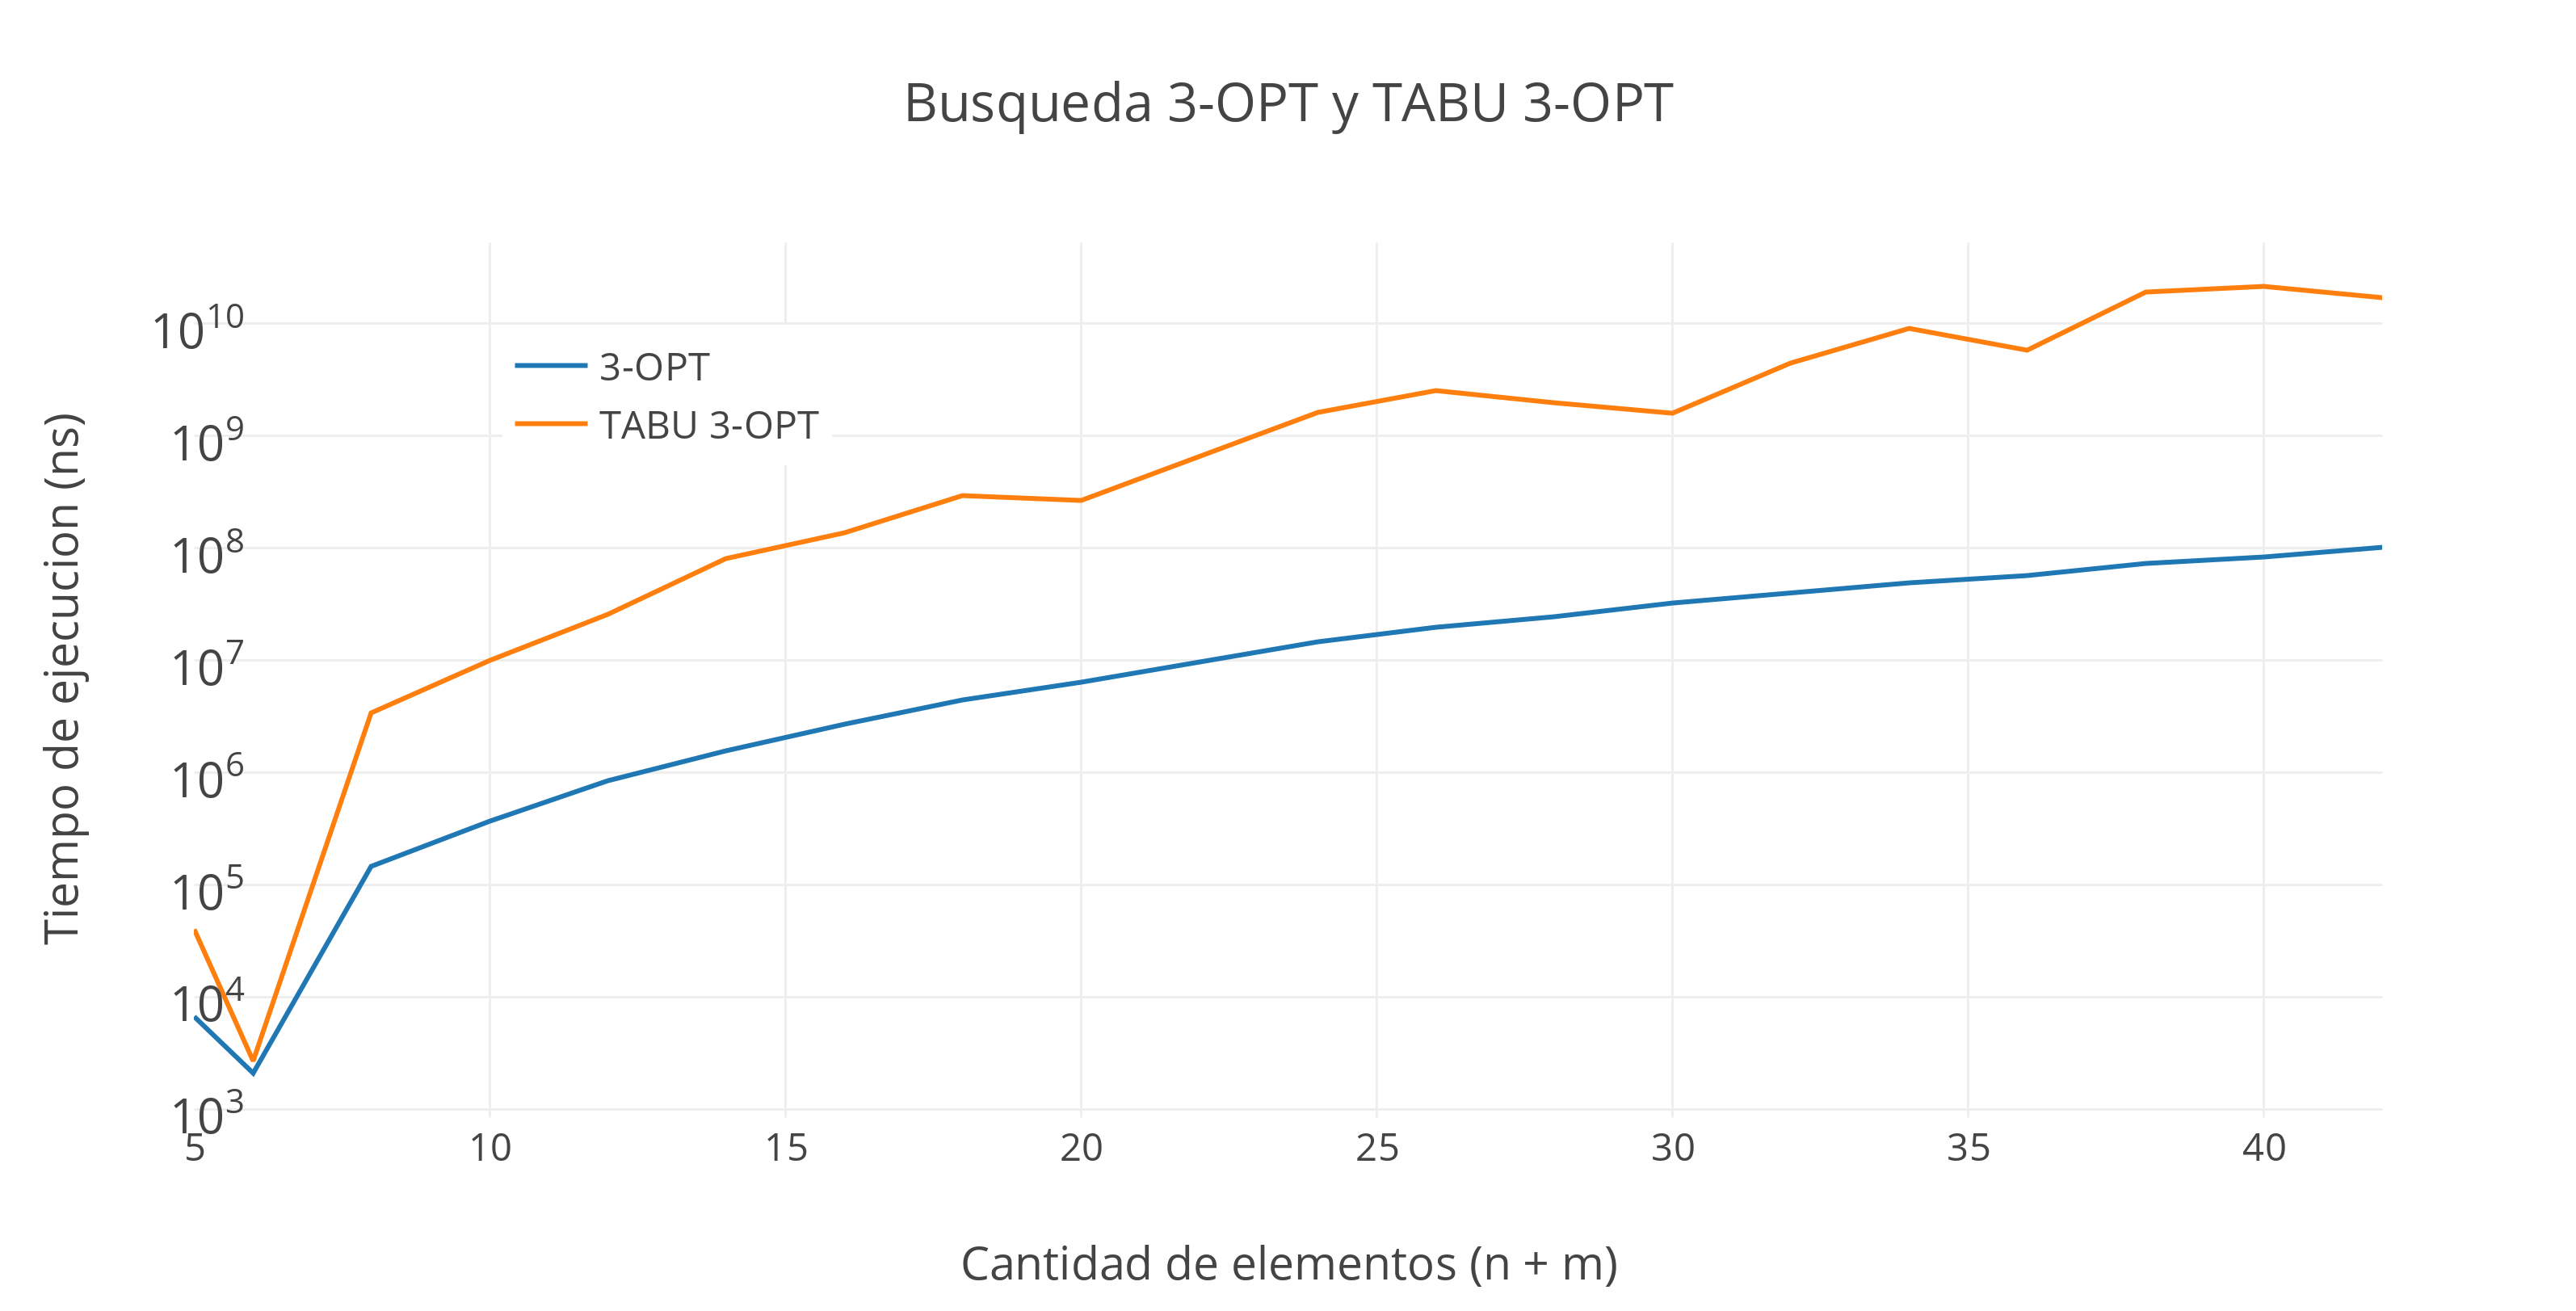
\includegraphics[scale=0.5]{./EJ4/medicionrandom3opt.png}\\
 {            \textit{Gráfico \ 4.10 - 3-OPT vs Tabu 3-OPT sobre Familia 8}}
  \end{center}
  \vspace*{0.3cm}
  
Dada la particularidad de este caso, las soluciones obtenidas y el tiempo insumido es variante tanto para las heur\'isticas como para las meta-heur\'isticas. A pesar esto tanto Tabu 2-OPT como Tabu 3-OPT obtienen soluciones mejores.
  
Comparando las soluciones de cada versi\'on de tabú search podemos observar lo siguiente: 

\vspace*{0.3cm} \vspace*{0.3cm}
  \begin{center}
 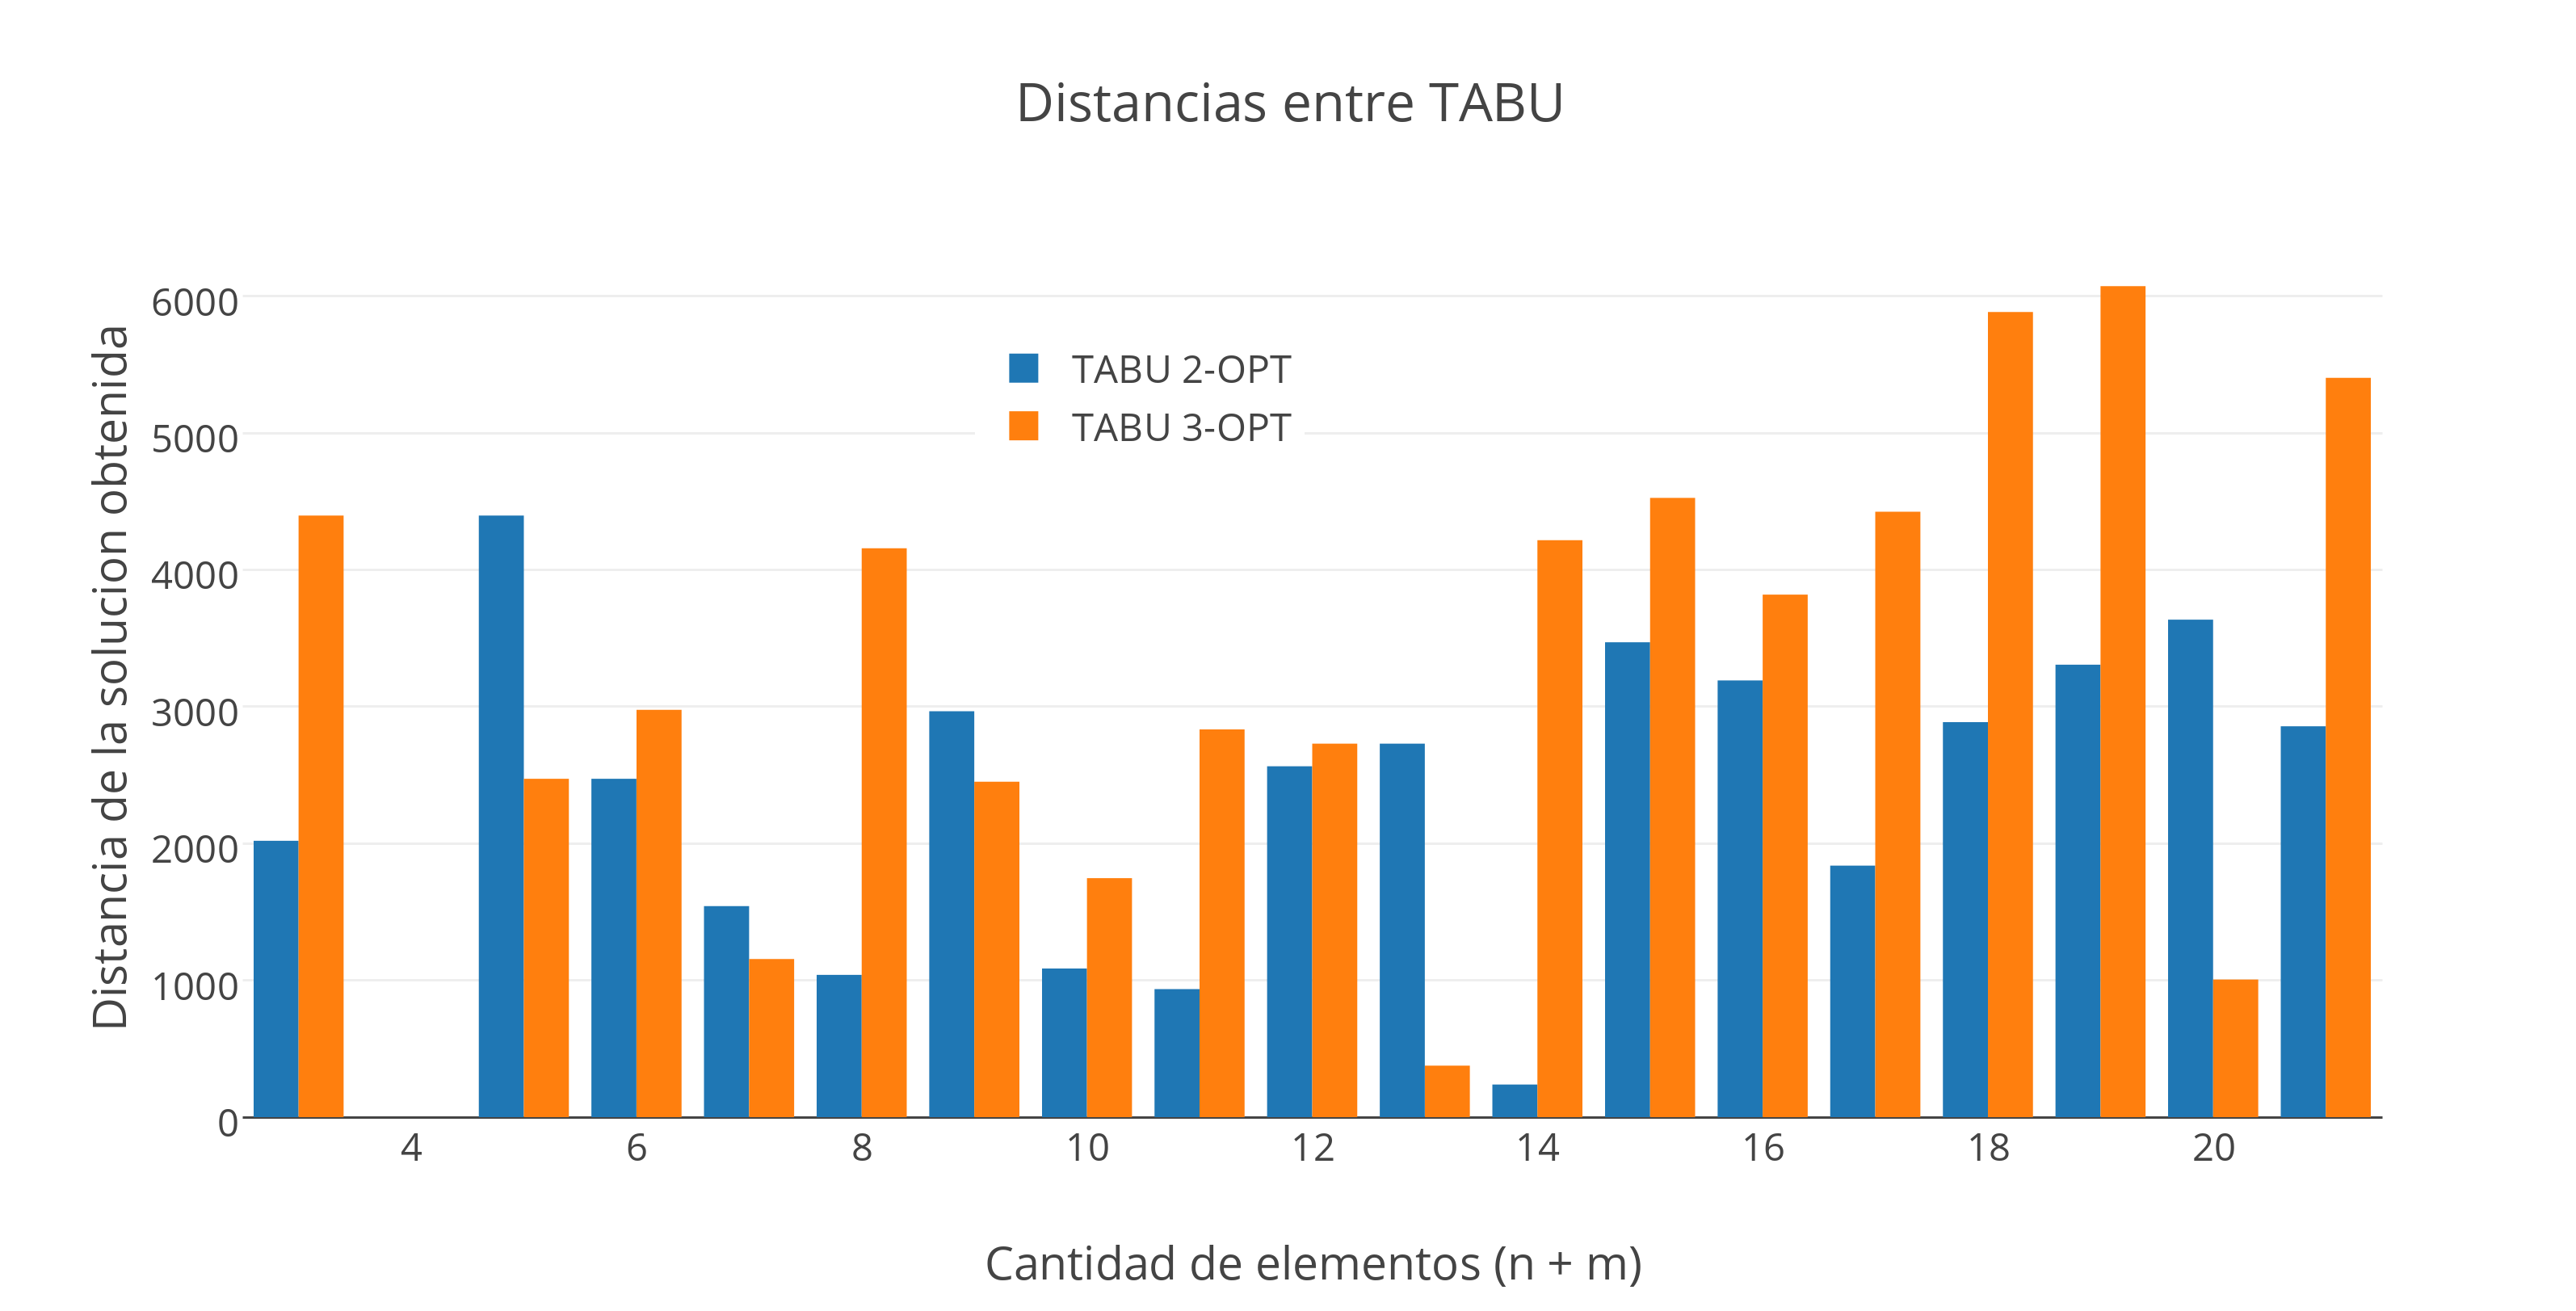
\includegraphics[scale=0.5]{./EJ4/comparativorandom.png}\\
 {            \textit{Gráfico \ 4.11 - Tabu 2-OPT vs Tabu 3-OPT sobre Familia 8}}
  \end{center}
  \vspace*{0.3cm}

\vspace*{0.3cm} \vspace*{0.3cm}
  \begin{center}
 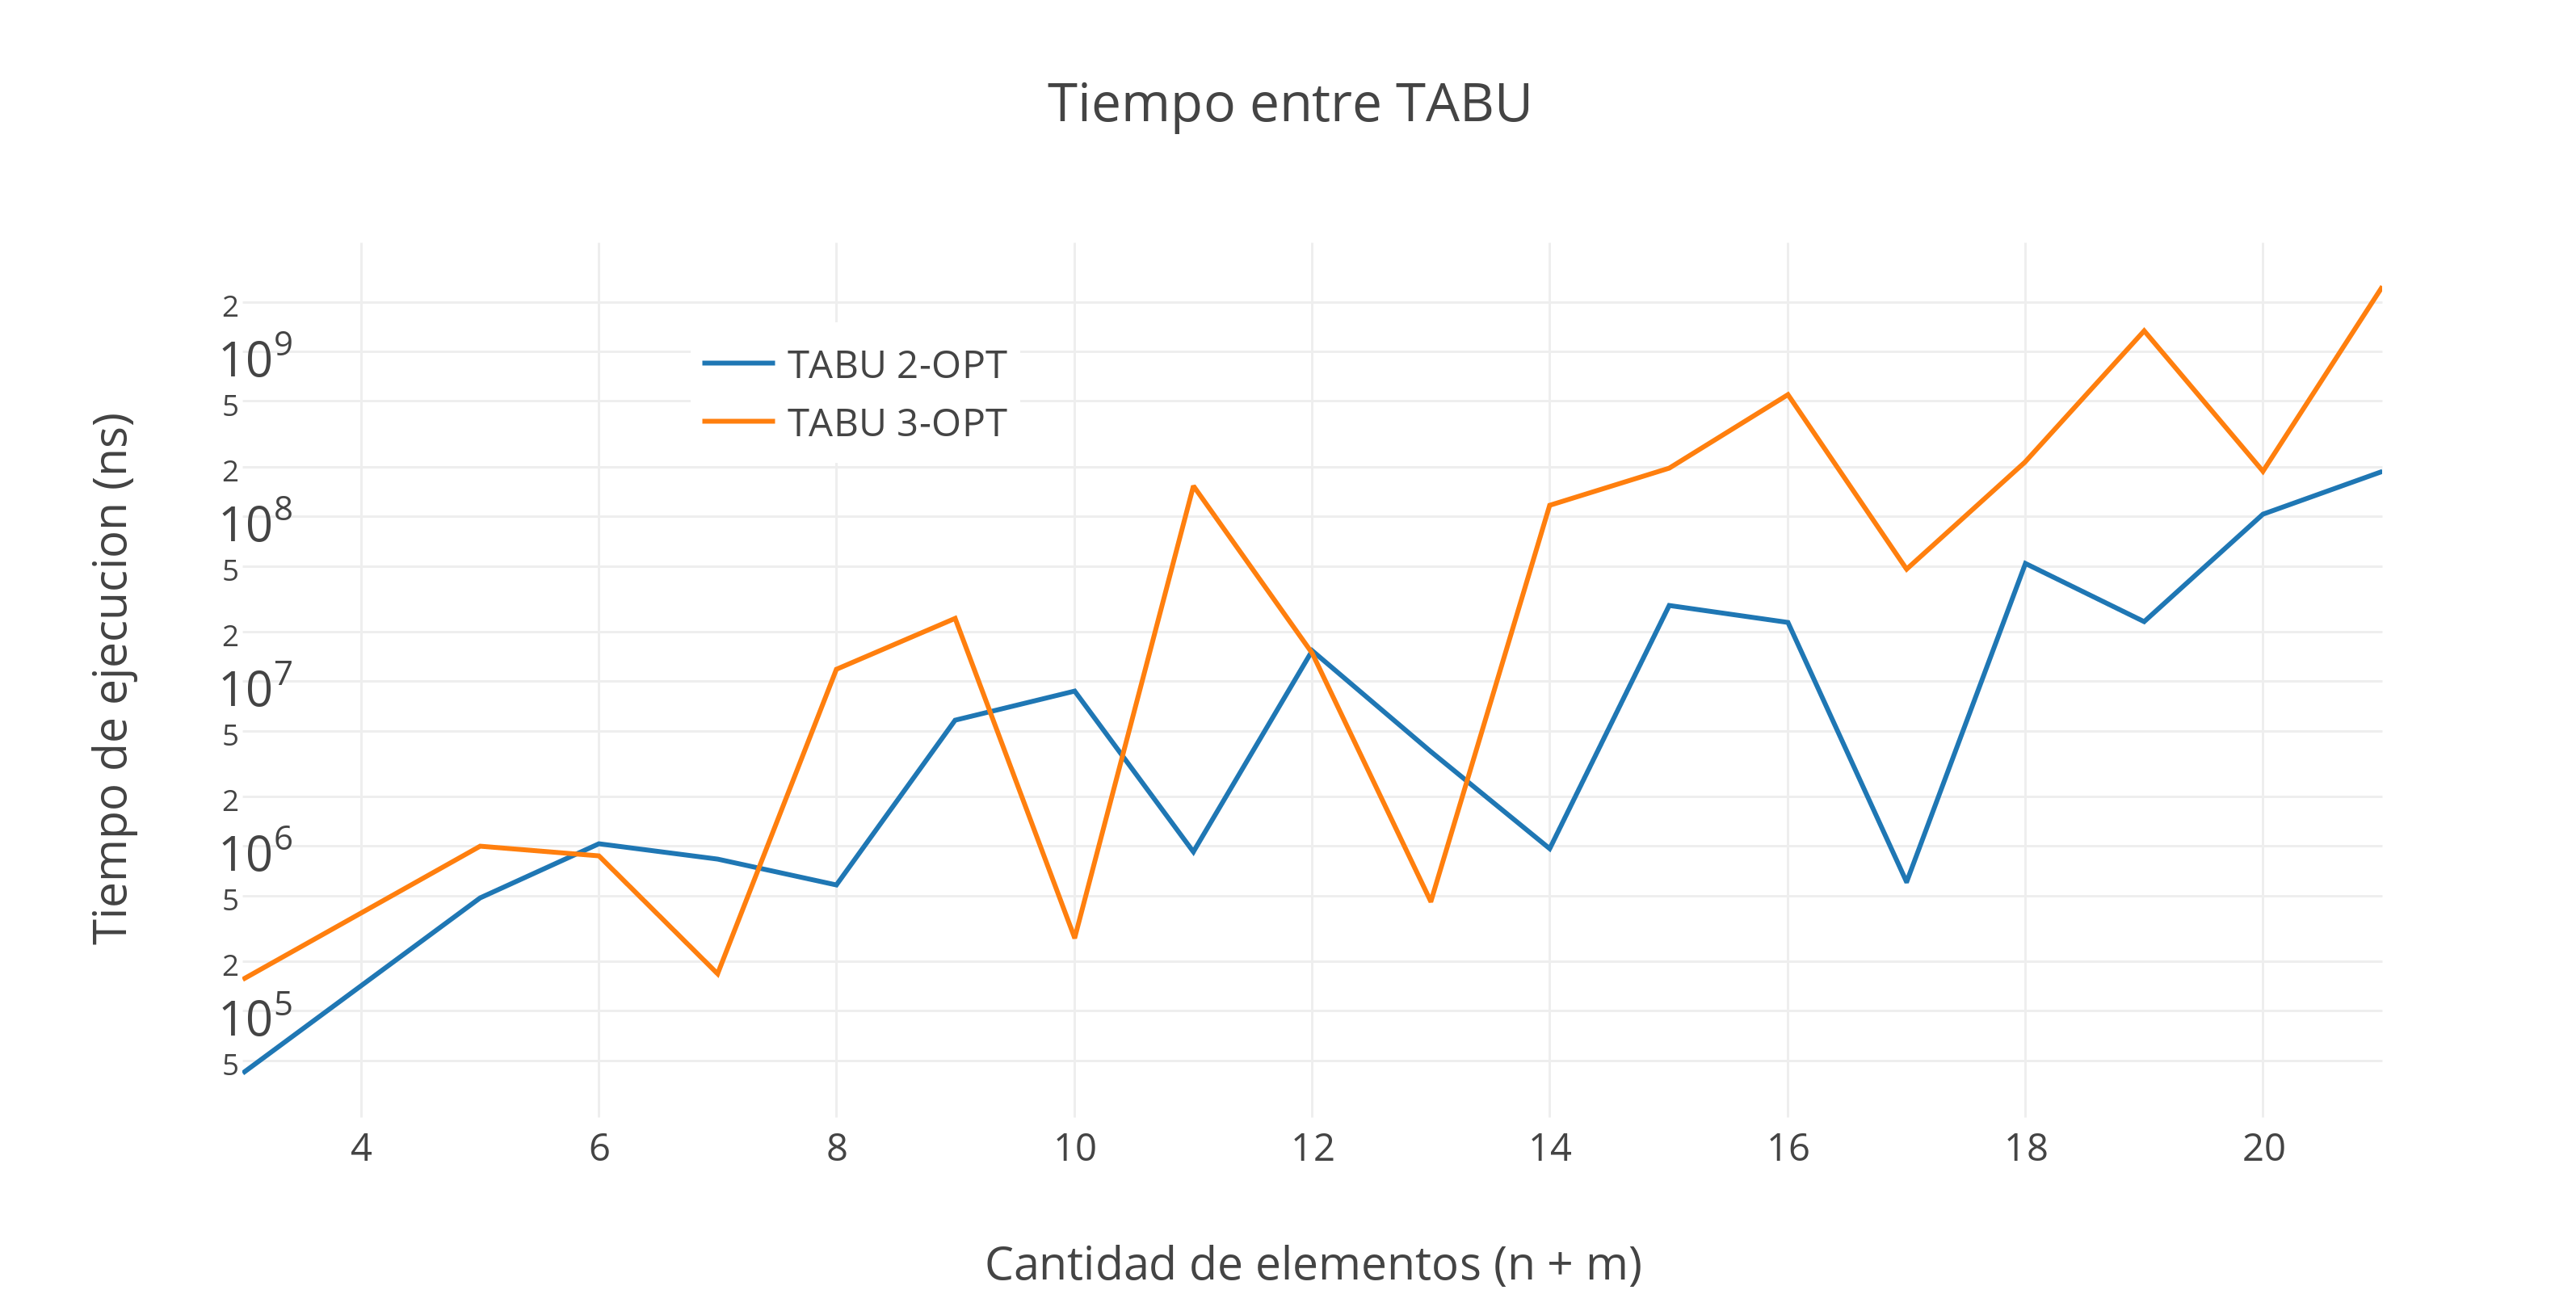
\includegraphics[scale=0.5]{./EJ4/medicionrandom.png}\\
 {            \textit{Gráfico \ 4.12 - Tabu 2-OPT vs Tabu 3-OPT sobre Familia 8}}
  \end{center}
  \vspace*{0.3cm}
  
Dando por finalizada esta familia, a pesar de la oscilacion en los resultados y mediciones Tabu 2-OPT presento un mejor desempeño que el otro. 

Como pudimos ver en este informe, para la mayoria de las familias es notoriamente mejor utilizar Tabu 2-OPT que Tabu 3-OPT ya que este ultimo insume un mayor tiempo en obtener soluciones, y dichas soluciones suelen ser siempre inferiores al primero.
Debido a la oscilacion de la familia random podra ser elegida la busqueda local 2-OPT para esta misma ya que los valores obtenidos y el tiempo que insuma llegar a estos puede ser mayor para las meta-heuristicas trabajadas.

A la hora de trabajar con estas familias y tener que elegir entre Tabu 3-OPT y la b\'usqueda respectiva, como vimos ser\'a preferible trabajar con la heur\'istica ya que esta obtendr\'a una mejor soluci\'on y en menor tiempo. Por el contrario, para el otro Tabu, obtendr\'a una solucion ampliamente mejor dejando de lado que el tiempo insumido pueda llegar a ser un poco mayor.


En adicion a lo desarrollado, podemos ver que el tiempo de ejecución del algoritmo esta ligado plenamente a la cantidad de iteraciones que realiza el algoritmo.A estas iteraciones a su vez, como también determinan a la exactitud de la solución, se las debe acotar de forma tal que se pueda obtener un trade/off beneficioso entre tiempo de computo y solucion obtenida. Para este analisis amparamos 2 opciones:
\begin{itemize}
\item Corte por cantidad de iteraciones máxima: Esta variante implica determinar un numero máximo fijo de iteraciones (por ejemplo 100), determinando un tiempo fijo de ejecución máximo.
\item Corte por criterio de calidad determinado: El criterio sería detectar cierta convergencia en la distancia minima lograda y cortar en ese limite. El criterio se basa en que si no se logra una mejora en la solución por 4 iteraciones, entonces se considera que no se puede mejorar la solucion.
\end{itemize}

La elección seleccionada fue la segunda. Esto se debe a que al analizar distintos tamaños de instancias, se podia ver que en las instancias de menor tamaño, se llegaba a una "meseta" de donde no se podia mejorar más la solucion, y las iteraciones restaantes, simplemente desperdiciaban tiempo de computo. Por otro lado, para instancias grandes, con muchos cambios posibles, se producia un corte en la mejora de la solución, ya que el algoritmo no llegaba a encontrar esa "meseta" por que cortaba las iteraciones antes de tiempo. 

Al cambiar de metodología, se logró hacer que el algoritmo se adapte al tipo de instancia, dandole el tiempo suficiente para llegar a la "meseta" de cada instancia. Cabe destacar que esta elección de corte no determinaría una solución optima, ya que cada "meseta" simboliza un minimo en la funcion de mejoras, pero no se puede asumir que ese minimo también es un ínfimo.


  \begin{center}
 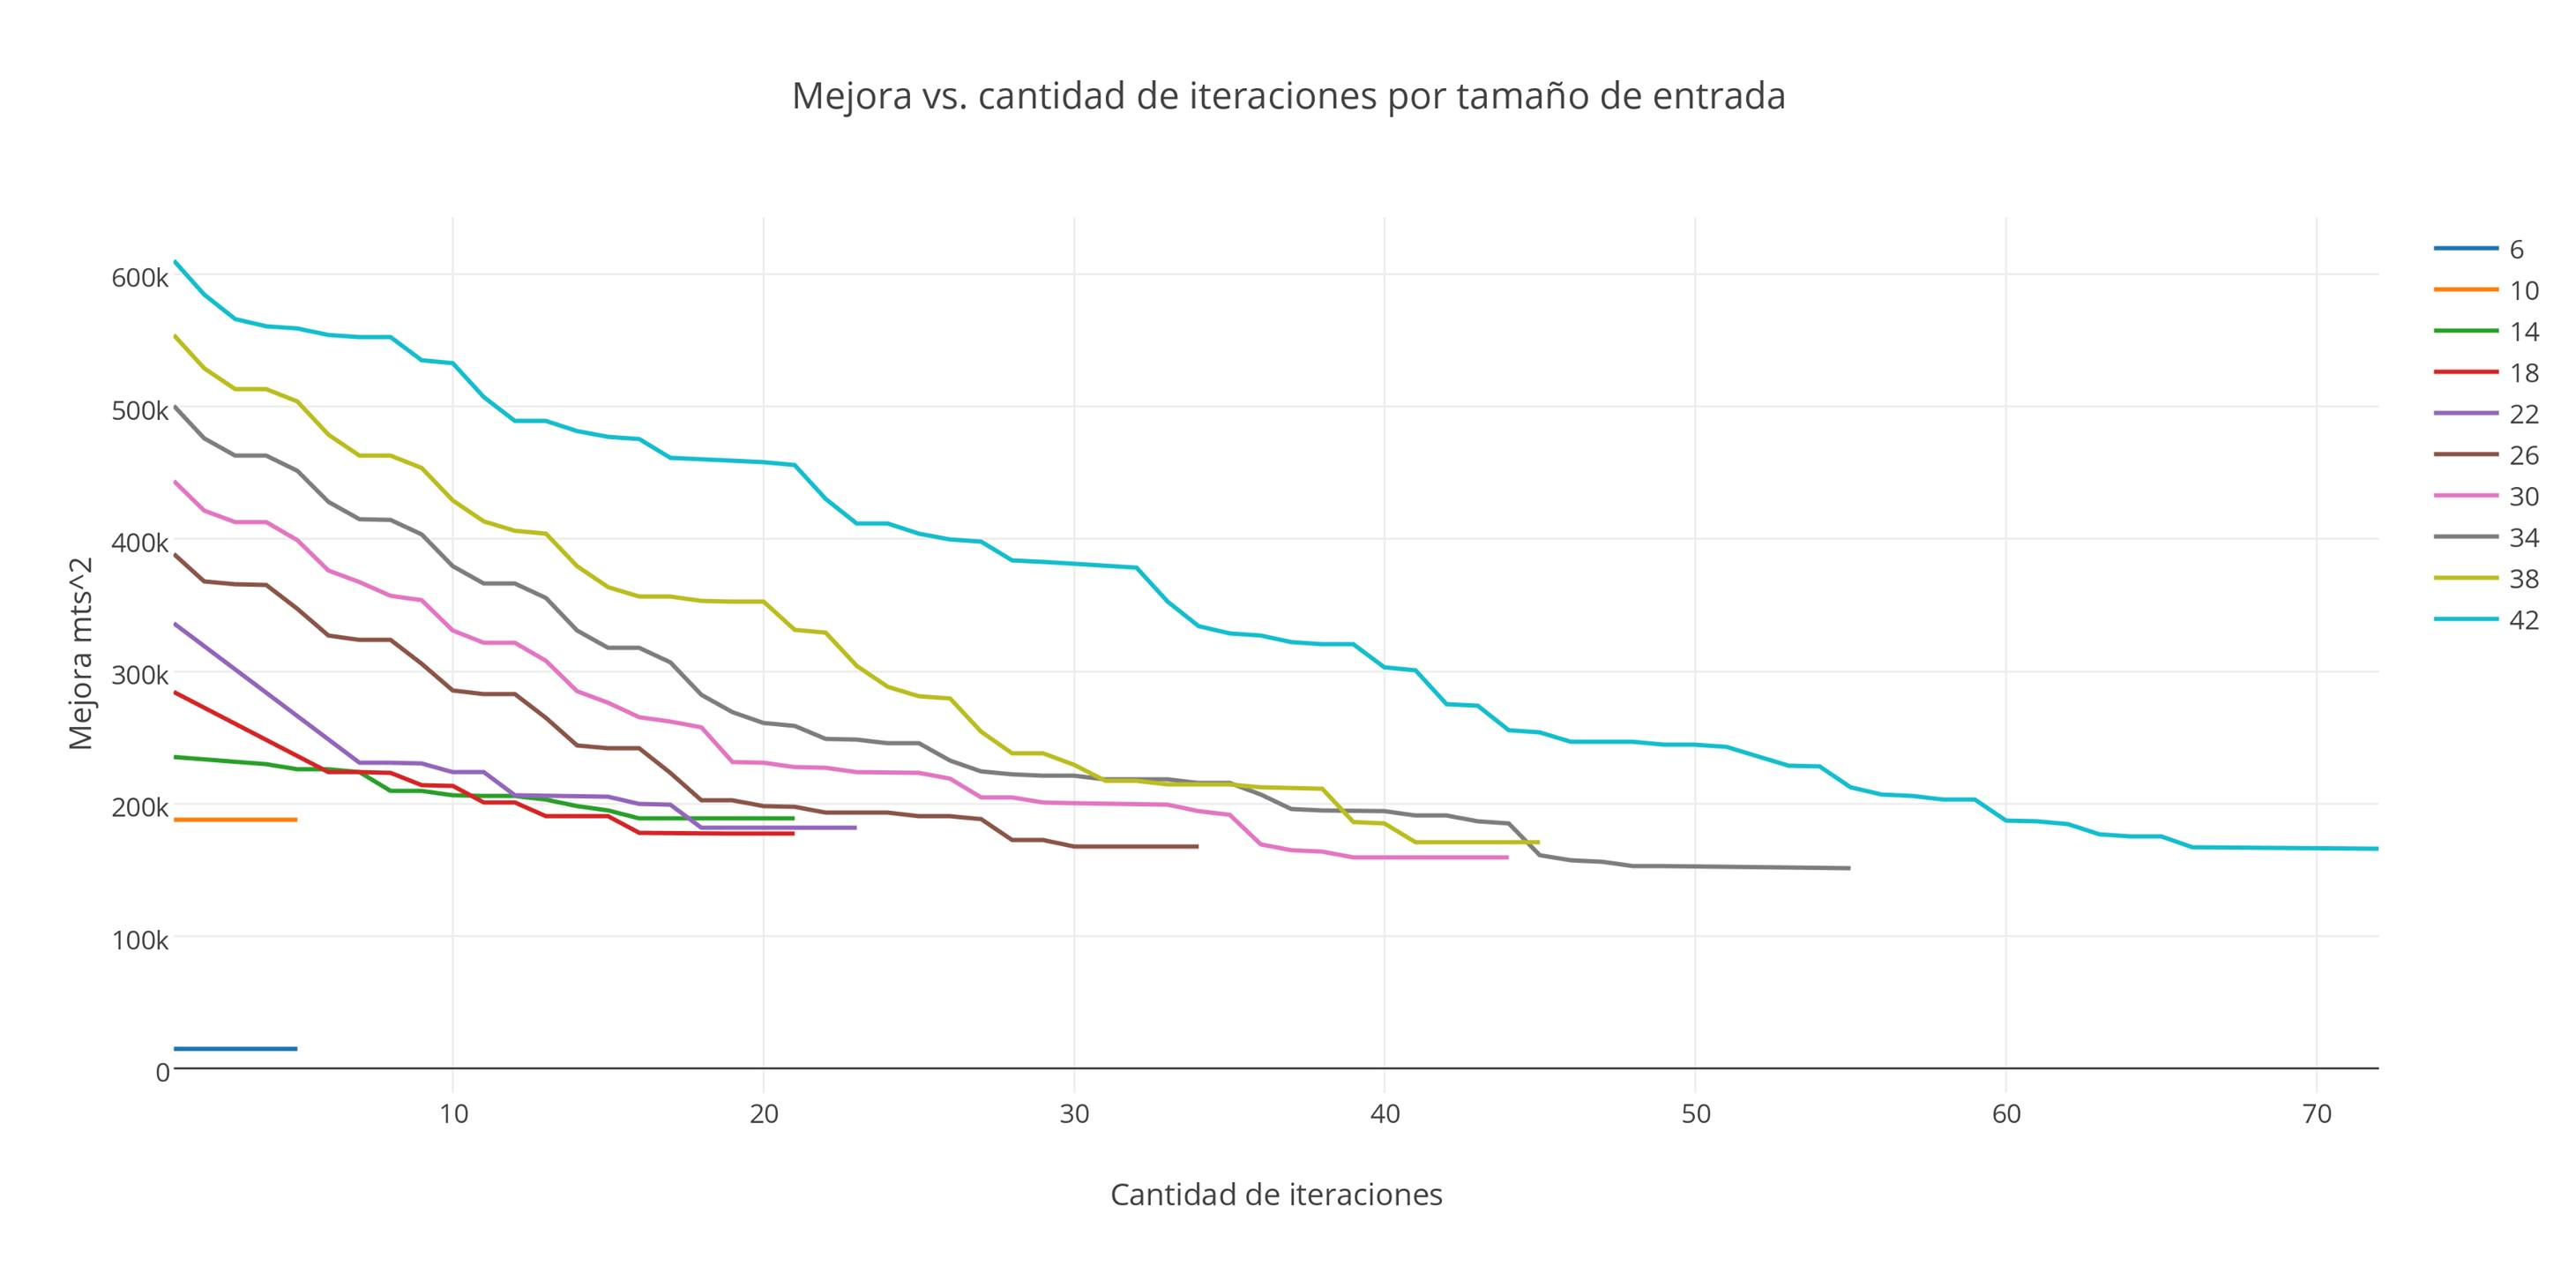
\includegraphics[scale=0.2]{./EJ4/mejora2.png}\\
 {            \textit{Instancias de distinto tamaño con cortes acordes a cada caso}}
  \end{center}
  \vspace*{0.3cm}
  

  En el gráfico se puede observar el tiempo que cada instancia de un tamaño determinado (cada linea) haya su solución a travez del algoritmo, el decrecimiento implica que la solución mejora, y cuando se detecta que ya no se pudo mejorar por un período de 4 iteraciones, entonces corta y devuelve la solución hallada como la mejor. Claramente no se puede decir que se halla la mejor solución (es decir el que produce el infimo error) pero si un minimo local para cierta vecindad de soluciones.
